%% Preamble Master Thesis
\documentclass[12pt, a4paper, twoside, openright]{report} %REPORT %chapter, section, subsection

%\linespread{1.2} % INTERLINEA

% --------- Remove Chapter from Chapter report -----

\usepackage{titlesec}
%\titleformat{\chapter}[display]
%  {\normalfont\bfseries}{}{0pt}{\Huge}

%\titleformat{\chapter}{\normalfont\Huge\bfseries}{\thechapter.}{20pt}{\huge}

\usepackage[T1]{fontenc}
\usepackage[utf8]{inputenc} % encoding used for .tex file
\usepackage[british]{babel}	% can be omitted "utf8" encoding is the default

\usepackage{amsmath}
\usepackage{amsfonts}
\usepackage{amssymb}
\usepackage{mathtools} % add tool like xrightarrow

\usepackage{multirow}
\usepackage{array}
\newcolumntype{P}[1]{>{\centering\arraybackslash}p{#1}}  % Add the centering in the tabular with fixed colum width

\usepackage{geometry} % margin and other page settings 
%\geometry{hmargin={2cm,2cm},vmargin={2cm,2cm}}
\geometry{
	left=35mm,
 	top=30mm,
 	bottom=25mm,
 	right=25mm}

\usepackage[autostyle=true]{csquotes} % to quote something!

\usepackage[labelfont=bf,textfont=md]{caption} % caption options % Figure, Table in boldface and the text normal
%\captionsetup{format=hang, font = small}
\captionsetup{font = footnotesize}
%\captionsetup{widht=0.8\textwidth}

\usepackage{graphicx} % figure object 
\usepackage{subcaption}
\graphicspath{{img}} 
%FOR DIFFERNT PATHs
% 
%\graphicspath{{path1}}
%\input{file1.tex}
%\graphicspath{{path2}}
%\input{file2.tex}
%
\usepackage{enumitem} % change the enumerate item [label=\arabic*)]

\usepackage{float} % add options for floating object: \begin{figure}[H]


%%% ----- To set header/ footer
\usepackage{fancyhdr}
%\fancyhead[LO]{\rightmark}
%\fancyhead[RE]{\leftmark }
\pagestyle{fancy}
%\fancyhf{}
\fancyhead{}
\fancyhead[RO]{\rightmark}
\fancyhead[LE]{\leftmark }
%\rhead[RO]{\rightmark}
%\lhead[LE]{\leftmark}

\usepackage{emptypage} % include NOT TRIED

\usepackage[colorlinks=true, linkcolor=blue]{hyperref} %to use autoref

\newcommand{\figRef}[1]{\mbox{Fig. \ref{#1}}}
\newcommand{\tableRef}[1]{\mbox{Table \ref{#1}}}
\newcommand{\eqRef}[1]{\mbox{Eq. \ref{#1}}}
\newcommand{\chapRef}[1]{\mbox{Chapter \ref{#1}}}
\newcommand{\secRef}[1]{\mbox{Section \ref{#1}}}



\usepackage[nottoc]{tocbibind} %Includes "References" in the table of contents

%\usepackage[backend=biber, style=numeric]{biblatex} %Imports biblatex package
\usepackage[square,numbers]{natbib}
%\addbibresource{{Introduction/biblio.bib}} %Import the bibliography file
%\addbibresource{{/home/michael/Scrivania/MasterThesis/ElaboratoFinale/capitoli/Introduction/biblio.bib}}

\title{Soft QCD parameter tuning using feed-forward neural networks}
\author{Michael Dessena}
\date{\today}

\begin{document}

\captionsetup{width=0.9\textwidth}  % set the width of all the captions

\maketitle

\abstract
-----INSERIRE ABSTRACT------


\tableofcontents
	

\graphicspath{{Introduction/}}
%INTRODUCTION
%%%%%-------PROVA-------------
\documentclass[10pt]{article}
\usepackage[british]{babel}
\usepackage{amsmath}
\usepackage{amsfonts}
\usepackage{amssymb}
\usepackage{geometry}
\geometry{hmargin={2cm,2cm},vmargin={2cm,2cm}}
\usepackage{biblatex} %Imports biblatex package
\addbibresource{{../biblio/biblio.bib}} %Import the bibliography file
%%%%%-------------------------

\begin{document}

	The \textbf{\emph{standard model of particle}} is the theory that describe all the elementary particles, the electroweak \cite{PhysRevLett.19.1264} and the strong interaction 
	
	
\printbibliography
\end{document}}
	
\graphicspath{{Hadron_Hadron_scattering/}}
% Hadron-Hadron Scatteing
%%%%%-------PROVA-------------
%\documentclass[12pt]{report}
%\usepackage[british]{babel}
%\usepackage{amsmath}
%\usepackage{amsfonts}
%\usepackage{amssymb}
%\usepackage{geometry}
%\geometry{hmargin={2cm,2cm},vmargin={2cm,2cm}}
%\usepackage{caption}
%\captionsetup{format=hang}
%\usepackage{graphicx}
%\usepackage{enumitem}
%\usepackage{float}
%
%
%
%\usepackage[colorlinks=true, linkcolor=blue]{hyperref} %to use autoref
%%%%%-------------------------

%\begin{document}


\chapter{Hadron-Hadron Scattering}
\label{chap:Hadron-HadronScattering}

In a high energy proton-proton collision we can have either soft or hard processes. Most of the time the hard processes are accompanied by soft interactions, occurring along the hadron interaction.
While the hard processes as the Higgs boson production, or the high $p_T$ jet production are well understood using perturbative QCD, the soft processes as the underlying event, the hadronization are not so well understood. In fact, these processes involving a low energy scale at which perturbative series expansion of QCD breaks down, are studied with non perturbative approaches. 

This chapter gives a theoretical introduction on some basic elements of perturbative QCD theory: the QCD factorization theorem, the fixed-order approach in perturbative QCD calculations, and finally the all-orders approaches (e.g. the parton showers).


\section{QCD factorization theorem}

The fundamental idea for the description of a hadron-hadron collision is that hadrons are made-up from partons that, at some high energy scale, can be seen as free. So the hadron-hadron interaction can be seen as an interaction between two free partons, given a sufficiently high energy scale for the interaction.
\\
This idea was developed in the framework of the deep inelastic scattering, and the Bjorken scaling observation confirms it \cite{Bjorken:1968dy}. The generalization of this concept leads to the QCD factorization theorem. 
\\   
The factorization theorem was introduced first by Drell and Yan \cite{DRELL1971578}. 
The hadron-hadron scattering cross-section is described in terms of partons extending the formalism used for deep inelastic scattering, through the following factorized formula:
\begin{equation}
\sigma_{AB}=\displaystyle\int dx_a\,dx_b\,f_{a/A}(x_a)\,f_{b/B}(x_b)\,\hat{\sigma}_{ab \rightarrow X}\quad .
\label{eq:factorization1}
\end{equation}
Where $X$ is a partonic/leptonic state and $a\,(b)$ a quark or an antiquark in the hadron $A\,(B)$. The $\sigma_{AB}$ is the hadronic cross-section while $\sigma_{ab\rightarrow X}$ is the partonic cross section that can be calculated using perturbative QCD. Finally, the $f_{a/A}\,(f_{b/B})$ is the parton distribution function in the hadron $A\,(B)$ that is dependent on $x_a\,(x_b)$ that is the momentum fraction of the total momentum of the hadron $A\,(B)$ carried by the parton. This is valid in the "scaling" limit:
\begin{equation}
	s\ \longrightarrow\ \infty\ , \qquad\qquad\qquad \frac{M_X}{\sqrt{s}}=\text{finite}\quad ;
\end{equation}
where the center-of-mass energy grows to infinity but with a fixed ratio of the X state invariant mass and the center-of-mass energy.
\\
A problem arises from the perturbative corrections from real and virtual gluon emission, in particular from the collinear gluon emissions. These contributions take to a logarithmic divergence (spoiling the convergence of the perturbative expansion). These dependencies can be absorbed by the parton distribution functions (that evolve according the DGLAP equations). This results in the scaling violation of the parton distribution functions
\begin{equation}
	f_{a/A}(x_a)\ \longrightarrow\ f_{a/A}(x_a, Q^2)\quad , 
\end{equation}  
i.e. the parton distribution function depend not only on the momentum fraction $x$, but also on the energy scale $Q^2$ of the interaction. 
\\
So, we can rewrite the factorization theorem in \eqRef{eq:factorization1} as:
\begin{equation}
	\sigma_{AB}=\displaystyle\int dx_a\,dx_b\,f_{a/A}(x_a,Q^2)\,f_{b/B}(x_b,Q^2)\,\hat{\sigma}_{ab \rightarrow X}\quad .
\label{eq:factorization2}
\end{equation}
At this point the \emph{finite} corrections to the leading-logarithmic cross section in the perturbative expansion are specific for each process (i.e. they are not universal, but they are process dependent). This leads in the \eqRef{eq:factorization2} to the following series in $\alpha_s$ (the coupling constant of QCD theory):
\begin{equation}
	\sigma_{AB}=\displaystyle\int dx_a\,dx_b\,f_{a/A}(x_a,\mu_F^2)\,f_{b/B}(x_b,\mu_F^2)\,\left[\hat{\sigma}_0+\alpha_s(\mu_R^2)\hat{\sigma}_1+\dots\right]\quad .
\label{eq:factorization3}
\end{equation}
In \eqRef{eq:factorization3} two scales enter the formula:
\begin{itemize}
	\item[--] The \textit{factorization scale} $\mu_F$: this scale is related to the resolution with which the hadron is being probed, separates long- and short- distance physics processes.
	\item[--] The \textit{renormalization scale} $\mu_R$: the scale at which is evaluated the strong coupling constant $\alpha_s$. The dependence of $\alpha_s$ on the renormalization scale is related to different effects such as  the vacuum polarization, the quark self-energy, the vertex corrections, and the gluon loop corrections to the elementary three-gluon and four-gluon couplings.
\end{itemize}

The higher-order corrections to the cross section in \eqRef{eq:factorization3} are important because they lead to an higher accuracy in the cross section prediction, gradually reducing the dependencies on $\mu_R$ and $\mu_F$. In absence of an all-order prediction, a choice for the two scales have to be taken.
Typically, the scales are assumed to be equal: in the Drell-Yan process the standard choice is $\mu_F=\mu_R=M$, with $M$ the lepton-pair mass \cite{Campbell2006}; other cases are the invariant masses of $Z$-boson, top quark or jet transverse energy to study \cite{Campbell2006} the production cross sections for Z-bosons, top quarks and large $E_T$ jets respectively.

The parton distribution functions used to describe a hard scattering are solution to the DGLAP (Dokshitzer–Gribov–Lipatov–Altarelli–Parisi) equations \cite{Lipatov:400357, Gribov:427157, ALTARELLI1977298, Dokshitzer:1977sg}
\\
\begin{equation}
	\mu_F^2\frac{\partial f_{i/H}(x,\mu_F^2)}{\partial\mu_F^2}=\displaystyle\sum_j\frac{\alpha_s(\mu_F^2)}{2\pi}\displaystyle\int_x^1 \frac{dz}{z}\, P_{i\,\rightarrow\,j}(z)\ f_{j/p}\left(\frac{x}{z},\mu_F^2\right)\quad ,
\end{equation}
\\
where $P_{i\,\rightarrow\,j}$ are the so-called splitting functions: they are the probability that a parton of type $i$ emits a parton $j$ (a quark or a gluon) carrying a fraction $z$ of the $i$-parton momentum.
\\
The splitting functions have the following perturbative expansions in $alpha_s$: 
\begin{equation}
	P_{i\,\rightarrow\,j}(x,\alpha_s)=P_{i\,\rightarrow\,j}^{(0)}(x)+\frac{\alpha_s}{2\pi}P_{i\,\rightarrow\,j}^{(1)}(x)+\dots\quad .
\end{equation}
\\
This procedure has been used to calculate cross-sections for many Standard Model processes in $p\overline{p}$ and $pp$ scattering respectively at Tevatron and LHC energies as shown in \figRef{figure:StandardModelCrossSections}.

\begin{figure}[!htb]
	\centering 
	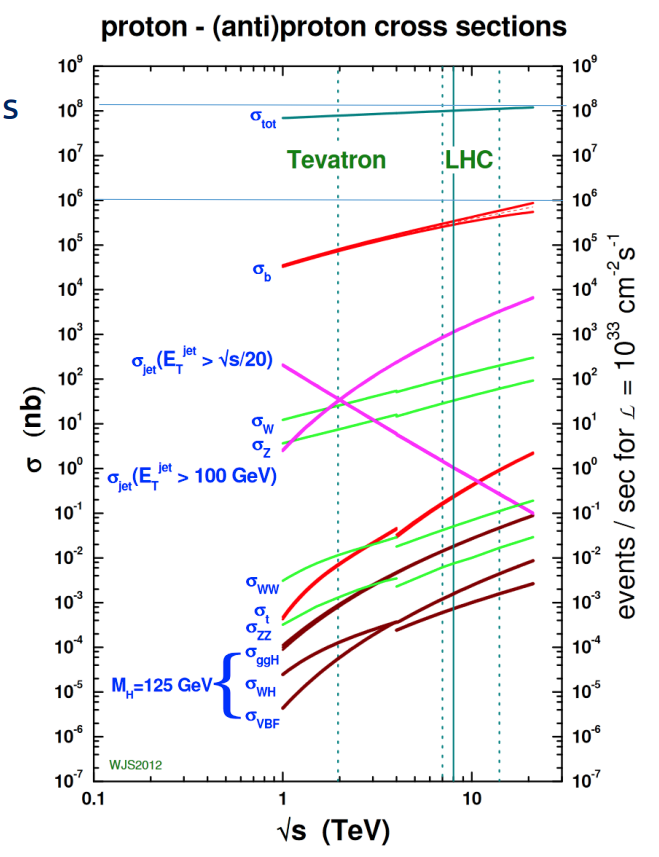
\includegraphics[width=12cm]{img/StandardModelCrossSections_color.png}
	\caption{Next-to-leading order cross sections at Tevatron and LHC colliders energies (the splitting are at the transition between $p\overline{p}$ and $pp$ cross section). Figure from \cite{StirlingPrivate}}
	\label{figure:StandardModelCrossSections}
\end{figure}

The parton distribution functions dependence on $Q^2$ can be derived theoretically via the DGLAP equations. Instead, the $x$ dependence is obtained fitting the deep-inelastic and other hard-scattering processes experimental data.
The experimental coverage in $(x,Q^2)$-plane is shown in \figRef{figure:xQ2planeCoverage} 
where is also underlined the relationship between $(x,Q^2)$ and kinematic variables in Drell-Yan processes for a final state with invariant mass $M$ and rapidity $y$ (further details in section 2 of \cite{Campbell2006}). Assuming that the factorization scale $Q$ is equal to $M$ (The reference center of mass energy is $13\ \mathrm{TeV}$), for two incoming partons with four-momentum respectively $p_1$ and $p_2$, the relations of their x (labeled as $x_1$ and $x_2$) with $s$, $y$ and $M$ are:  
\begin{equation}
	\begin{aligned}
		&p_1^\mu=\frac{\sqrt{s}}{2}(x_1,0,0,x_1)\\
&p_2^\mu=\frac{\sqrt{s}}{2}(x_2,0,0,-x_2)
	\end{aligned} \quad\Longrightarrow\quad x_1=\frac{M}{\sqrt{s}}e^y\qquad x_2=\frac{M}{\sqrt{s}}e^{-y} \quad ,
\end{equation}
where  $s=(p_1^\mu+p_2^\mu)^2$. For example the figure shows that the production of a final state with invariant mass $M=100\ \mathrm{GeV}$ and rapidity $y=2$ is given by the interaction of two hadrons with $x_1\approx0.05$  and $x_2\approx0.001$ with $Q^2=10^4\ \mathrm{GeV^2}$


\begin{figure}[!htb]
	\centering 	
	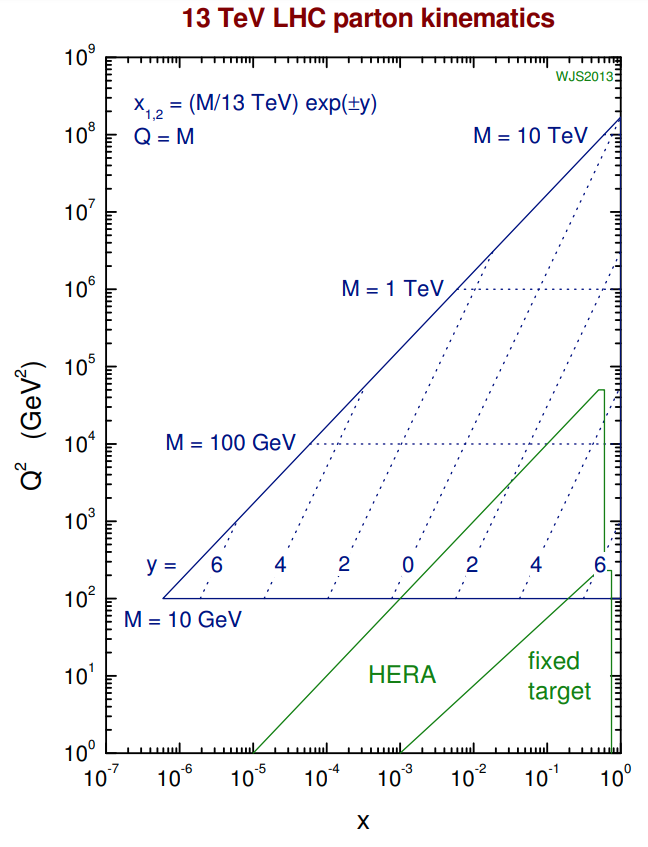
\includegraphics[width=12cm]{img/xQ2planeCoverage.png}
	\caption{Graphical representation of the parton $(x,Q^2)$ variables coverage of different experiments. For LHC these $x$ and $Q^2$ are related to the kinematic variables $y$ and $M$. Figure from \cite{StirlingPrivate}}
		\label{figure:xQ2planeCoverage}
\end{figure}

\section{Partonic cross-section}

Partonic cross section as seen in \eqRef{eq:factorization1} is one of the fundamental ingredients in our recipe for the description of hadron-hadron interactions. It can be calculated as a perturbative expansion in $\alpha_s$ from QCD first principles using quantum field theory.
\\
The calculation of such expansion at the leading order (LO) is performed by evaluating all the possible tree-level Feynman diagrams for every process. Then the calculation proceeds by computing the squared matrix element and by integrating it over the available phase space (analytically or numerically).
\\
At this point, we can already encounter some divergence that can be avoided imposing some  restrictions on the phase space.
% restriction or constraints

\subsection{Higher order calculations}

The LO calculation can describe broad feature of a particular process and provide a first estimation of its cross section; anyway, in many cases this is insufficient.
\\
The main source of uncertainty derives from the LO dependence  on the unphysical renormalization and factorization scales. Some process may contribute only when going beyond the first approximation, and some divergence can be resummed. 
\\
The next-to-leading order (NLO) calculation requires all the Feynman diagrams that take an extra $\alpha_s$. This contribution can arise in two different ways:
\begin{itemize}
	\item \textbf{Virtual}: internal lines in the Feynamn diagram, see \figRef{fig:feynman_Real_Virtual}a, that don't originate a real particle in the initial or in the final state (loops);
	\item \textbf{Real}: external lines int the Feynamn diagram, see \figRef{fig:feynman_Real_Virtual}b, here the particle is real and participate to the initial or final state observed (real particles).
\end{itemize}
\begin{figure}[!htb]
	\centering
	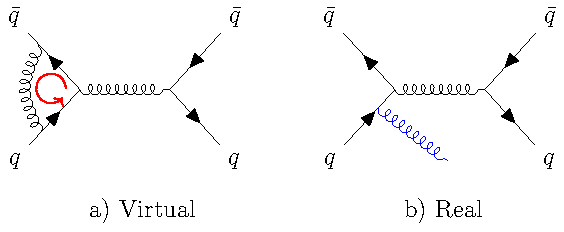
\includegraphics[width=0.7\textwidth]{img/feynman_Real_Virtual.pdf}
	\caption{Feynamn diagrams for a virtual correction (a) the momentum circulating in the loop when integrated on the phase space take to a divergence; and a real correction (b) the particle emitted is real, participate to the initial or final state of the process.}
	\label{fig:feynman_Real_Virtual}
\end{figure}

Virtual corrections contains infrared divergences, arising by integrating on the loop circulating momentum, that cancel against infrared singularities given by collinear  or soft emissions \cite{PhysRevBloch, KinoshitaToichiro, PhysRevLee}. 
\\
A common strategy for the renormalization is dimensional regularization: it consists into performing the calculation in a $D=4-2\epsilon$ dimensional space ($\epsilon<0$); in that way the singularities appear as single and double poles in $\epsilon$. Then, the limit $\epsilon\rightarrow0$ is taken after the divergences have cancelled.
\\
This NLO calculation with regularization allows to extend the treatment of these integrals up to zero transverse momentum.

The importance of higher-order calculation is that it allows too describe more processes, as can be shown with the following example. In a $Z$ boson production:
\begin{enumerate}[label=$\arabic*)$]
	\item \textbf{LO}: the $Z$ is produced without transverse momentum ($p_T$), and anything can recoil against the $Z$ for momentum conservation (\figRef{fig:Zprod_feynman_LO_NLO_NNLO}{\color{blue}{a}}). 
	\item \textbf{NLO}: the $Z$ acquires a finite $p_T$. In this case the $Z$ boson $p_T$ is balanced by a single \mbox{parton/gluon} (\figRef{fig:Zprod_feynman_LO_NLO_NNLO}{\color{blue}{b}}).
	\item  \textbf{NNLO}: the $Z$ $p_T$ can be balanced by two jets (\figRef{fig:Zprod_feynman_LO_NLO_NNLO}{\color{blue}{c}}). 
\end{enumerate}
\begin{figure}[!htb]
 \centering
 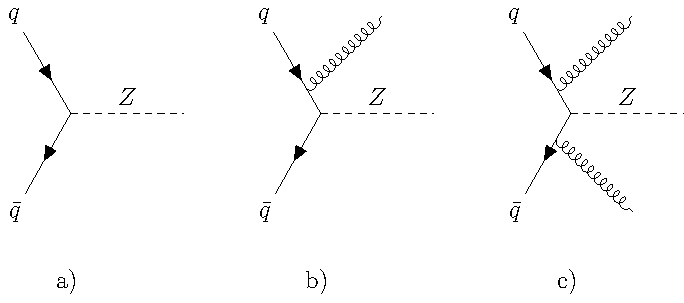
\includegraphics[width=12cm]{{img/feynman_ZpT.pdf}}
 \caption{Feynman diagrams for the Z production by annihilation of a quark and an antiquark at LO (a), NLO (b), NNLO (c). At LO the $Z$ can only be produced with a $p_T=0$ for the conservation of the momentum.}
 \label{fig:Zprod_feynman_LO_NLO_NNLO}
\end{figure}
Another important benefit of performing a NLO calculation is the the reduction of the dependence of calculation on the unphysical renormalization ($\mu_R$) and factorization ($\mu_F$) scales.
It is proven that higher order calculations of observables calculated to order $\alpha_s^{\,n}$ are dependent upon the unphysical scales only at order higher than $\alpha_s^{\,n+1}$ \cite{Campbell2006}. The range of predictions corresponding to different scale choices is usually attributed to \textit{theoretical uncertainties}, as is shown in \figRef{fig:ZRapidityDistributionLO_NLO_NNLO}, where the uncertainties reduce from the LO calculation to the NLO and even more to the NNLO.

\begin{figure}[!htb]
	\centering
	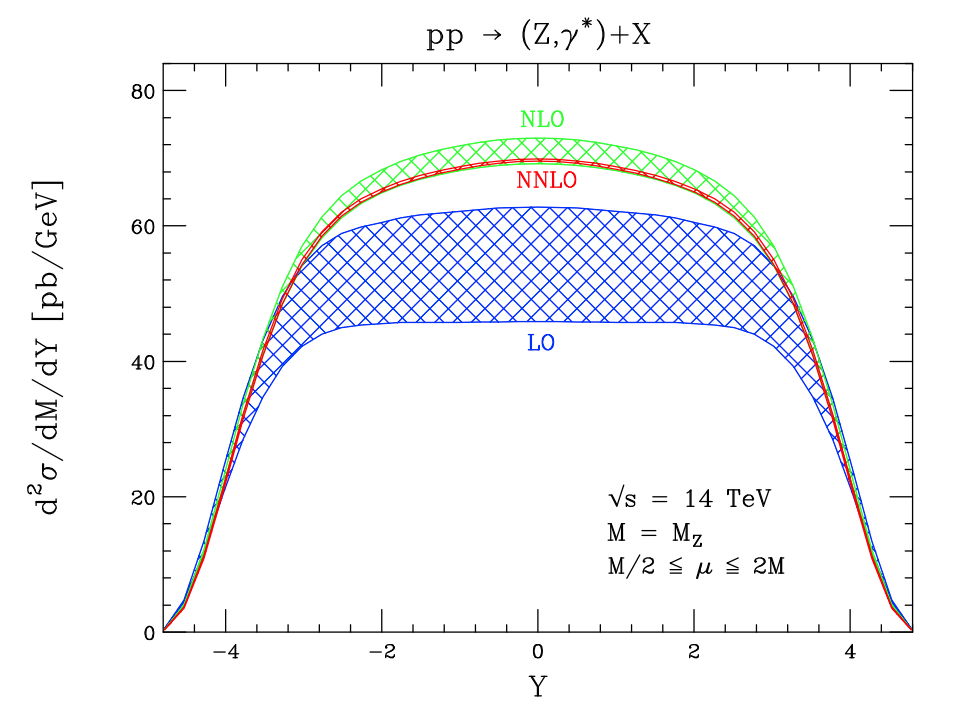
\includegraphics[width=12cm]{{img/ZRapidityDistributionLO_NLO_NNLO.png}}
	\caption{The rapidity distribution predictions at LO (blue) NLO (green) and NNLO (red) for the Z production at the center of mass energy$\sqrt{s}=14\ \mathrm{TeV}$. The band width is related to the uncertainties. Going from LO to NLO there is a increase in the cross section prediction and a reduction on the scales uncertainties, the NNLO prediction is in the NLO error band width but there is a further increase in the precision of the prediction. Figure from \cite{Campbell2006}, section 6.}
	\label{fig:ZRapidityDistributionLO_NLO_NNLO}
\end{figure}

\section{Parton Showers}

A different approach to describe the phenomena observed at high-energy colliders, instead of calculating cross sections order by order in the perturbative expansion, is the use of an \textit{all-order} approach. 
\\
Different all-order approaches exist such as resummation techniques and parton showers. Resummation is based on the observation that in many quantities the smallness of the expansion coefficients $\alpha_s$ is violated by large logarithmic enhancements. This takes the dominant contribution from each order and "resums" them by means of an evolution equation. 
The main problem in QCD is related to the fact that lot of quantities have corrections of the form $\alpha_s^n\log^k(Q_i/Q_j)$ where $Q_i$ and $Q_j$ are two different energies scales, for example:
\begin{itemize}
	\item[--] Renormalization $\mu_R=Q^2$ and factorization scales logs: $\alpha_s^n\log^n(Q^2/\mu_f)$
\end{itemize}
Various methods to perform this resummation exist.
\\
%%%% GRAPH on pT Z with effect of resummation 
An example is the $Z$ production $p_T$ spectrum shown in \figRef{figure:pT_Z_CDF}: here the comparison between experimental CDF data and theoretical predictions is shown: in the low $p_T$ region the \textit{all-order} approach regularizes the divergence of the fixed order calculation and describes the data better. 

\begin{figure}[!htb]
	\centering
	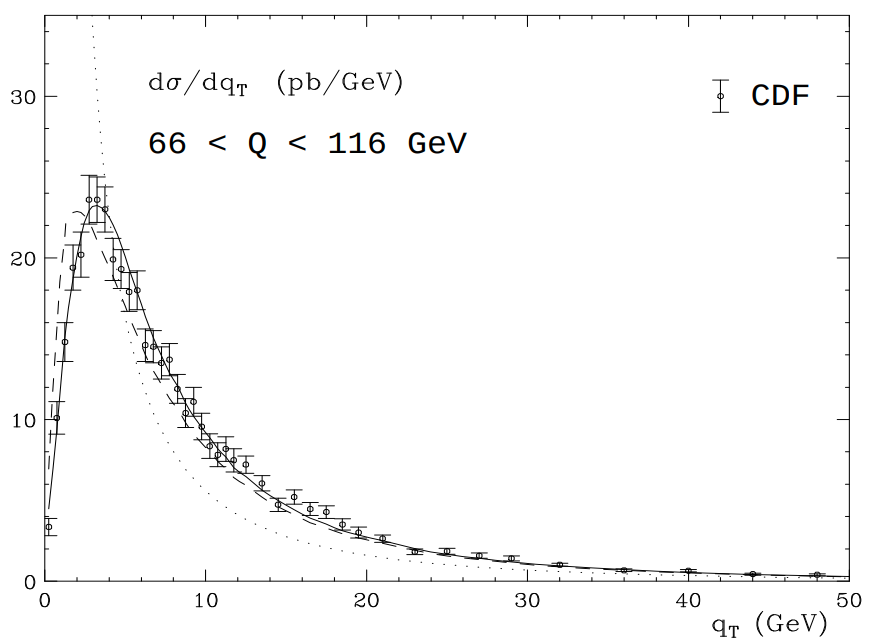
\includegraphics[width=12cm]{{img/pT_Z_CDF.png}}
	\caption{CDF data on $Z$ production cross section at Tevatron collider, CDF experiment, the predictions from fixed order calculation (dotted) with resummation (dashed), and with the inclusion of power corrections (solid) are compared. Figure take from \cite{kulesza2002electroweak}}
	\label{figure:pT_Z_CDF}
\end{figure}

An other \textit{all-order} approach is based on the simulation of the so-called "parton showers". It is  implemented in different Monte Carlo programs, as  \textsc{pythia} \cite{PYTHIA2015}, \textsc{herwig} \cite{Herwig2008} and \textsc{sherpa} \cite{SHERPA2004}. 
The algorithm starts from few partons arising from a hard interaction. Then, as the energy scale at which we examines the scattering decrease these harder partons can split, and so more partons are produced in the shower. The higher scale parton are related to the lower energy scale (close to $\Lambda_{QCD}$) using the DGLAP evolution equation formalism. The solution to this equation can be written using a Sudakov form factor arising from the probability of no gluon emission in the evolution from higher to lower scale.
\\
In the parton showering process, in addition to the kinematic variables (momentum fraction $z$ and azimuthal angle $\phi$) and flavours of the partons, an evolution variable $t$ is generated. \textsc{Pythia8} uses as  evolution variable the squared of the relative transverse momentum of the two partons in the splitting ($p_T^2$). Different choices are made in \textsc{herwig} and \textsc{sherpa}.
\\
As mentioned before, the shower evolution is based on the standard (LO) DGLAP splitting kernels P(z) described here:
\begin{align}
P_{q\,\rightarrow\,qg}(z) & = C_F\frac{1+z^2}{1-z}\quad ; \\
P_{g\,\rightarrow\,gg}(z) & = C_A\frac{(1-z(1-z))^2}{z(1-z)}\quad ; \\
P_{q\,\rightarrow\,q\overline{q}}(z) & = T_R(z^2+(1-z)^2)\quad ;
\end{align} 
where $C_F=\frac{4}{3}$ is the Casimir operator for $SU(3)$, $C_A=N_C=3$, that are named "color factors", and $T_R=\frac{1}{2}$ that is given by the trace calculation of the group generators, each contribution is multiplied by $N_f$ if summing over all contributing quark flavours.
\\
The parton shower consist of two components: the initial-state radiation (ISR) describing the emission from the incoming partons and the final-state radiation (FSR) describing emission of outgoing partons.
Both ISR and FSR algorithms are based on these splitting kernels.
The respective probabilities of emitting radiation as one moves in the decreasing evolution variable sequence are:
\begin{align}
	FSR: \qquad\quad & \frac{d\mathcal{P}_{FSR}}{dp_T^2} = \frac{1}{p_T^2}\displaystyle\int \frac{dz}{z}\,\frac{\alpha_s}{2\pi}P(z)\quad ;\label{eq:FSR1}\\
	ISR: \qquad\quad & \frac{d\mathcal{P}_{ISR}}{dp_T^2} = \frac{1}{p_T^2}\displaystyle\int \frac{dz}{z}\,\frac{\alpha_s}{2\pi}P(z)\,\frac{f'(x/z,p_T^2)}{f(x,p_T^2)}\quad .\label{eq:ISR1}
\end{align}
We can write-out our Sudakov form factor by using the two probability in \eqRef{eq:FSR1} and \eqRef{eq:ISR1}, as
\begin{equation}
	\Delta(p_T^2)=\exp\left( -\displaystyle\int_{p_T0}^{p_T'} \frac{d\mathcal{P}_{PS}}{dp_T^2} \,dp_T\right) \qquad\text{ with } \quad PS=ISR,\ FSR \quad.
	\label{eq:sudakovFormFactor}
\end{equation}
The Sudakov form factor give the probability of a parton to evolve from an harder scale to a softer scale without emitting a parton harder than some resolution scale. 
\\
The introduction of the Sudakov form factor resums all the effects from the soft and collinear gluon emission. For more details and some plots of different Sudakov form factor values see section 3.5 of \cite{Campbell2006}.

\subsection{Merging parton showers and matrix element calculations}

Regions dominated by soft and collinear gluon emissions are described very well by parton showers approach; on the other hand, regions where partons are  energetic and widely separated are well described by matrix element calculations.  
So, the best approach would be to combine the two different descriptions, this would require an universal formalism for parton showers and matrix element calculations. This universal formalism was created in 2001 and it is called "Les Houches Accord" \cite{LesHouchesAccord}.
In order to combine the two approaches some care must be taken: there is the risk of double counting. Different techniques prevent this risk: for example CKKW \cite{CKKW2001} is used to combine LO matrix element calculations and parton shower.


A better way is to combine NLO matrix element calculation with parton showers: this is done by the FxFx mergin scheme, developed by Frixione, Nason, Webber in the \textsc{mc@nlo} framework \cite{FxFx1,FxFx2,FxFx3,FxFx4}. In this scenario the risk of  double counting is given by the fact that at NLO one emission can be made explicit as indicated in \figRef{fig:DoubleCounting} by the red gluon line, then the progress of the parton shower can leads to a double counting between real emission matrix element and the parton shower as shown in \figRef{fig:DoubleCounting}, the double counting sources are indicated by the blue arrows.
% TODO: mi piacerebbe aggiungere una descrizione più completa del merging con FxFx visto che viene usato dopo. 

%%%
%%% Immagine di Frixi.. presentation
\begin{figure}[H]
	\centering
	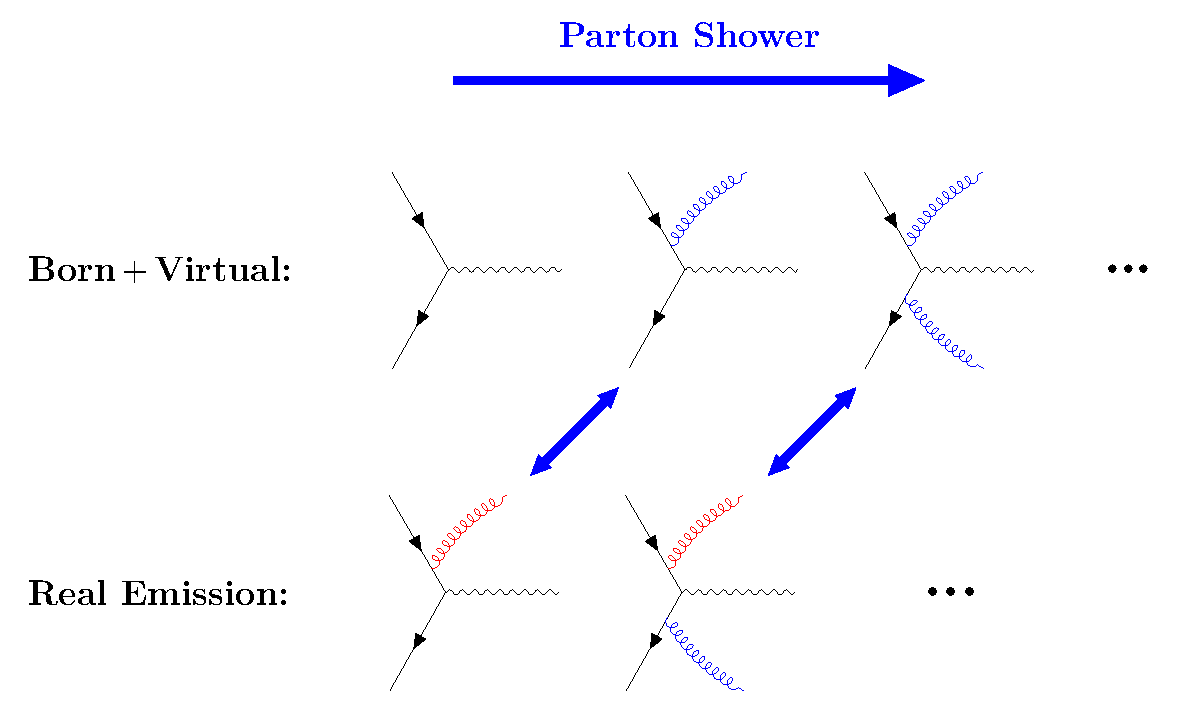
\includegraphics[width=14cm]{{img/feynman_doubleCounting_FxFx_curved-cropped.pdf}}
	%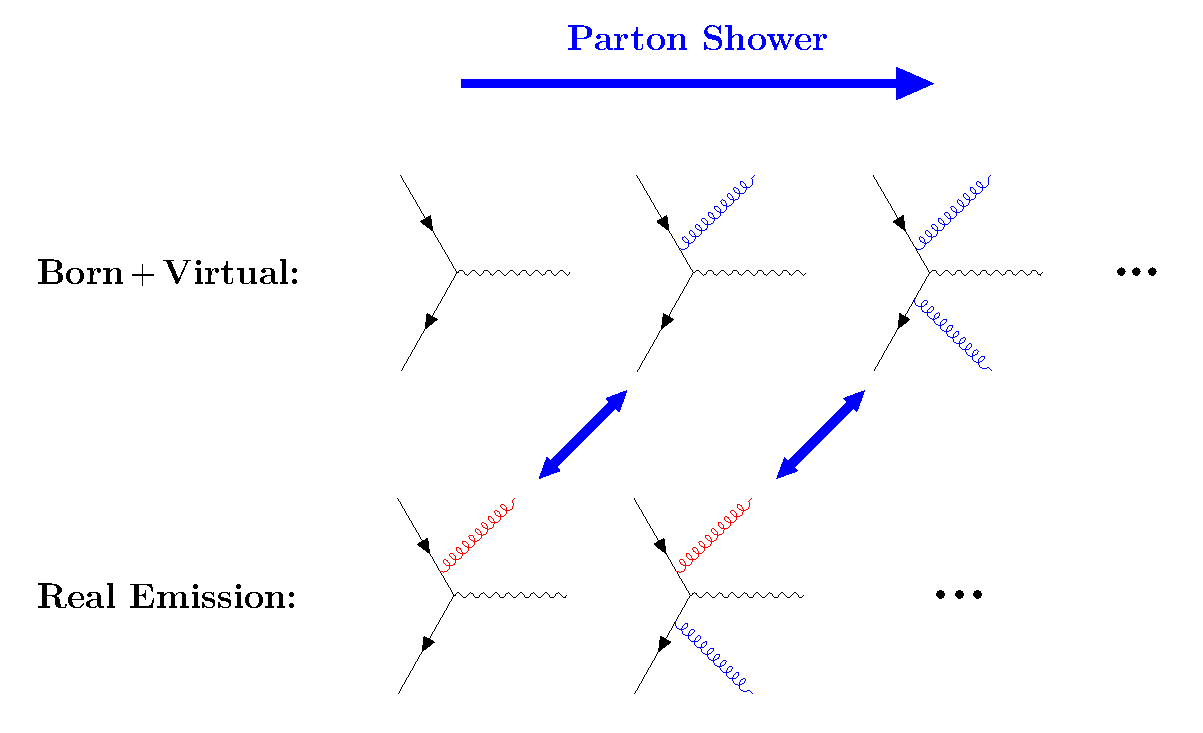
\includegraphics[width=14cm]{{img/feynman_doubleCounting_FxFx-cropped.pdf}}
	\caption{The FxFx margin scheme have to avoid this double counting. Feynman diagrams that can lead to a double counting are grouped with the violet arrow, the blue emission are related to the parton shower while the red ones to the NLO process.}
	\label{fig:DoubleCounting}
\end{figure}
%%%


\section{Parton distribution functions}

The last ingredient in our recipe is the knowledge of the quark and gluon distributions inside the two hadrons that undergo the scattering. We have already seen that these quantities are depending on the virtuality ($Q^2$) of the interaction.
\\
The information on the quark distribution inside a hadron $f_{q/p}(x,Q^2)$ arises from lepton-hadron DIS experiments, from lepton-pair production in hadron-hadron collisions (Drell-Yan processes) and jet measurements to study gluon distribution $f_{g/p}(x,Q^2)$. All these quantities are the experimental input in order to evaluate the PDF inside the hadron while the $Q$-evolution is described by DGLAP equation.
The evolution of the PDF can be run either with a NLO or with a NNLO calculations.

The kinematic region covered by experiments is shown in \figRef{figure:xQ2planeCoverage}. At very low x and $Q^2$ the DGLAP evolution is believed to be no longer applicable and a BFKL (Balitsky-Fadin-Kuraev-Lipatov) \cite{BFKL1,BFKL2} description must be used.
%;
%anyway, this has not any experimental evidence so the DGLAP approach is used as default in all the PDF analysis.
% but there are no experimental evidence of this so the DGLAP approach is used as default in all the PDF analysis.
\\
A lot of processes are available for the PDFs evaluation and a lot of PDF set have been generated, as an example \figRef{fig:NNPDF31} shows the NNPDF3.1 set \cite{NNPDF3.1} at NNLO for a virtuality $Q^2=10\ \mathrm{GeV^2}$ (left) and $Q^2=10^4\ \mathrm{GeV^2}$ (right). 
\begin{figure}[!htb]
	\centering
	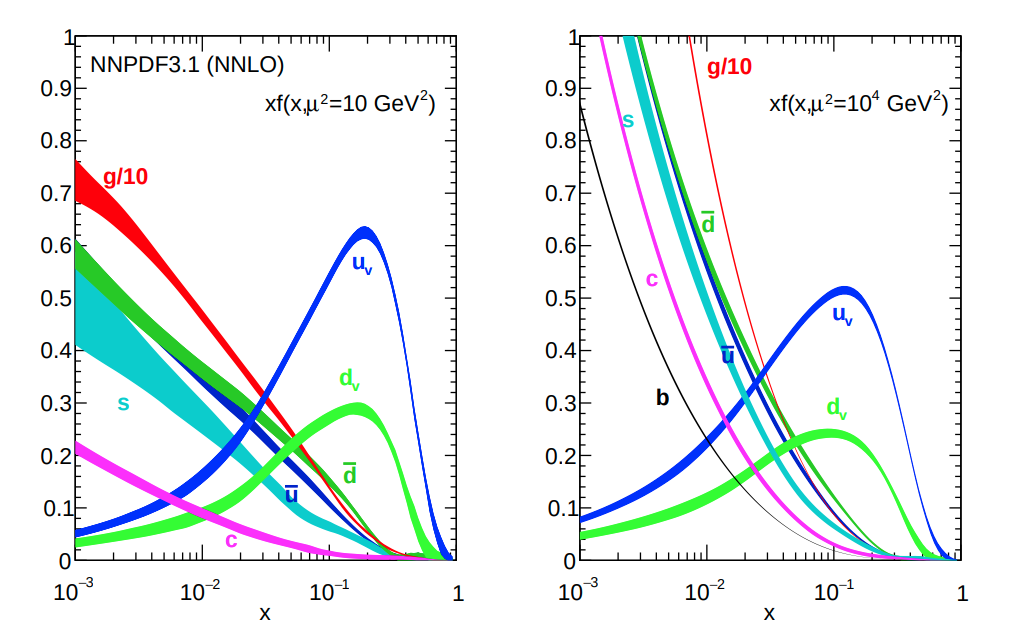
\includegraphics[width=12cm]{{img/NNPDF3.1.png}}
	\caption{The NNPDF3.1 NNLO PDFs set, evaluated at $Q^2 = 10\ \mathrm{GeV}^2$
(left) and $Q^2=10^4\ \mathrm{GeV}^2$ (right). At low $x$ the contribution from the gluons is the dominating one while at higher x the dominant contribution is from the valence quarks. The PDF $Q$ evolution shows that when our proton is probed to higher $Q^2$ the resolution increase (higher $Q$ correspond to smaller distance resolution) and so we have a bigger contribution from the sea quarks at low $x$ values.}
	\label{fig:NNPDF31}
\end{figure}
Note that the gluon contribution have been scaled of a factor 10: in fact, in the low $x$ region, $x<0.01$, the gluon contribution is the dominating one, while at high $x$ value the valence quarks dominate the PDF. 
\\
In \figRef{fig:NNPDF31} we can also see that with increasing virtuality ($Q^2$) at low $x$ the density of the sea quarks increases: this is related to the fact that our hadrons are probed at higher energy and the probe resolution is proportional to the energy. 
\begin{equation}
	\text{Resolution}\sim\frac{\hbar}{Q}\quad .
\end{equation}
So, when probed at higher energy, the hadrons appear denser than when are probed at lower energy. This, as will be discussed in the next chapter, is related to the higher number of interaction between partons in a single hadron-hadron collision. The phenomenon of having more than one interaction between partons in a single hadron-hadron collision is called \textit{multiple parton interaction}: this concept will be discussed in the next chapter.


\section{A real proton-proton collision}


We have understood that the complexity in the description of a proton-proton collision arises from composite nature of the protons. In this chapter we discussed the importance of the QCD factorization theorem that help us in the calculation of the hadronic cross section with the convolution between the partonic cross section and the PDF. We have discussed the importance of the parton shower algorithm where a set of partons are evolved in a more complex final state by emissions in the initial and final states.
\\
All these processes are important in the description of a real proton-proton collision but also the partons that are left unscattered are non-color singlet and can contribute to the complex final state observed in the experiments, and additionally, as mentioned before, nothing prevent additional partons scatterings from taking place and growing more and more the complexity of the partons final state. 

Than, another problem is related to the not-well-understood hadronization process.
Hadronization is not known from first principles and different models have been implemented in different programs: the \textit{cluster fragmentation model} implemented in \textsc{herwig} and the \textit{string fragmentation model} in \textsc{pythia} simulated this process of hadronization where the set of final-state partons is transformed into a set of hadrons. All these processes are schematically shown in \figRef{fig:Processes}.

\begin{figure}[!htb]
	\centering
	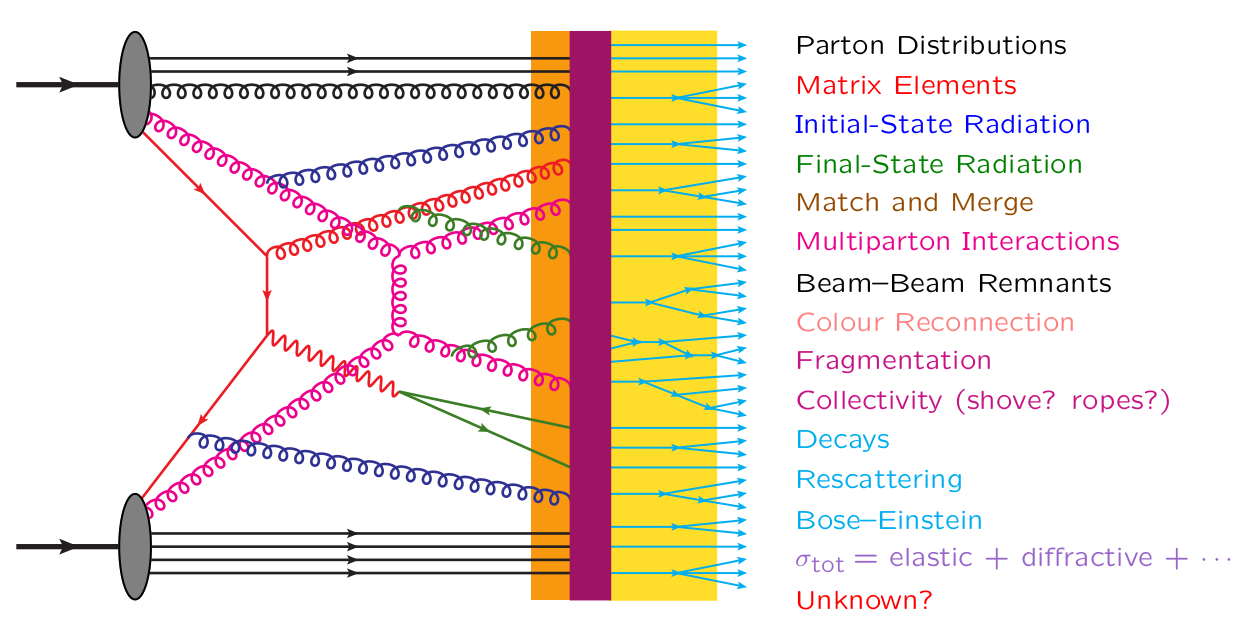
\includegraphics[width=0.98\textwidth]{{img/Processes.png}}
	\caption{A schematic representation for a $pp$ collision. Reading the image from left to right one can have an idea on the evolution of the system. The two incoming hadrons enter the scattering from the left side, the read line indicate the main hard scattering and the fuchsia one the second parton scattering (MPI) each interaction is associated with initial (blue) and final (green) state radiation, the unscattered partons (black lines) re-enter the color reconnection and hadronization processes. Than the new formed hadrons (lightblue) can undergo to different decays.}
	\label{fig:Processes}
\end{figure}

Next chapter is going to describe the \textsc{pythia} Monte Carlo generator in more details. \textsc{pythia} introduces different free parameters that need to be tuned with experimental data from Tevatron and LHC. The tune methods are described in \chapRef{chap:TuneprocedureCP5TuneandMCNNTUNES} along with the description of some already existing tune for the underlying event in proton-proton collision.



%%% ---



%In a \textbf{proton-proton collision}, additionally to the main hard scattering that can be described performing Matrix Element calculations (MEs) , also other scattering processes are possible. To well understood the proton-proton collision we need to describe other processes, besides to the hard scattering, that can underlying to this  \textbf{Multi Parton Interaction} (MPI) and the \textbf{Beam-Beam Remnants} (BBR).




%\end{document}}
	
\graphicspath{{Multi_Parton_Interactions/}}

\chapter{Multiple Parton Interactions}
\label{chap:MultiplePartonInteractions}


By the fact that the hadrons are viewed as "bunches" of partons, it is likely that in the same hadron-hadron collision different couples of partons can undergo to a scattering. This phenomenon is known as \textit{Multiple Parton Interactions} (MPI) and it is related to the composite nature of the incoming hadrons. 
\\
So, it is clear that at some level these MPI have to exist, and they can become important in the description of the event; they can change the color topology of the colliding system as a whole.  
\\
In this scenario it is important to have a good understanding of the phenomenon. The aim of this section is to describe the basic concepts that are use to simulate MPI, for example in \texttt{Pythia} Monte Carlo event generator; then some focus is given to the free parameters we are going to tune in the following sections.

\section{Basic Concepts}
\label{sec:BasicConcepts}

The main hypothesis of the multiple interactions models is that: the QCD factorization theorem is true not only for the hard process but also for the other partons scatters.
\\
So, we can write:
\begin{equation}
	\frac{d\sigma_{\text{int}}}{dp_\perp}=\displaystyle\sum_{i,j,k,l}\displaystyle\int dx_1 \displaystyle\int dx_2 \displaystyle\int d\hat{t}\, f_i(x_1,Q^2)f_j(x_2,Q^2)\frac{d\hat{\sigma}_{ij\,\rightarrow\,kl}}{d\hat{t}}\delta\left( p_\perp^2-\frac{\hat{t}\hat{u}}{\hat{s}} \right) \quad .
	\label{eq:sigma_int1}
\end{equation}
This represent the interaction differential cross section for the hadron-hadron collisions, where $\frac{d\hat{\sigma}_{ij\,\rightarrow\,kl}}{d\hat{t}}$ is the differential cross section for QCD hard $2\ \rightarrow 2$ processes, this processes are the one reported in \tableRef{table:partonic_cross_sections}. 
\\
In \eqRef{eq:sigma_int1} we used the Mandelstam variables associated to the partonic system:
\begin{align}
	&\hat{s}=(p_1+p_2)^2=(p_3+p_4)^2=x_1x_2s\\
	&\hat{t}=(p_1-p_3)^2=(p_2-p_4)^2\\
	&\hat{u}=(p_1-p_4)^2=(p_2-p_3)^2
\end{align} 
where $p_1$, $p_2$ are the four-momenta of the incoming partons and $p_3$, $p_4$ the four-momenta of the outgoing partons. 

%Note that in \eqRef{eq:sigma_int1} the jet cross section is twice as large $\sigma_{\text{jet}}=2\sigma_{\text{int}}$, because at first approximation each interaction gives rise to two jets.

\noindent We assume also that the "hardness" of processes is defined by the $p_T$ scale of the interaction ($Q^2=p_T^2$).

%\begin{table}[!ht]
%	\centering
%	\begin{tabular}{l | c}\rule{0pt}{3ex} 
%	Process & Partonic cross section \rule{0pt}{3.5ex}\\   \hline\hline 
%	$q\,q'\ \rightarrow\ q\,q'$ & $\frac{4}{9}\frac{\hat{s}^2+\hat{u}^2}{\hat{t}^2}$\rule{0pt}{3.5ex}\\
%	$q\,q\ \rightarrow\ q\,q$ & $\frac{4}{9}\left(\frac{\hat{s}^2+\hat{u}^2}{\hat{t}^2}+\frac{\hat{s}^2+\hat{t}^2}{\hat{u}^2}\right) -\frac{8}{27}\frac{\hat{s}^2}{\hat{u}\hat{t}}$\rule{0pt}{3.5ex}\\
%	$q\,\overline{q}\ \rightarrow\ q'\,\overline{q}'$ & $\frac{4}{9}\frac{\hat{s}^2+\hat{u}^2}{\hat{t}^2}$\rule{0pt}{3.5ex}\\
%	$q\,\overline{q}\ \rightarrow\ q\,\overline{q}$ & $\frac{4}{9}\left(\frac{\hat{s}^2+\hat{u}^2}{\hat{t}^2}+\frac{\hat{t}^2+\hat{u}^2}{\hat{s}^2}\right) -\frac{8}{27}\frac{\hat{u}^2}{\hat{s}\hat{t}}$\rule{0pt}{3.5ex}\\
%	$q\,\overline{q}\ \rightarrow\ g\,g$ & $\frac{32}{27}\frac{\hat{t}^2+\hat{u}^2}{\hat{t}\hat{u}}-\frac{8}{3}\frac{\hat{t}^2+\hat{u}^2}{\hat{s}^2}$\rule{0pt}{3.5ex}\\
%	$g\,g\ \rightarrow\ q\,\overline{q}$ & $\frac{1}{6}\frac{\hat{t}^2+\hat{u}^2}{\hat{t}\hat{u}}-\frac{8}{3}\frac{\hat{t}^2+\hat{u}^2}{\hat{s}^2}$\rule{0pt}{3.5ex}\\
%	$g\,q\ \rightarrow\ g\,q$ & $-\frac{4}{9}\frac{\hat{s}^2+\hat{u}^2}{\hat{s}\hat{u}}-\frac{\hat{u}^2+\hat{s}^2}{\hat{t}^2}$\rule{0pt}{3.5ex}\\
%	$g\,g\ \rightarrow\ g\,g$ & $\frac{9}{2}\left( 3-\frac{\hat{t}\hat{u}}{\hat{s}^2} -\frac{\hat{s}\hat{u}}{\hat{t}^2} - \frac{\hat{s}\hat{t}}{\hat{u}^2} \right)$\rule{0pt}{3.5ex}
%	\end{tabular}
%	\caption{Parton-Parton differential cross sections ($2\ \rightarrow\ 2$ QCD process), can beh calculated in pQCD evaluating the matrix element for each process involving quark, antiquark and gluon.}
%	\label{table:partonic_cross_sections}
%\end{table}

\begin{table}[!ht]
	\centering	
	\begin{tabular}{| c | P{6cm} | c |}
	\hline
	Process & Amplitude & $\displaystyle\sum|\mathcal{M}|^2/(4\pi\alpha_s)^2$\\\hline\hline
	$qq'\,\rightarrow\,qq' $ & \scalebox{0.95}{\raisebox{-.5\height}{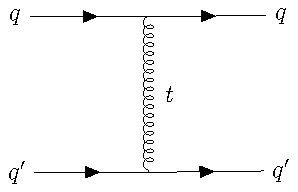
\includegraphics[width=2.5cm]{{img/DiagrammiPartonic/feynman_partonic_1.pdf}}}} & $\displaystyle{ \frac{4}{9}\frac{s^2+u^2}{t^2} }$\\\hline
	$qq\,\rightarrow\,qq $ & \scalebox{0.95}{\raisebox{-.5\height}{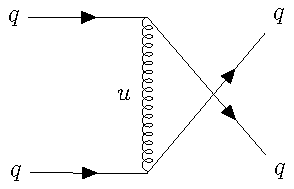
\includegraphics[width=2.5cm]{{img/DiagrammiPartonic/feynman_partonic_2.pdf}}\qquad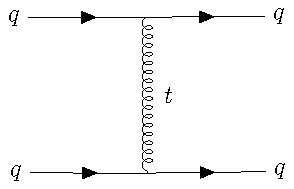
\includegraphics[width=2.5cm]{{img/DiagrammiPartonic/feynman_partonic_3.pdf}}}} & $\displaystyle{\frac{4}{9}\frac{s^2+u^2}{t^2} + \frac{4}{9}\frac{s^2+t^2}{u^2} - \frac{8}{27}\frac{s^2}{tu}}$\\\hline
	$q\overline{q}\,\rightarrow\,q'\overline{q'} $ & \scalebox{0.95}{\raisebox{-.5\height}{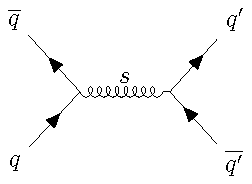
\includegraphics[width=2.5cm]{{img/DiagrammiPartonic/feynman_partonic_4.pdf}}}} & $\displaystyle{\frac{4}{9}\frac{t^2+u^2}{s^2}} $\\\hline
	$q\overline{q}\,\rightarrow\,q\overline{q} $ & \scalebox{0.95}{\raisebox{-.5\height}{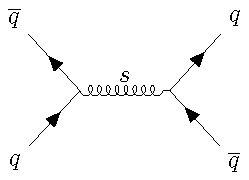
\includegraphics[width=2.5cm]{{img/DiagrammiPartonic/feynman_partonic_5.pdf}}\qquad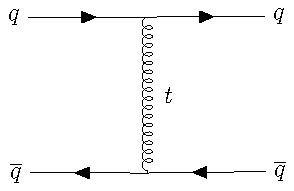
\includegraphics[width=2.5cm]{{img/DiagrammiPartonic/feynman_partonic_6.pdf}}}} & $\displaystyle{\frac{4}{9}\frac{s^2+u^2}{t^2} + \frac{4}{9}\frac{t^2+u^2}{s^2} - \frac{8}{27}\frac{u^2}{st}}$\\\hline
	$q\overline{q}\,\rightarrow\,gg $ & \scalebox{0.95}{\raisebox{0.0\height}{\vtop{\hbox{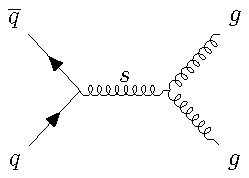
\includegraphics[width=2.5cm]{{img/DiagrammiPartonic/feynman_partonic_7.pdf}}\qquad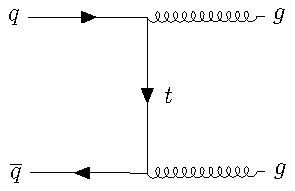
\includegraphics[width=2.5cm]{{img/DiagrammiPartonic/feynman_partonic_8.pdf}}}\begin{minipage}{4cm}{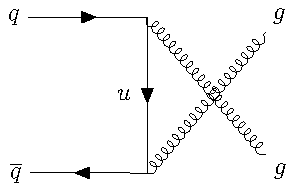
\includegraphics[width=2.5cm]{{img/DiagrammiPartonic/feynman_partonic_9.pdf}}}\end{minipage}}}} & $\displaystyle{\frac{32}{27}\frac{t^2+u^2}{tu}-\frac{8}{3}\frac{t^2+u^2}{s^2}} $\\\hline
	$gg\,\rightarrow\,q\overline{q} $ & \scalebox{0.95}{\raisebox{0.0\height}{\vtop{\hbox{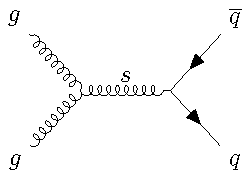
\includegraphics[width=2.5cm]{{img/DiagrammiPartonic/feynman_partonic_10.pdf}}\qquad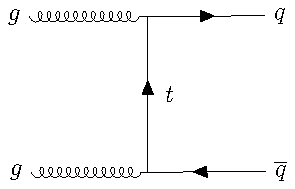
\includegraphics[width=2.5cm]{{img/DiagrammiPartonic/feynman_partonic_11.pdf}}}\begin{minipage}{4cm}{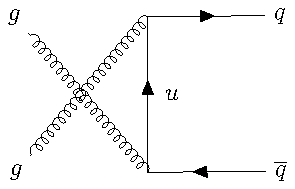
\includegraphics[width=2.5cm]{{img/DiagrammiPartonic/feynman_partonic_12.pdf}}}\end{minipage}}}} & $ \displaystyle{\frac{1}{6}\frac{t^2+u^2}{tu}-\frac{3}{8}\frac{t^2+u^2}{s^2}} $\\\hline
	$qg\,\rightarrow\,qg $ & \scalebox{0.95}{\raisebox{0.0\height}{\vtop{\hbox{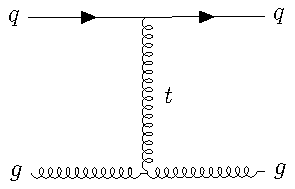
\includegraphics[width=2.5cm]{{img/DiagrammiPartonic/feynman_partonic_13.pdf}}\qquad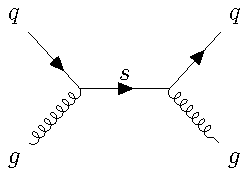
\includegraphics[width=2.5cm]{{img/DiagrammiPartonic/feynman_partonic_14.pdf}}}\begin{minipage}{4cm}{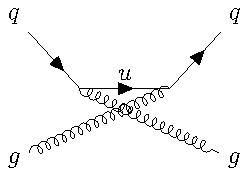
\includegraphics[width=2.5cm]{{img/DiagrammiPartonic/feynman_partonic_15.pdf}}}\end{minipage}}}} & $ \displaystyle{-\frac{4}{9}\frac{s^2+u^2}{su}+\frac{s^2+u^2}{t^2} }$\\\hline
	$gg\,\rightarrow\,gg $ & \scalebox{0.95}{\raisebox{0.1\height}{\vtop{\hbox{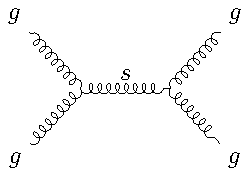
\includegraphics[width=2.5cm]{{img/DiagrammiPartonic/feynman_partonic_16.pdf}}\qquad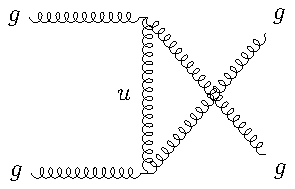
\includegraphics[width=2.5cm]{{img/DiagrammiPartonic/feynman_partonic_17.pdf}}}\hbox{\raisebox{0.1\height}{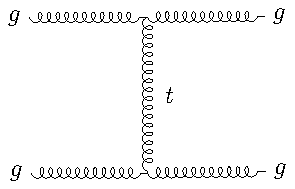
\includegraphics[width=2.5cm]{{img/DiagrammiPartonic/feynman_partonic_18.pdf}}\qquad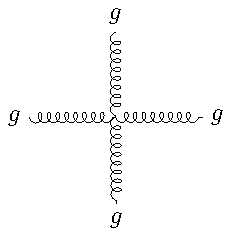
\includegraphics[width=2.5cm]{{img/DiagrammiPartonic/feynman_partonic_19.pdf}}}}}}} & $ \displaystyle{\frac{9}{2}\left( 3-\frac{tu}{s^2}-\frac{su}{t^2}-\frac{st}{u^2}\right)} $\\\hline
	\end{tabular}
	\caption{Parton-Parton differential cross sections ($2\ \rightarrow\ 2$ QCD process), can beh calculated in pQCD evaluating the matrix element for each process involving quark, antiquark and gluon. Table from \cite{SIEGERTthesis}}
	\label{table:partonic_cross_sections}
\end{table}

%\begin{table}[!ht]
%	\centering
%	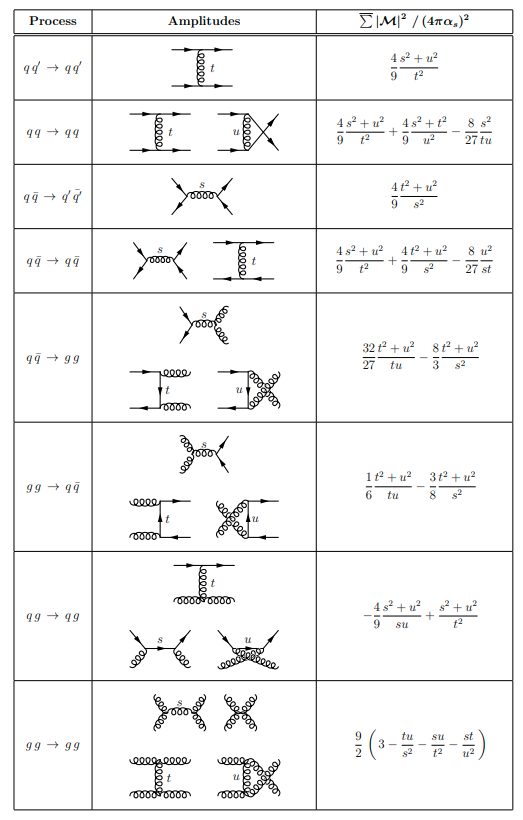
\includegraphics[width=0.8\textwidth]{{img/Table_cross_sections.png}}
%	\caption{Parton-Parton differential cross sections ($2\ \rightarrow\ 2$ QCD process), can beh calculated in pQCD evaluating the matrix element for each process involving quark, antiquark and gluon. Table from \cite{SIEGERTthesis}}
%	\label{table:partonic_cross_sections}
%\end{table}

\noindent As you can see from the formulae in \tableRef{table:partonic_cross_sections}
at small scattering angles, for $t\,\rightarrow\,0$,  the t-channel gluon exchange processes $qq'\,\rightarrow\,qq'$, $qg\,\rightarrow\,qg$ and $gg\,\rightarrow\,gg$ dominate the full matrix element. For scatterings that are soft relative to $\hat{s}$, $|\hat{t}|\ll \hat{s}$, we can approximate $|\hat{t}|$ as:
\begin{equation}
	p_T^2=\frac{\hat{t}\hat{u}}{\hat{s}} = \frac{\hat{t}(-\hat{s}-\hat{t})}{\hat{s}} \approx |\hat{t}|\quad ,
\end{equation}
in this limit, the only differences between quark and gluon cross sections are the color factors
\begin{equation}
	\hat{\sigma}_{gg}:\hat{\sigma}_{qg}:\hat{\sigma}_{qq}=\frac{9}{4}:1:\frac{4}{9}\quad .
\end{equation}
So, the \eqRef{eq:sigma_int1} can be rewritten like
\begin{equation}
	\frac{d\sigma_{int}}{dp_T^2}\approx\int\int\frac{dx_1}{x_1}\,\frac{dx_2}{x_2}\,F(x_1,p_T^2)\,F(x_2,p_T^2)\frac{d\hat{\sigma}_{2\,\rightarrow\,2}}{dp_T^2}\quad ,
	\label{eq:sigma_int2}
\end{equation}
whit:
	\begin{gather}
		\frac{d\hat{\sigma}_{2\,\rightarrow\,2}}{dp_T^2} = \frac{8\pi\alpha_s^2(p_T^2)}{9p_T^4}\quad ;\\
		F(x,Q^2)=\displaystyle\sum_q\left( x\,q(x,Q^2) + x\,\overline{q}(x,Q^2) \right) + \frac{9}{4}\,x\,g(x,Q^2)\quad .
	\end{gather}
Now, we can integrate the \eqRef{eq:sigma_int2}:
\begin{equation}
	\sigma_{int}(p_{T\,min})= \displaystyle\int_{ p_{T\,min}^2}^{(\sqrt{s}/2)^2}\frac{d\hat{\sigma}_{2\,\rightarrow\,2}}{dp_T^2}\,dp_T^2\propto \frac{1}{p_{T\,min}^2}\  \xrightarrow{\ \ p_{T\,min}\,\rightarrow\, 0 \ }\ \ \infty
	\label{eq:interaction_crossSection}
\end{equation}

\begin{figure}[!ht]
	\centering
	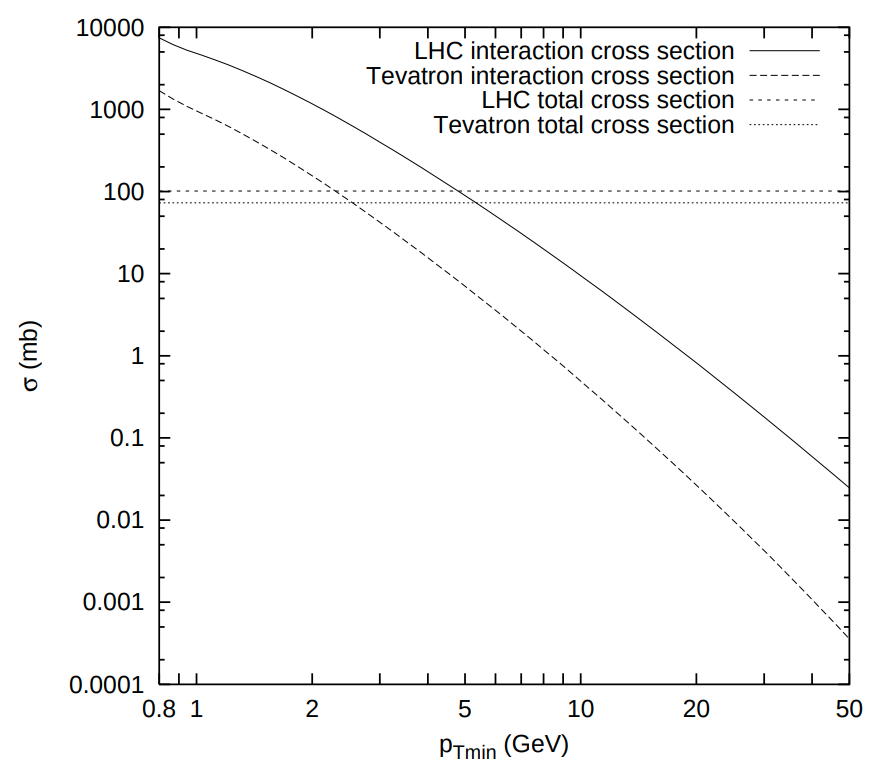
\includegraphics[width=12cm]{{img/CrossSection_Tot.png}}
	\caption{This figure shows the interaction cross section ($\sigma_{\text{int}}$) at Tevatron ($p\overline{p}$, $\sqrt{s}=1.8\ \mathrm{TeV}$) and at LHC ($pp$, $\sqrt{s}=14\ \mathrm{TeV}$). The flat lines are the corresponding values for the total cross section. The interaction cross section that arise from \eqRef{eq:interaction_crossSection} is divergent for $p_{T\,min}\,\rightarrow\,0$ in reality a dumping of this divergence is expected due to the color screening effect.}
	\label{fig:CrossSection_Tot}
\end{figure}

\noindent The total cross section is divergent in the limit $p_T\,\rightarrow\,0$, this divergence is shown in \figRef{fig:CrossSection_Tot}. Due to this divergence the total interaction cross section at some $p_{T}$ scale can exceed the total proton-proton cross section.
\\
To understand this paradox should be noted that the interaction cross section described in \eqRef{eq:interaction_crossSection} is related to the interaction probability between two partons and counts the number of interactions, while the total proton-proton cross section $\sigma_{pp}$ counts the number of events. For example, an event (a proton-proton collision) in which two partons interact counts once in the total cross section and twice in the interaction cross section.
\\
So, the ratio between this two quantities is perfectly allowed to be larger than unity, we can write it down as:
\begin{equation}
	\frac{\sigma_{int}(p_{T\,min})}{\sigma_{tot}}=\langle n \rangle (p_{T\,min})\quad .
\end{equation}
Furthermore, we have to consider the \textit{screening effect}: in fact the incoming hadrons are color singlet objects. Therefore, when the $p_T$ of an exchanged gluon is small, and so the associated wavelength large, this gluon cannot longer resolve the color charges and the effective coupling is decreased, this screening set a cutoff in the divergence. The screening effect is schematically shown in \figRef{fig:ScreeningEffect}.

\begin{figure}[!ht]
	\centering
	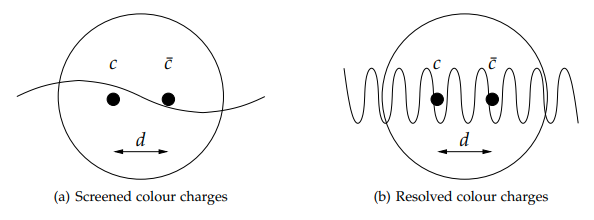
\includegraphics[width=0.7\textwidth]{{img/ScreeningEffect.png}}
	\caption{A picture of the screening effect. The left figure show two color charge that are not resolved by the gluon in fact the wave length is greater than the spatial separation, $d$, of the two charges. So resolution of the probe is not enough to discriminate the color charges. While on the right figure the two charges are very well distinct.}
	\label{fig:ScreeningEffect}
\end{figure}

\noindent So, this cutoff is associated with color screening distance i.e. the average size of the region within the  compensation of color charge occurs.
This cutoff is then introduced in the factor as:
\begin{equation}
	\frac{\alpha_s^2\,(p_{T0}^2+p_{T}^2)}{\alpha_s^2\,(p_T^2)}\,\frac{p_T^4}{(p_{T0}^2+p_T^2)^2}\quad .
\end{equation}
This factor contains the phenomenological regularization of the divergence, with the factor $p_{T0}$ that have to be tuned to data. 
\\
Now the interaction cross section is smoothly regularized and therefore finite.
\\
To be notice that: parameter $p_{T0}$ do not have to be energy-independent, but since the energy is related with the sensibility of our probe, higher energy is related with the capacity of probing PDFs to lower x values (as discussed previously, see \figRef{fig:NNPDF31}) and in this low x region the number of partons rapidly increases. So, the partons are closer packed in this regions and as a consequence the color screening distance decrease.
\\
The number of partons is related to $x$ with a power low so, it is likely to have a dependence of the same form for $p_{T0}$ respect to the center-of-mass energy
\begin{equation}
	p_{T0}(\sqrt{s})=p_{T0}^{ref} \,\left( \frac{\sqrt{s}}{E_{CM}^{ref}} \right)^{E_{CM}^{pow}}\quad .
\end{equation}
In the next section we are going to discuss how this and other effects fit into the Monte Carlo generator \texttt{pythia8}.	
	
\section{\texttt{Pythia8} Monte Carlo events generator}	

\texttt{Pythia}8 is a standard tool for the simulation of events in high energy collisions. \texttt{Pythia} contains the evolution from a few-body system to a complex multiparticles final state.

\subsection{Parton Shower}

 In \texttt{Pythia}8 all the contributions from Initial State Radiation (ISR), Final State Radiation (FSR) and Multi Parton Interactions (MPI) are interleaved into a single common sequence of decreasing $p_T$. 
\\
The parton shower has been described in the previously section. The solution to the DGLAP equation is given putting \eqRef{eq:FSR1} and \eqRef{eq:ISR1} in \eqRef{eq:sudakovFormFactor} for the ISR and the FSR by a Sudakov form factor that is related to the no emission probability in the $p_T$-evolution. 
\\
The evolution variables for ISR and FSR are defined starting from the virtuality ($Q^2$) of the emission:
\begin{equation}
	p_T^2=\left\{\begin{aligned}
		&(1-z)Q^2 && ISR\\
		&z(1-z)Q^2 && FSR
	\end{aligned}\right.\quad,
	\label{eq:partonShowerEvolutionVariables}
\end{equation}
so, in the two cases: for the FSR $Q^2_{FSR}=(p^2-m_0^2)$ in fact a time-like virtuality ($p^2>0$) is implicated, while for the ISR we have $Q^2_{ISR}=(-p^2+m_0^2)$ with a space-like virtuality ($p^2<0$). In both case $Q^2$ values are positive defined. Than the actual strong of the radiation is set by the choices of $\alpha_{s\,ISR}$ and $\alpha_{s\,FSR}$ values.

\subsection{Multiple Parton Interactions in \texttt{Pythia}}

The MPI, as said before, are also generated in a decreasing $p_T$ sequence. So the hardest MPI is generated first. Than we can write the probability for an interaction, $i$, to occur at a scale $p_T$ using a Sudakov-type expression (as we have done for the ISR and the FSR):
\begin{equation}
	\frac{d\mathcal{P}_{MPI}}{dp_T}=\frac{1}{\sigma_{ND}}\frac{d\sigma_{2\,\rightarrow\,2}}{dp_T}\ \exp\left( -\displaystyle\int_{p_T}^{p_T\,i-1} \frac{1}{\sigma_{ND}}\frac{d\sigma_{2\,\rightarrow\,2}}{dp_T'}\,dp_T' \right)\quad .
\end{equation}


\subsection{Momentum and flavour conservation}

One problem is to achieve momentum conservation, so we need to take into account the modification in the PDF by the $i-1$ interaction. To do that in \texttt{Pythia} the PDF are rescaled to the remaining available $x$ range, adjusting their normalization.
\\
We need to take into account the momentum fraction $x_i$ removed from the hadron remnant by the $i-th$ interaction. This is done evaluating PDF not at $x_i$ but at a rescaled value
\begin{equation}
	x_i'=\frac{x_i}{X} \qquad \ \text{with }\ \ X=1-\sum_{j=1}^{i-1}x_j\quad .
\end{equation}
So, using these quantities, we can rewrite our PDFs as:
\begin{equation}
	f_i(x,Q^2)\ \longrightarrow\ \frac{1}{X}f_0\left(\frac{x}{X}\right)\quad ,
\end{equation}
where $f_0$ is the original one-parton inclusive PDFs.
\\
Now, requiring also the flavour conservation and taking into account the number of valence and/or sea quarks involved in the preceding MPI. We have now the full forms of the PDFs used for the $i-th$ MPI:
\begin{align}
f_i(x,Q^2) =&  \frac{N_{fv}}{N_{fv0}}\frac{1}{X} f_{v0}\left( \frac{x}{X},Q^2 \right) + \frac{a}{X}f_{s0}\left( \frac{x}{X},Q^2 \right)+\displaystyle\sum_j \frac{1}{X} f_{c_j0}\left( \frac{x}{X},Q^2 \right) \quad,\\
g_i(x,Q^2) =& \frac{a}{X}g_0\left( \frac{x}{X},Q^2 \right)\quad, 
\end{align}
where: 
\begin{itemize}
	\item $f_i(x,Q^2)$ $(g_i(x,Q^2))$ are the squeezed PDFs for quarks (gluons);
	\item $N_{fv}$ the number of remaining valence quarks of the given flavour;
	\item $N_{fv0}$ the number of original valence quarks of the given flavour (for the proton we have $N_u=2$, $N_d=1$);
	\item $f_{s0}$ the sea-quark PDF;
	\item $f_{cj}$ the companion PDF, this arise from the splitting $g\,\rightarrow\,q\overline{q}$ and a quark $j$ is kicked out.
\end{itemize}
The factor $a$ is defined to satisfy the total momentum sum rule.

\subsection{Impact Parameter Dependence}

The simplest hypothesis for the multiple interaction simulation, it is to assume the same initial state for all hadron collisions without dependencies on the impact parameter. 
\\
The more realistic scenario it is to include the possibility that each collision could be characterized by a different impact parameter $b$, where a small $b$ value correspond to a large overlap between the two hadrons this is related to the probability of parton-parton interaction to take place.
\\
To include the impact parameter dependence on the collision, it is necessary to make some assumption on the matter distribution inside the proton. A possibility is to assume a spherically symmetric distribution inside an hadron at rest $\rho(\mathbf{x})\,d^3x=\rho(r)\,d^3x$. A Gaussian ansatz is the most simple choice but it appears to lead to a narrow multiplicity distribution and a too little pedestal effect. So the coiche is a double Gaussian:
\begin{equation}
	\rho(r) \propto \frac{1-\beta}{a_1^3}\exp\left\{-\frac{r^2}{a_1^2}\right\}+\frac{\beta}{a_2^3}\exp\left\{ -\frac{r^2}{a_2^2} \right\}\quad,
	\label{eq:matterDistribution}
\end{equation}
where a fraction $\beta$ of matter is contained in a radius $a_2$, and the rest in a larger radius $a_1$.

\medskip

Now, for a given matter distribution $\rho(r)$,  the time-integrated overlap function of the incoming hadrons during the collision is given by:
\begin{equation}
	\mathcal{O}(b)=\displaystyle\int dt \displaystyle\int d^3x\,\rho(x,y,z)\,\rho(x+b,y,z+t)\quad.
	\label{eq:overlappingFunction}
\end{equation} 
Assuming the matter distribution function in \eqRef{eq:matterDistribution} and inserting it into \eqRef{eq:overlappingFunction} we get  the following expression.
\begin{equation}
\small{
	\mathcal{O}(b)\propto \frac{(1-\beta)^2}{2a_1^2}\exp\left\{-\frac{b^2}{2a_1^2}\right\}+\frac{2\beta(1-\beta)}{a_1^2+a_2^2}\exp\left\{ -\frac{b^2}{a_1^2+a_2^2} \right\}+\frac{\beta^2}{2a_2^2}\exp\left\{-\frac{b^2}{2a_2^2}\right\}
	}
\end{equation}
this is useful to quantify the effect of overlapping protons.
The larger is $\mathcal{O}(b)$ the more probable are parton-parton scatters between the incoming protons $\langle \widetilde{n} \rangle\propto \mathcal{O}(b)$.

\medskip

So, these assumption change the so-far Poissonian nature of the framework\footnote{the Poissonian distribution, in \eqRef{eq:poisson} describe the probability of having $n$ interactions at each impact parameter. If the matter distribution have an infinite tail (like our in \eqRef{eq:matterDistribution}) events may be obtained with arbitrarily large b values. This can be a problem for the definition of the total hadron-hadron cross section}
\begin{equation}
\mathcal{P}(\widetilde{n})=
	\left\langle \widetilde{n}\right\rangle ^{\widetilde{n}}\ \frac{e^{-\langle\widetilde{n}\rangle}}{\widetilde{n}!}
	\label{eq:poisson}
\end{equation}
Now the request that at least one parton interactions in the hadron-hadron collision, ensures that we get a finite total cross section. So the probability that an event is produced by two hadrons scattering with impact parameter $b$:
\begin{equation}
	\mathcal{P}_{\text{int}}= \displaystyle\sum_{\widetilde{n}=1}^\infty\mathcal{P}_{\widetilde{n}(b)}=1-\mathcal{P}_0=1-e^{-\langle \widetilde{n}(b) \rangle}=1-e^{-k\mathcal{O}(b)}
\end{equation}
So we have now that the number of interaction per event is give by (for impact parameter $b$):
\begin{equation}
	\langle n(b) \rangle=\frac{\langle \widetilde{n}(b) \rangle}{\mathcal{P}_{\text{int}}}
\end{equation}
so, this have modified the probability distribution of interactions number from a Poissonian to a narrower one at each $b$ fixed.

\subsection{Parton rescattering}

It is not necessary that the partons undergoing to a MPI are a different partons couple from the one scattered before. As shown in \figRef{fig:Rescattering} MPI can also arise when a parton scatters more than once against partons from the other beam, this is call \textit{parton rescattering}.
%
\begin{figure}[!ht]
	\centering
	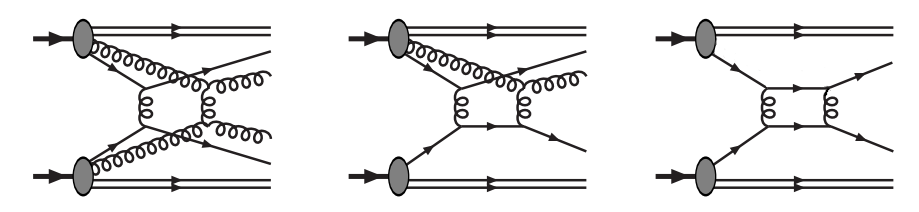
\includegraphics[width=0.95\textwidth]{{img/Rescattering_3casi.png}}
	\caption{This figure shows parton rescattering. On the right image a double $2\,\rightarrow\,2$ scattering (no rescattering) is shown; on the middle a parton rescattering process where only one of the rescattered partons have already scattered; on the right image a parton rescattering with both the partons that undergo to rescattering have already been scattered. }
	\label{fig:Rescattering}
\end{figure}
%
\\
We can have 3 type of MPI:
\begin{enumerate}
	\item No ones of the partons that enter in the second scattering undergoes to another scatter before (\figRef{fig:Rescattering} left);
	\item Only one of the two partons has alredy been scattered (\figRef{fig:Rescattering} middle);
	\item Both the partons have alredy been scattered before (\figRef{fig:Rescattering} right). 
\end{enumerate}
The second and the third are the rescatters the overall influence of rescatters in proton-proton interactions was estimated to be small respect to the first case with distinct $2\,\rightarrow\,2$  scatters. 

The simulation of parton rescatters start from the evaluation of the parton density as:
\begin{equation}
	f(x,Q^2)\ \  \longrightarrow\! \underbrace{\phantom{\Bigg(} f_{\text{rescaled}}(x,Q^2)}_{\text{hadron remnant}}+\underbrace{\displaystyle\sum_n \,\delta(x-x_n)}_{\text{scattered parton(s)}}\quad,
\end{equation} 
where the $\delta(x-x_i)$ takes into account the already scattered partons that have a fixed momentum fraction $x_n$. While the hadron remnant is still described by a continuous momentum density, scaled to achieve momentum conservation:
\begin{equation}	\displaystyle\int_0^1 \bigg( f_{\text{rescaled}}(x,Q^2) +\displaystyle\sum_n \,\delta(x-x_n) \bigg)dx=1\quad.
\end{equation}

\subsection{Interleaving of Multiple Interaction and Parton Shower}

As discussed above the MPI are simulated in \texttt{Pythia} following a decreasing $p_T$ evolution.
So we have that the total probability is given from the composition of the various contributions:
\begin{align}
	\frac{d\mathcal{P}}{dp_T}=&\left( \frac{d\mathcal{P}_{MPI}}{dp_T}+\displaystyle\sum\frac{d\mathcal{P}_{ISR}}{dp_T}+\displaystyle\sum\frac{d\mathcal{P}_{FSR}}{dp_T} \right) \nonumber \times\\ 
	&\times\exp\left\{ -\displaystyle\int_{p_T}^{p_T\,i-1} \left( \frac{d\mathcal{P}_{MPI}}{dp_T'}+\displaystyle\sum\frac{d\mathcal{P}_{ISR}}{dp_T'}+\displaystyle\sum\frac{d\mathcal{P}_{FSR}}{dp_T'} \right)\,dp_T' \right\}
	\label{eq:common_pT_sequence}
\end{align}
%
\begin{figure}[!ht]
	\centering
	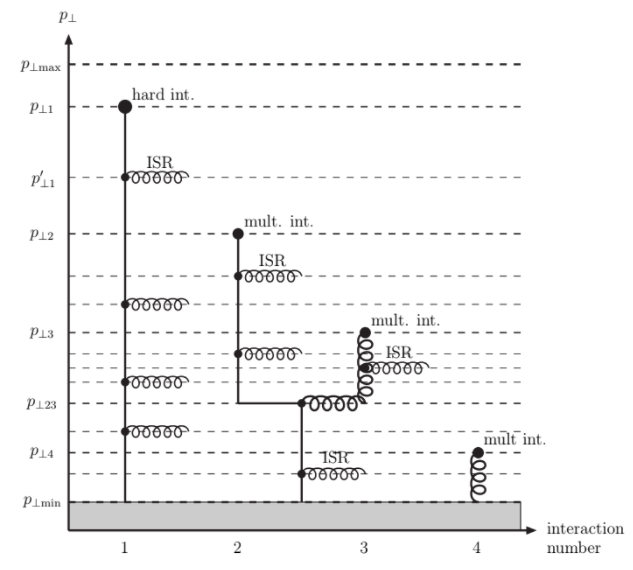
\includegraphics[width=12cm]{{img/PartonShower.png}}
	\caption{An example of Multiple Partons Interactions and associated radiations. The downward evolution in $p_T$ is shown here by reading the graph from top to bottom. The 4 parton-parton interactions occur to $p_{T1}$, $p_{T2}$, $p_{T3}$ and $p_{T4}$.}
	\label{fig:PartonShower}
\end{figure}
%
\\
In \figRef{fig:PartonShower} are shown 4 parton-parton interactions with their associated showers (ISR and FSR). The downward evolution correspond to read the graph from top to bottom. The first hard interaction occurs at a scale $p_T=p_{T1}$ while the following ones at lower scales $p_{T2}$, $p_{T3}$, $p_{T4}$. Each interaction is associated with is radiation the first one occurs at $p_T=p_{T1}'$.
The scatterings at $p_{T2}$ and $p_{T3}$ are originating from the same mother parton. 
\\
This diagram is related to one of the two hadrons. The full event can be illustrated if a similar diagram is drawn for the other hadron and connected to the full black circles.

\subsection{Beam Beam Remnants and primordial $k_T$}
\label{sec:Beam Beam Remnants and primordial kT}

What is left after that the evolution is end?
\\
The evolution in $p_T$ can create an arbitrary complicate final state. 
This final state contains contributions from the scattered and unscattered partons that don't enter the $p_T$ evolution. The last are the so called \textit{Beam Beam Remnants} (BBR). 
BBR take into account the number of valence quarks remaining and the number of sea quarks required for the overall flavour conservation.
\\
To ensure momentum conservation the BBR have to take all the remaining longitudinal momentum that is not extracted by the MPI initiators.

\subsubsection*{Primordial $k_T$}

We have considered only the longitudinal momentum. In a real scenario partons, inside the hadrons, are fermions. So, are expected to have a non zero initial transverse momentum arising from the Fermi motion inside the incoming hadrons. This is denoted as \textit{primordial $k_T$}. This is different from the transverse momentum derived from DGLAP shower evolution or from the hard interaction.

\bigskip

\noindent Based on Fermi motion alone, one would expect a value of the primordial $k_T$ of the order of: 
\begin{equation}
	k_T\simeq\frac{\hbar}{r_p}\approx\frac{0.2\ \mathrm{GeV\cdot fm}}{0.7\ \mathrm{fm}}\approx0.3\ \mathrm{GeV}\quad,
\label{eq:PrimordialKT}
\end{equation}
but, as an example, to reproduce the data for the $p_T$ distributions of $Z$ bosons produced in hadron–hadron collisions, one need a larger contribution. This phenomenon has not a satisfactory phenomenological explanation. Until a convincing explanation is found the idea is to consider an effective primordial $k_T$ for the initiators larger than the one in \eqRef{eq:PrimordialKT}.

\medskip

In \texttt{Pythia} the primordial kT is assigned to initiators sampling a Gaussian distributions for $p_x$ and $p_y$ independently with variable width $\sigma$
\begin{equation}
	\sigma(Q,\widehat{m})=\frac{Q_{1/2}\,\sigma_{\text{soft}}+Q\,\sigma_{\text{soft}}}{Q_{1/2}+Q}\,\frac{\widehat{m}}{\widehat{m}_{1/2}+\widehat{m}}
\end{equation}
Where $Q$ is the hard-process renormalization scale for the main hard process and the $p_T$ scale for subsequent MPI. $\sigma_{\text{soft}}$, $\sigma_{\text{hard}}$ are the minimum and maximum width, $\widehat{m}$ is the invariant mass, while $Q_{1/2}$ and $\widehat{m}_{1/2}$ the halfway values between the two extremes.

\subsection{Color Reconnection and Hadronization }

The last important step at parton level is the \textit{color reconnection}. Color reconnection is motivated by the fact that MPI leads to different color strings. In the previous steps the planar limit of the QCD was assumed where $N_c\rightarrow\infty$. Now, moving to real case where $N_c=3$ all this strings that can be overlapped in physical space can be reconnected. The basic idea is to reconnect strings in order to reduce the total string length; and thus the potential energy (Lund Model).
\\
In \textsc{pythia8} the reconnection is performed giving to each system a probability to reconnect given by:
\begin{equation}
	\mathcal{P}_{\text{rec}}=\frac{p_{T\,\text{rec}}^2}{\left(p_{T\,\text{rec}}^2 + p_T^2\right)} \qquad\quad p_{T\,\text{rec}}=R\times p_{T\,0}\quad,
\end{equation} 
the \texttt{ColorReconnection:range} $R$ is a user-tunable parameter while $p_{T\,0}$ is the same parameter defined in MPI simulation.
\\
With this definition for the probability, it is clear that system with low $p_T$ are more likely reconnected to other. This idea find is justification in the fact that lower $p_T$ values correspond to larger spatial extension and so these strings have more chance to overlap with other and so to reconnect.

\subsubsection*{Hadronization}

The hadronization takes all these partons (color strings) and transforms them in a set of color-neutral hadrons. Hadronization is based solely on the \textit{Lund string fragmentation model} \cite{ANDERSSON198331, Sjostrand:1984ic}. 
\\
Lund model basic idea is to break the color line and to reduce the total string length, the string is representative of the potential
\begin{equation}
	V(r)=-\frac{a}{r}+\kappa r \qquad\qquad \text{with}\quad \kappa\approx1\ \mathrm{GeV/fm}\quad,
\end{equation}
where $\kappa$ is the string tension.  This potential is a combination of an attractive (Coulomb) potential ad a linear potential that phenomenologically include quarks confinement. The linear potential is the dominating part at increasing distance values, so the energy increase with distance. 
\\
The simplest case is the one in \figRef{fig:StringBreakings}: The $q\overline{q}$ system evolves in space increasing the string length at some point the distance is to large and is convenient to break the string into two strings.

\begin{figure}[!ht]
	\centering
	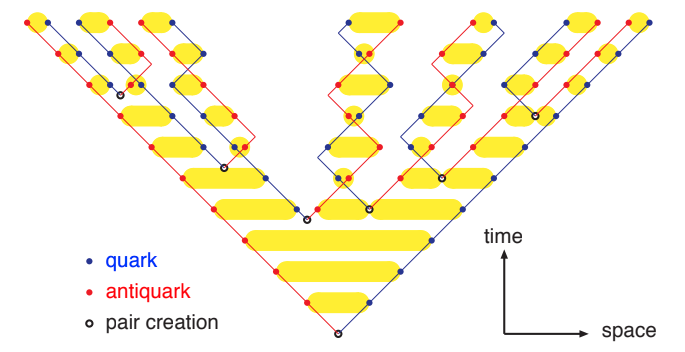
\includegraphics[width=12cm]{{img/StringBreakings.png}}
	\caption{The lund Model is schematically shown here. The string evolution in time is shown vertically while the spatial position horizontally. As the partons move apart at some point become convenient to break the string, in order to reduce the total potential energy, and a partons pair is produced.}
	\label{fig:StringBreakings}
\end{figure}

%So the hadronization try to reduce the string length.
%\begin{equation}
%	V(r)=-\frac{a}{r}+\kappa r \qquad\qquad \text{with}\quad \kappa\approx1\ \mathrm{GeV/fm}
%\end{equation}
The hadronization step confines the quark into hadrons, then these hadrons can undergoes to hadron rescattering and decay. These are the hadrons that are revealed by the detectors.

\section{\textsc{pythia} summary}

To summarize \textsc{pythia8} is able to simulate high energy hadron-hadron collisions. The evolution of the system is simulated in a common decreasing-$p_T$ sequence the master formula for the evolution is written in \eqRef{eq:common_pT_sequence}. 
\\
This evolution start from an hard scale that is the scale of the main parton hard scattering that is described by a fixed ME calculation, \textsc{pythia} can be interfaced with external frameworks for the ME step as \textsc{powheg} and \textsc{mad-graph5 amc@nlo}. Then the parton shower is started with the simulation of ISR, FSR and MPI also the parton rescattering is allowed. Once the evolution is ended the hadronization transform the partons in a set of final hadrons these hadron than decay and rescatters against each others before the detection.

All these processes are describe mainly by phenomenological model, due to the not-known-by-first-principles soft QCD description. The use of these phenomenological models introduces lots of free parameters (some are been pointed out in the previously sections) that have to be tuned with data to give to \textsc{pythia} the ability of simulate real events.

In the next chapter we are going to focus on the study of the underlying event and so on all the soft events related to an hard scattering in an hadron-hadron collision. 
}
	
	\graphicspath{{ObservableToStudyTheUnderlyingEvent/}}

\chapter{Observable to Study the Underlying Event}
\label{chap:ObservabletoStudytheUnderlyingEvent}

The UE are all the processes not associated with the primary hard scatter in an hadron-hadron collision.
\\
All the process described in the previous section: ISR and FSR, MPI, and BBR and their interactions with color exchanges among them, contribute to the Underlying Event (UE) in the proton-proton collision.
\\
The most of the observables to study the UE are sensible only to the sum of these contributions and not to the single ones so a good description of all this process and their interplay is really important.
\\
In this chapter these observables are introduced and 
described with more details.

\section{Minimum Bias Measurements and Underlying Event topology}

A Minimum Bias (MB) measurement is a collection of inelastic events with a loose event selection. The events are collected requiring the minimal interaction with the detector (the smallest possible bias). The most of the interaction in MB observation are soft, $p_T\lesssim2\ \mathrm{GeV}$. The study of the UE require at least one hard scattering ($p_T\gtrsim2\ \mathrm{GeV}$) presence, in fact the UE is given by the underlying activity to an hard scatter.
\\
To study the UE the topological structure of an hadron-hadron collision is used. The analysis is performed on an event-by-event basis. In the analysis the direction of the leading object is used to define regions in the $\eta-\phi$ space. Where $\eta$ is the pseudorapidity defined as $\eta=-\log{\tan\left(\frac{\theta}{2}\right)}$, while $\phi$ is the azimuthal angle in the $x-y$ plane. 
The last one is defined from the direction of the leading object as $\Delta\phi=\phi-\phi_{\text{leading}}$ .
%
\begin{figure}[!ht]
	\centering
	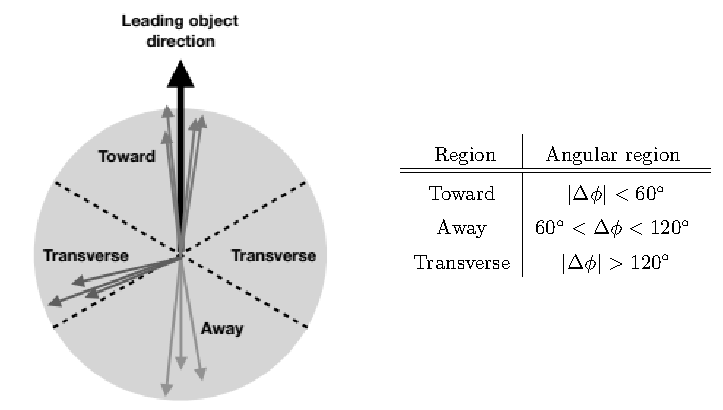
\includegraphics[width=0.8\textwidth]{{img/Regions.pdf}}
	\caption{This figure shows the four regions for the description of the UE on a event-by-event analysis. the angular values are shown in the table. The regions are defined starting from the leading object direction. The toward and away regions contain most of the contribution from the hard scattering (e.g. in a $t\overline{t}$ production event the two quark $t$ are located in these regions); while, the transverse region are the ones in between the twp other regions, these are the most important for the study of the UE.}
	\label{fig:Regions}
\end{figure}
%
\\
The regions classification is shown in \figRef{fig:Regions}, we have:
\begin{itemize}
	\item \textbf{Toward region}: the region that contains the leading object, this region contains the most of the particle produced by the hard interaction.
	\item \textbf{Away region}: this region contains the objects that recoil against the leading object, also this region contains mostly the particles produced by the hard interaction.
	\item \textbf{Transverse regions}: the two transverse regions are the most sensitive to UE.
\end{itemize}
The transverse regions are also separated in:
\begin{itemize}
	\item[--] \textbf{TransMAX}: This is the transverse region that contains the \textit{maximum} number of charged particles, or scalar $p_T$ sum of charged particles. This regions includes both MPI and hard-process contamination.
	\item[--] \textbf{TransMIN}: is the transverse region that contains the \textit{minimum} number of charged particles, or scalar-$p_T$ sum of charged particles. This region is the most  sensitive to MPI effects.
\end{itemize}

The leading object definition depend on the type of event under observation. 
The charged-particle with largest $p_T$ \cite{CMS-PAS-FSQ-15-007}, the dilepton system in Drell-Yan observation \cite{CMS:2012oqb, CMS:2017ngy} or $t\overline{t}$ events \cite{CMS:2018mdd} can all be used as leading object in the analyses for the UE event.
\\
So we are interest in studying the transMAX and transMIN region in particular the observable sensitive to UE in these regions are: the charged-particle density and the charged-particle scalar-$p_T$ sum density in the $\eta-\phi$ space

In an hadron-hadron collision with two jets productions it is observed that also the transverse regions activity increase with energy, as shown in \figRef{fig:UEpredictions_in_regions.png}, where the different color lines refer to different scales for the collision. Is observed that the away region ($60\leq |\Delta\phi|\leq 120$) at increasing energy for the collision become broader this is related to the increasing quantity of FSR.
\\
This increment in the transverse regions activity cannot be explained only by the increase of the FSR. To explain this rise one need to attribute activity in the transverse regions to MPI, extra scattering increasing with energy is related to the partons inside the hadrons that become denser packed when probed at higher energies. 

\begin{figure}[!ht]
	\centering
	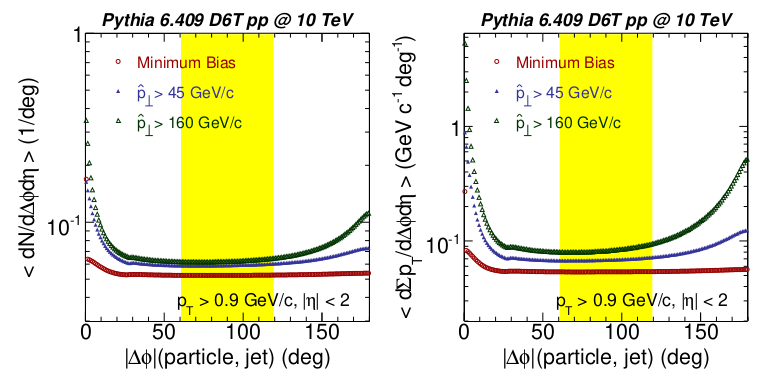
\includegraphics[width=0.8\textwidth]{{img/UEpredictions_in_regions.png}}
	\caption{A comparison between three different scales for the interaction. The multiplicity of charged particles (left) and the scalar-$p_T$ sum of charged particles (right) are simulated. The activity in the transverse regions increase due two effects: the FSR this is related to the broadening of the away region so some events from the shower end up in the transverse region (yellow band) but this alone can't explain the increment so is required the introduction of the MPI in the description. Figure from chapter 5 of \cite{Bechtel:2009zza}.}
	\label{fig:UEpredictions_in_regions.png}
\end{figure}

The evolution of these two quantities in transMAX region in function of the transverse-momentum of the leading object (measurement of the energy scale for the collision) is shown in more detail in \figRef{fig:CPtransmax_evolution_with_energy}. The two distribution show a rapid raise at low leading-object $p_T$ than a very low rise start.

\begin{figure}[!ht]
	\centering
	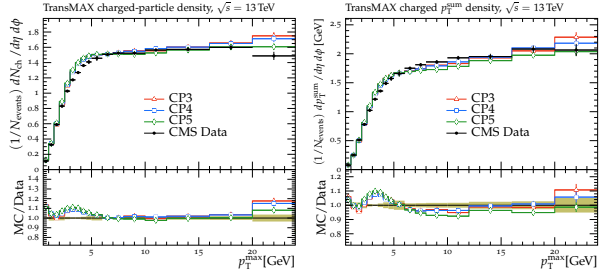
\includegraphics[width=0.8\textwidth]{{img/CPdistributions.png}}
	\caption{The evolution of the charged-particles density (left) and of the scalar-$p_T$ sum density of charged particles (right) as a function of the energy scale for the scattering (leading object $p_T$), the two distribution increase quite rapidly in the first bins than they saturate ($\approx 6-7\ \mathrm{GeV}$) the scalar-$p_T$ sum density increase a little bit more, for $p_T>$ but very slowly. The black dots are the experimental point and are compared to prediction with CMS \textsc{pythia} tunes: CP3, CP4 and CP5; they are described with more details in the next chapter. Figure from \cite{CPtunes}.}
	\label{fig:CPtransmax_evolution_with_energy}
\end{figure}

Now we want to look for the sensitivity of these observables to some \textsc{Pythia8} parameters. In figure \figRef{fig:CP5onlyPT0} is shown the effect of the MPI on booth the distributions shown before. The amount of the MPI is related to the value of $p_{T0}$: an high value of $p_{T0}$ is related to less MPI (blue line) and an higher value to a major contribution from the the MPI (red line).

\begin{figure}[!ht]
	\centering
	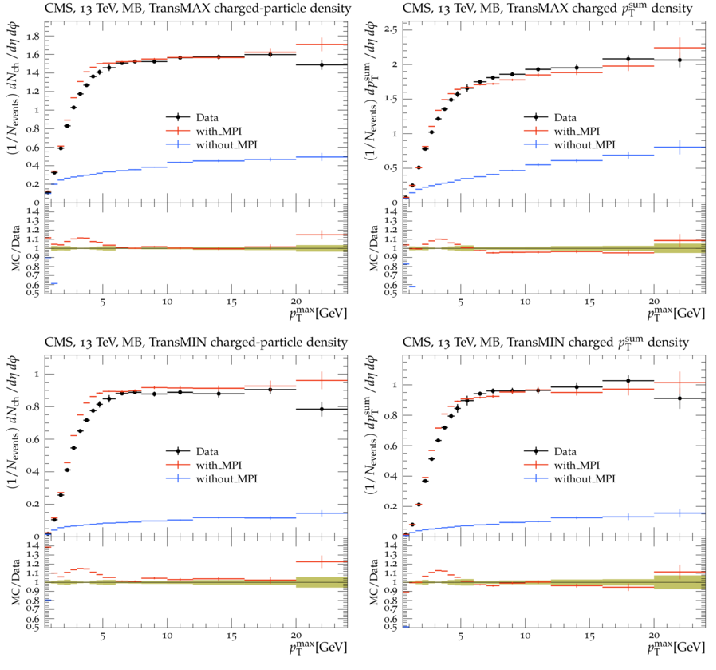
\includegraphics[width=0.8\textwidth]{{img/CP5_with_without_MPI.pdf}}
	\caption{This image shows the effect of the MPI in the transMAX and TransMin regions. The contribution of the parton shower alone can't explain the contributions of the underlying event in these two regions (blue line) the introduction of the contribution from the MPI is necessary (red line). The two simulations are compared to the data from \cite{CMS-PAS-FSQ-15-007}.}
	\label{fig:CP5onlyPT0}
\end{figure}

Another important observation that was also pointed out in the \chapRef{sec:BasicConcepts} is that the amount of activity in the two transverse regions is also dependent on the center-of-mass energy. This evolution is shown in \figRef{fig:CPECMdep} for two different energy. The amount of MPI increase with $\sqrt{s}$ that was expected from the evolution of the PDF with the energy of the collision: the hadrons become denser-packed when probed to higher energies.

\begin{figure}[!ht]
	\centering
	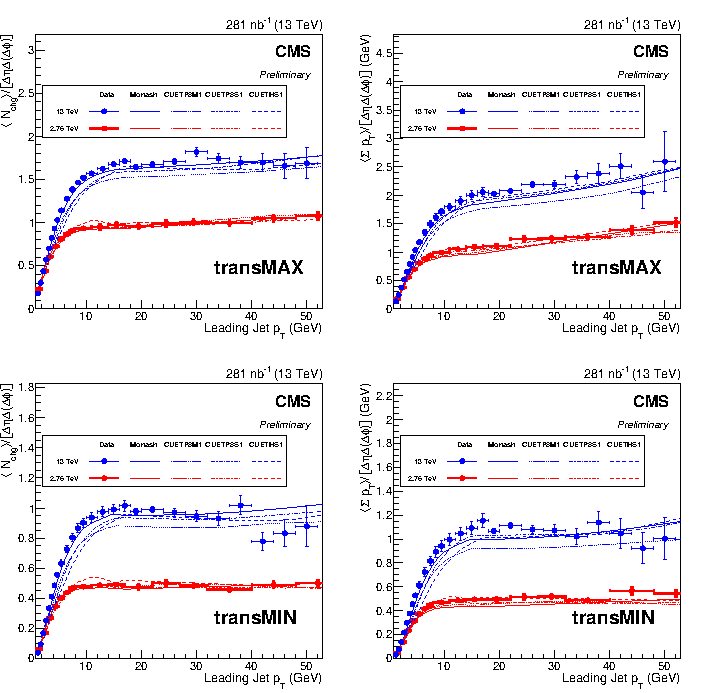
\includegraphics[width=0.85\textwidth]{{img/CPECMdep.pdf}}
	\caption{The charged particle density in the transMAX (upper left) and transMIN (lower left) regions and of the charged particle $p_T$-sum in the transMAX (upper right) and the transMIN (lower right) regions evolution as function of the center-of-mass energy is shown. The red ones are the data for $\sqrt{s}=2.76$ and the blue ones for $\sqrt{s}=13$ and these are compare to different CMS tunes. Figure from \cite{CMS-PAS-FSQ-15-007}}
	\label{fig:CPECMdep}
\end{figure}


}
	
\graphicspath{{TuneProcedureAndMCNNTUNES/}}
\chapter{Tune procedure and \textsc{mcnntunes}}
\label{chap:TuneprocedureCP5TuneandMCNNTUNES}

The study of the underlying event, or more in general of soft QCD processes require the use of Monte Carlo generators that often are based on phenomenological models with lots of free parameters. These free parameters must be tuned on experimental data in order to obtain meaningful results from the simulations. The procedure of estimate the best parameters values in order to best reproduce the observables under analysis is called \textit{tune}. 
\\
The tune procedure can be really computational expensive, in fact it requires to run the generator a very large amount of times, and usually these MC generators are really expansive in term of computational time required for just a single job.  
\\
To tune a certain number of parameters the number of jobs you have to run increase with this number of parameters. In fact, the parameters space dimension increase with the number of the sampling we want to perform and the granularity we want to achieve. So, in the past, different approaches have been developed and used to tune these MC generators. A brief description is reported for each approach in the following list:
\begin{enumerate}[label=\arabic*)]
	\item \textbf{Manual tunes}: this approach is based on an optimization of the parameters made by eye. This is absolutely not the best way to tune some parameters, usually it requires a very large time for even semi-reasonable results since the process require a very large number of iterations .   
	\item \textbf{Brute force tunes}: a better way would be to perform a very dense sampling in parameters space, run the generator with every configuration and then chose the configuration corresponding to the output that better describes the experimental data. This is very computational expensive and a scan in a $5$ parameters space with $10$ division each requires $10^5=100000$ Monte Carlo runs this with a rising number of parameters becomes really impractical, also using computers batch systems as an example CondorHT (\textsc{cern}).   
	\item \textbf{Parametrization-based tunes}: an even more better approach is to find a surrogate function to parameterize the response of the MC generator at different values of the parameters to tune, and try to study (minimize) this surrogate function instead of the real response of the generator. This is the right approach that is used in the high energy physics tune and that we are going to use in the follow for our tune.
\end{enumerate}
Let us discuss this last approach with more details in the next section.

\section{Parametrization-based approach}

The parametrization-based approach is the most used method. The current state-of-art in the tune procedure is to use a polynomial function to fit the response of the generator. Once the parametrization is performed the tuned parameters are given by the minimization of this parameterized response function. This approach based on the polynomial parametrization have been  implemented in the software \textsc{Professor} \cite{Buckley:2009bj}. 
\\
So the first step in the procedure is to fit the response of the generator using a surrogate function simpler to study than the real one (e.g. Professor instead of the arbitrary complex real function use a polynomial fitted to well describe the real function).
\begin{equation}
	h(p)\ \xrightarrow{\quad \text{parametrization}\quad }\ \overline{h}(p)\quad ,
\end{equation}
where the real function have been substituted by the surrogate one. 
\\
After that, a \textit{loss function} $\mathcal{L}(\overline{h}(p),h_{\text{data}})$ is defined between the surrogate function and the experimental data. A common choice for it is the $\chi^2$ function defined as:
\begin{equation}
	\mathcal{L}(\overline{h}(p),h_{\text{data}})\equiv \chi^2=\frac{(\overline{h}(p)-h_{\text{data}})^2}{\sigma^2}\quad.
\end{equation}
In the end to find the best parameters estimation, this loss function need to be minimized. The set of parameters $p_{\text{best}}$ that do this are the best evaluation that our generator can provide for the real values and we are going to call this set of best parameters: \textit{tune}.
\begin{equation}
	p_{\text{best}}=\arg\,\min_p\ \mathcal{L}(\overline{h}(p),h_{\text{data}})\quad.
\end{equation}
In our study instead of the common software \textsc{professor} based on the polynomial parameterization we use the machine learning approach implemented in \textsc{mcnntunes} software \cite{MCNNTUNESonGitHub}
using Feed Forward Neural Networks. \textsc{mcnntunes} is a software developed by S. Carazza, S. Aioli and M. Lazzarin presented in \cite{MCNNTUNESarticle} based on machine learning library TensorFlow \cite{tensorflow2015-whitepaper}. \textsc{mcnntunes} is writen in python and it uses neural networks (NNs) that are trained in order to learn the generator behavior to the parameters variations. This remove the polynomial constraint in the fit of the generator respond function in fact one of the main feature of the Neural Network is that they are universal function approximators.
\\
Let's make a brief introduction on machine learning and in particular on neural networks in order to understand why this choice.

\section{Machine Learning and Neural Networks}
  
Machine learning (ML) is a particular type of Artificial Intelligence it consists in systems that learn automatically by the data that are fed into it and not by the explicit programming of the algorithm. It is clear that ML requires the training of the algorithm in order to have a predictive output related to the problem under analysis. The training is the most important step in the ML approach in fact is this step that gives to the ML the ability to return a predictive output without it the output we get is not able to give us a meaningful result.
\\
A particular type of ML is Deep Learning that uses neural networks with more than one layer organized in a hierarchical structure to solve the problem. This is the type of ML we are interested in. But before we start with the explanation of the simple possible neural network that can be created in order to understand the basis in the logic of each unit that is going to compose the neural network. 


\subsection{Neural Networks - Perceptron}

The concept of the Neural Network (NN) was developed in 1958 by Frank Rosenblatt. He introduce the simpler example of NN: the perceptron \cite{Perceptron}. A representation of a percepton is shown in \figRef{fig:Perceptron} the input values are weighted and summed, an additional offset $b$ can be introduced, then the weighted-sum is passed to an activation function (step function). So, the output that the perceptron returns is:
\begin{equation}
	h(x)= \text{step}\bigg(\displaystyle\sum_j w^j\, x_j + b\bigg)
\end{equation}

\begin{figure}[!htb]
	\centering
	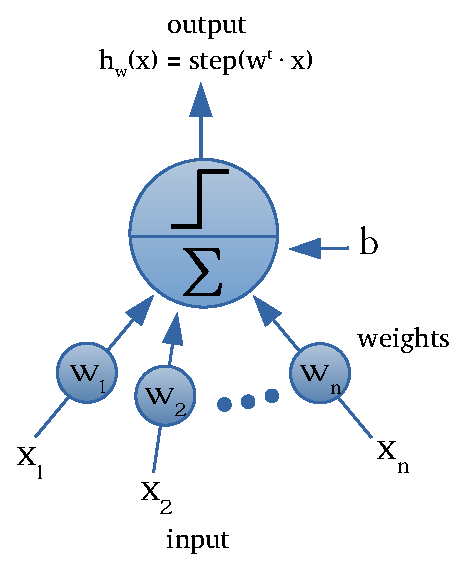
\includegraphics[scale=0.7]{{img/Perceptron2.pdf}}
	\caption{A schematic representation of a perceptron.}
	\label{fig:Perceptron}
\end{figure}

\noindent The revolutionary feature of the perceptron was the ability of learning by an adjustment of the weights. But a single perceptron is not enough this kind of logical units have lots of limitations. An example of limitation for the perceptron is shown in \figRef{fig:XORproblem} where the impossibility of implement a \textsc{xor} operation using a perceptron is shown with a graphical explanation. The perceptron is a linear classification algorithm and in the image is represented as a blue line that set a boundary for the acceptation of the hypothesis.

\begin{figure}[!htb]
	\centering
	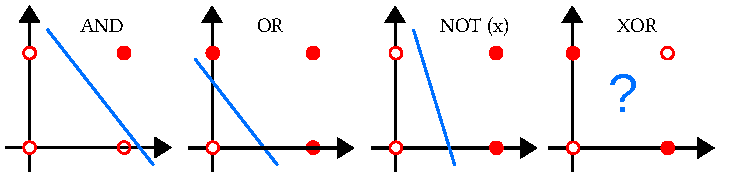
\includegraphics[width=14cm]{{img/XORproblem.pdf}}
	\caption{The figure shows one of the limitations of the perceptron. The \textsc{xor} operation is not possible with a linear cut.}
	\label{fig:XORproblem}
\end{figure}

The structure is very simple with a single unit but is not enough it have a lot of limitation so we have to introduce the concept of NN with more than one unit if we want eliminate these limitations and approximate every type of functions.

\subsection{Feed-Forward Neural Networks}

In a Neural Network different units called "neurons" are linked together. Different type of NNs exist and they are classified according to the various ways the neurons are linked each other. We are interested in \textit{fully-connected Feed-Forward NNs}, that are the ones used in \textsc{mcnntunes}. 
\\
In fully-connected NNs each neurons from a layer are connected to every neurons in the next layer. While, the Feed Forward attribute refers to the fact that the NN have not internal recursions (loops) between neurons but all the neurons from a layer are connected forward to the ones of the next layer.
\\
\figRef{fig:NNesample} shows a schematic view of a fully-connected feed-forward multi-layer NN the basic idea is that the neurons can get some value in input and return a value as output. The output of neuron is then sent to all the neurons in the next layer and weighted differently for each one. 
To be more specific: each unit $j$ in the hidden layer $(i)$ takes a vector of values $x^k$, that come from all the $k$ neurons of the previous layer, and an offset $\vartheta_j$ as input, compute the weighted sum $\sum_k w_{kj}x^k$ and apply the activation function $\phi$ to the result, common choices for this function are \textit{tanh} or \textit{sigmoid} functions. So, the total output of the $(i)$-th layer in the network is the function:
\begin{equation}
	f^{(i)}(x) = \displaystyle\sum_{j=1}^{N^{(i)}} \varphi \left( \displaystyle\sum_k w^{(i)}_{kj}x^k + \vartheta_j^{(i)} \right)\quad,
\end{equation}
where $N^{(i)}$ is the number of hidden units in the $(i)$-th layer. 
\\ 
One of the biggest feature of the NNs is that the they are universal function approximators \cite{HORNIK1991251, LESHNO1993861} the only request for this is that a sufficient number of hidden layers is available. This is the main reason why we want use a NN based approach instead of the polynomial one
\\

\begin{figure}[!htb]
	\centering
	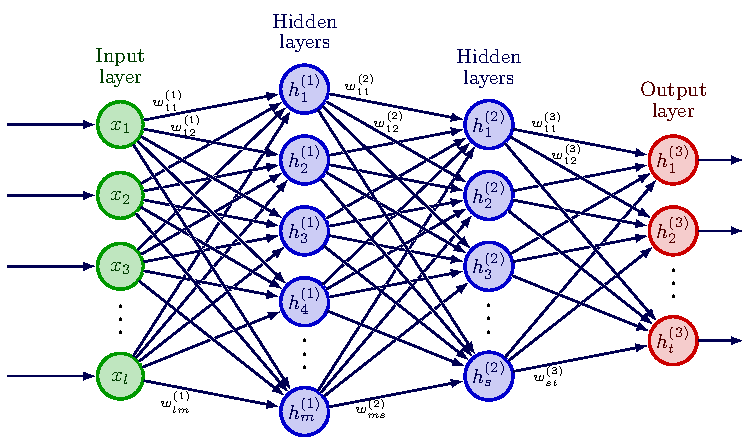
\includegraphics[width=0.95\textwidth]{{img/NN.pdf}}
	\caption{A fully-connected feed-forward neural network with more than one hidden layer, the green one is the input layer and takes the value in input and usually scale them in the range $[0,1]$ and then the data sequentially go trough the neurons in the hidden layers (blue) where all the steps described above are performed for each layer. At the end the results of the computation are collected by the output layer (red). }
	\label{fig:NNesample}
\end{figure}

\noindent As mentioned before the main feature of all the types of NNs is the ability to learn from data without being directly programmed.
But to to this and so get some predictive results from the NN a learning algorithm have to be defined.
\\
A common training algorithm for the NN is the \textit{back-propagation}. Where a set of Monte Carlo simulations is used to train the NN. The back-propagation procedure is based on the idea of change the weights, $w_{jk}$, and the offsets, $\vartheta_{j}$, in order to minimize a loss function usually defined as the mean squared error ($E$):
\begin{equation}
	E=\frac{1}{2}\displaystyle\sum_i(h_{i}(x^j,w_{jk})-d_i)^2\quad,
\end{equation}  
where the $h_{i}$ are the value in output from the NN and the $d_{i}$ the real value known from the Monte Carlo truth.
\\
In the back-propagation algorithm the weight and the coefficients are update using the \textit{steepest-descent minimization}:
\begin{equation}
	w_{jk}^{(i+1)}=w_{jk}^{(i)}-\lambda\left( \frac{\partial E}{\partial w_{jk}} \right)^{(i)}
	\quad; \ \qquad
	\vartheta_{j}^{(i+1)}=\vartheta_{j}^{(i)}-\lambda\left( \frac{\partial E}{\partial \vartheta_{j}} \right)^{(i)}
	\label{eq:learning_bp}
\end{equation}
where $\lambda$ is the learning rate and is a user-tunable free parameter and it controls how much change the weights each time the weights are update.
It is one of the main parameter in the neural networks a to small value for it can lead to a failure in the training procedure while a to large one can lead to unstable results. 
\\
The mini-batch are subset of our training set that contains the Monte Carlo simulations that are used to calculate the gradient. The size of the mini-batches used to train the NN is also a free parameters: smaller batches are faster to compute but the gradient direction is not the real one just an approximation; while bigger batch size give a good approximation of the direction of the steepest-descent but can be computational expensive. 
\\
The number of evaluation of the entire training set is called epochs and is tunable by the user.
\\
Note that the batch size and the number of epochs are related. A training set of 50 run with a batch size of 10 and a number of epochs of 1000 require 5000 iterations while if we use a batch size of 25 it require only 2000 iterations to run over all the training set.
\\
A schematic representation of the training process is displayed in \figRef{fig:training2} where the training set is subdivided in the mini-batches that one by one are fed to the NN. Then, the Monte Carlo truth and the output of the network are used to compute the loss function $E$, using this information the back-propagation, based on the gradient descend algorithm, updates the weights in the descent direction of the gradient calculated using the mini-batch. All the procedure is repeated with every mini-batch and for a user tunable number of epochs.

Note that the prediction capability of the Neural Network is dependent on the selection of all these user-tunable parameters that control the Neural Network architecture. All these parameters are usually referred as \textit{hyperparameters}. 

\begin{figure}[!htb]
	\centering
	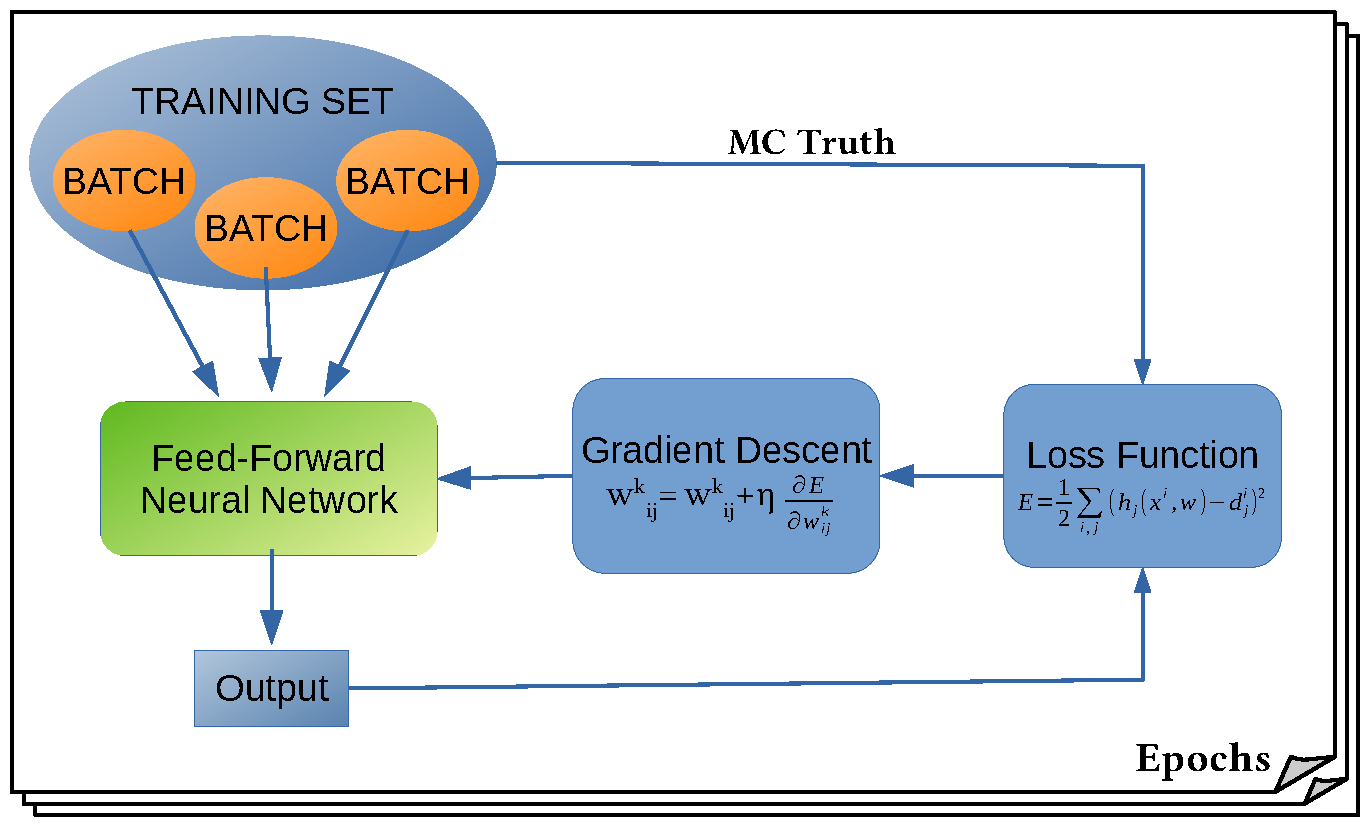
\includegraphics[width=14cm]{{img/Training2.pdf}}
	\caption{The training set used to train the NN is divided in mini-batch (the mini-batch size is a user tunable parameter) than one by one the baths are feed to the NN the output of the network together with the Monte Carlo truth are used to calculate the loss function. Then the weights and the offset are updated as described in \eqRef{eq:learning_bp} with the back-propagation algorithm. This is done with each mini-batch in the training set and for a number of epochs defined from the user. }
	\label{fig:training2}
\end{figure}


%%%%%%%\section{Previous Tune for the Underlying Event} OLD

In the next section \texttt{mcnntunes} is introduced and all its working modes are explained in detail. 

\section{MCNNTUNES}

\texttt{mcnntunes} \cite{MCNNTUNESarticle} is a Shower Monte Carlo generators tuning tool that implements a tune procedure based on the use of Feed Forward Neural Networks (FFNNs). The advantage of using FFNNs have been described above and is that they are universal function approximators at the simple cost of have a sufficient number of hidden units in the hidden layers. This feature allows us to remove the polynomial bias present in \texttt{professor} tool.
\\
\texttt{mcnntunes} offers two different main operation modes: \textit{PerBin Model} and \textit{Inverse Model}. The first one is based on approach similar to the one in \texttt{professor} but where the response of the generator is parameterized using these FFNNs, one for each bin; the later is a totally new approach where the NN (only one in this case) is trained to learn the inverse function of the generator response and then used to try to infers the parameters value starting the experimental values of the bins in the distributions used.
\\

\medskip

\subsection{Sampling Phase and Training Set Generation}

The two approach have the same starting point that is a sampling of the parameter space (e.g. for the UE analysis we use the parameters space shown in \tableRef{table:CP5variations}), than the generator is run with every sampled configuration. 
All these MC runs are going to build our dataset that is called \textit{training set}.
\\
A schematic explanation of how the sampling phase and the training set generation were performed in CMSSW environment (lxplus \textsc{cern}) is shown in \figRef{fig:worksampling}. 
In more detail the sampling start by mean of \textsc{mcnntunes} script called \textsc{mcnntemplate} with a sampling of the defined parameter space. The sampling generates  $N$ different configuration for the parameters to tune, this are then encapsulated in a runcard for \textsc{pythia} that contains all the necessary information to make \textsc{pythia} work properly (beams energies, type of event to simulate etc.). Then the \textsc{pythia} generator is run with every configuration generated and this is performed not locally but on a computers batch (e.g. the \textsc{cern} one CondorHT). The runcards we pass to Condor contain also the information on the analysis we want to performe and on how to fill the various histograms for the observables. Once the generators runs end the outputs are saved in the \textsc{yoda} format, that is a particular type of data file. The set of these \textsc{yoda} files, containing the information on the MC runs, composes our training set that then can be used for tuning procedure.

\begin{figure}[!htb]
	\centering
	\includegraphics[width=0.95\textwidth]{{img/Worksampling.pdf}}
	\caption{A schematic description of the main step from the sampling phase to the generation of the training set used for the tune procedure. These shows how the work was performed in CMSSW environment. The starting point and the final tune procedure are both controlled by \textsc{mcnntunes}. In the middle of these two phases the generation of the training set is required, this is performed running the generator many times.}
	\label{fig:worksampling}
\end{figure}

\medskip

\textsc{mcnntunes} offer also the possibility of change the value of the hyperparameters. The value that can be modified for the Neural Network. It is possible to chose the NN architecture: the number of hidden layer, the number of neurons for each layer and the activation function used. It is also possible to set the number of epochs, the batch size and the learning rate in order to have the best train for the architecture selected and other choice are possible. This is really important in order to get the best possible results for the tune.

\subsection{Per Bin Model}
\label{sec:PerBinModel}

PerBin Model is a parametrisation-based method. The main idea, as shown in \figRef{fig:PerBinModel_schematic} is to build a model (i.e. a neural network) for each bin in order to parameterize the generator output. Each NN takes the parameters values as input and returns the bin value as output.
\\
All these NNs are then trained feeding the MC runs from the training set and  using a gradient-based algorithm, as usual for feed forward neural networks, with mean squared errors as loss function.
\\
Once, the NN is trained, the last step is the tune in which one actually get the best parameters estimation.  This step define a surrogate loss function for the tuning problem. In fact, the parameterization step return a model $h^{(i)}(\mathbf{p})$ for each bin, $i$, where $\mathbf{p}$ is the vector of the parameters. 
\\
Then, this surrogate loss function defined as:
\begin{equation}
	\chi^2=\displaystyle\sum_{i=1}^N\frac{\left( h^{(i)}(\mathbf{p})-h_{exp}^{(i)}\right)^2}{\sigma_{(i)}^2}
\end{equation}
need to be minimized in order to evaluate the best estimation for the parameters. In \texttt{mcnntunes} this minimization is performed using the CMA-ES algorithm \cite{CMAES}.
\\
So the best estimation for the parameters is the configuration of parameters that minimize this $\chi^2$.  

\begin{figure}[!htb]
	\centering
	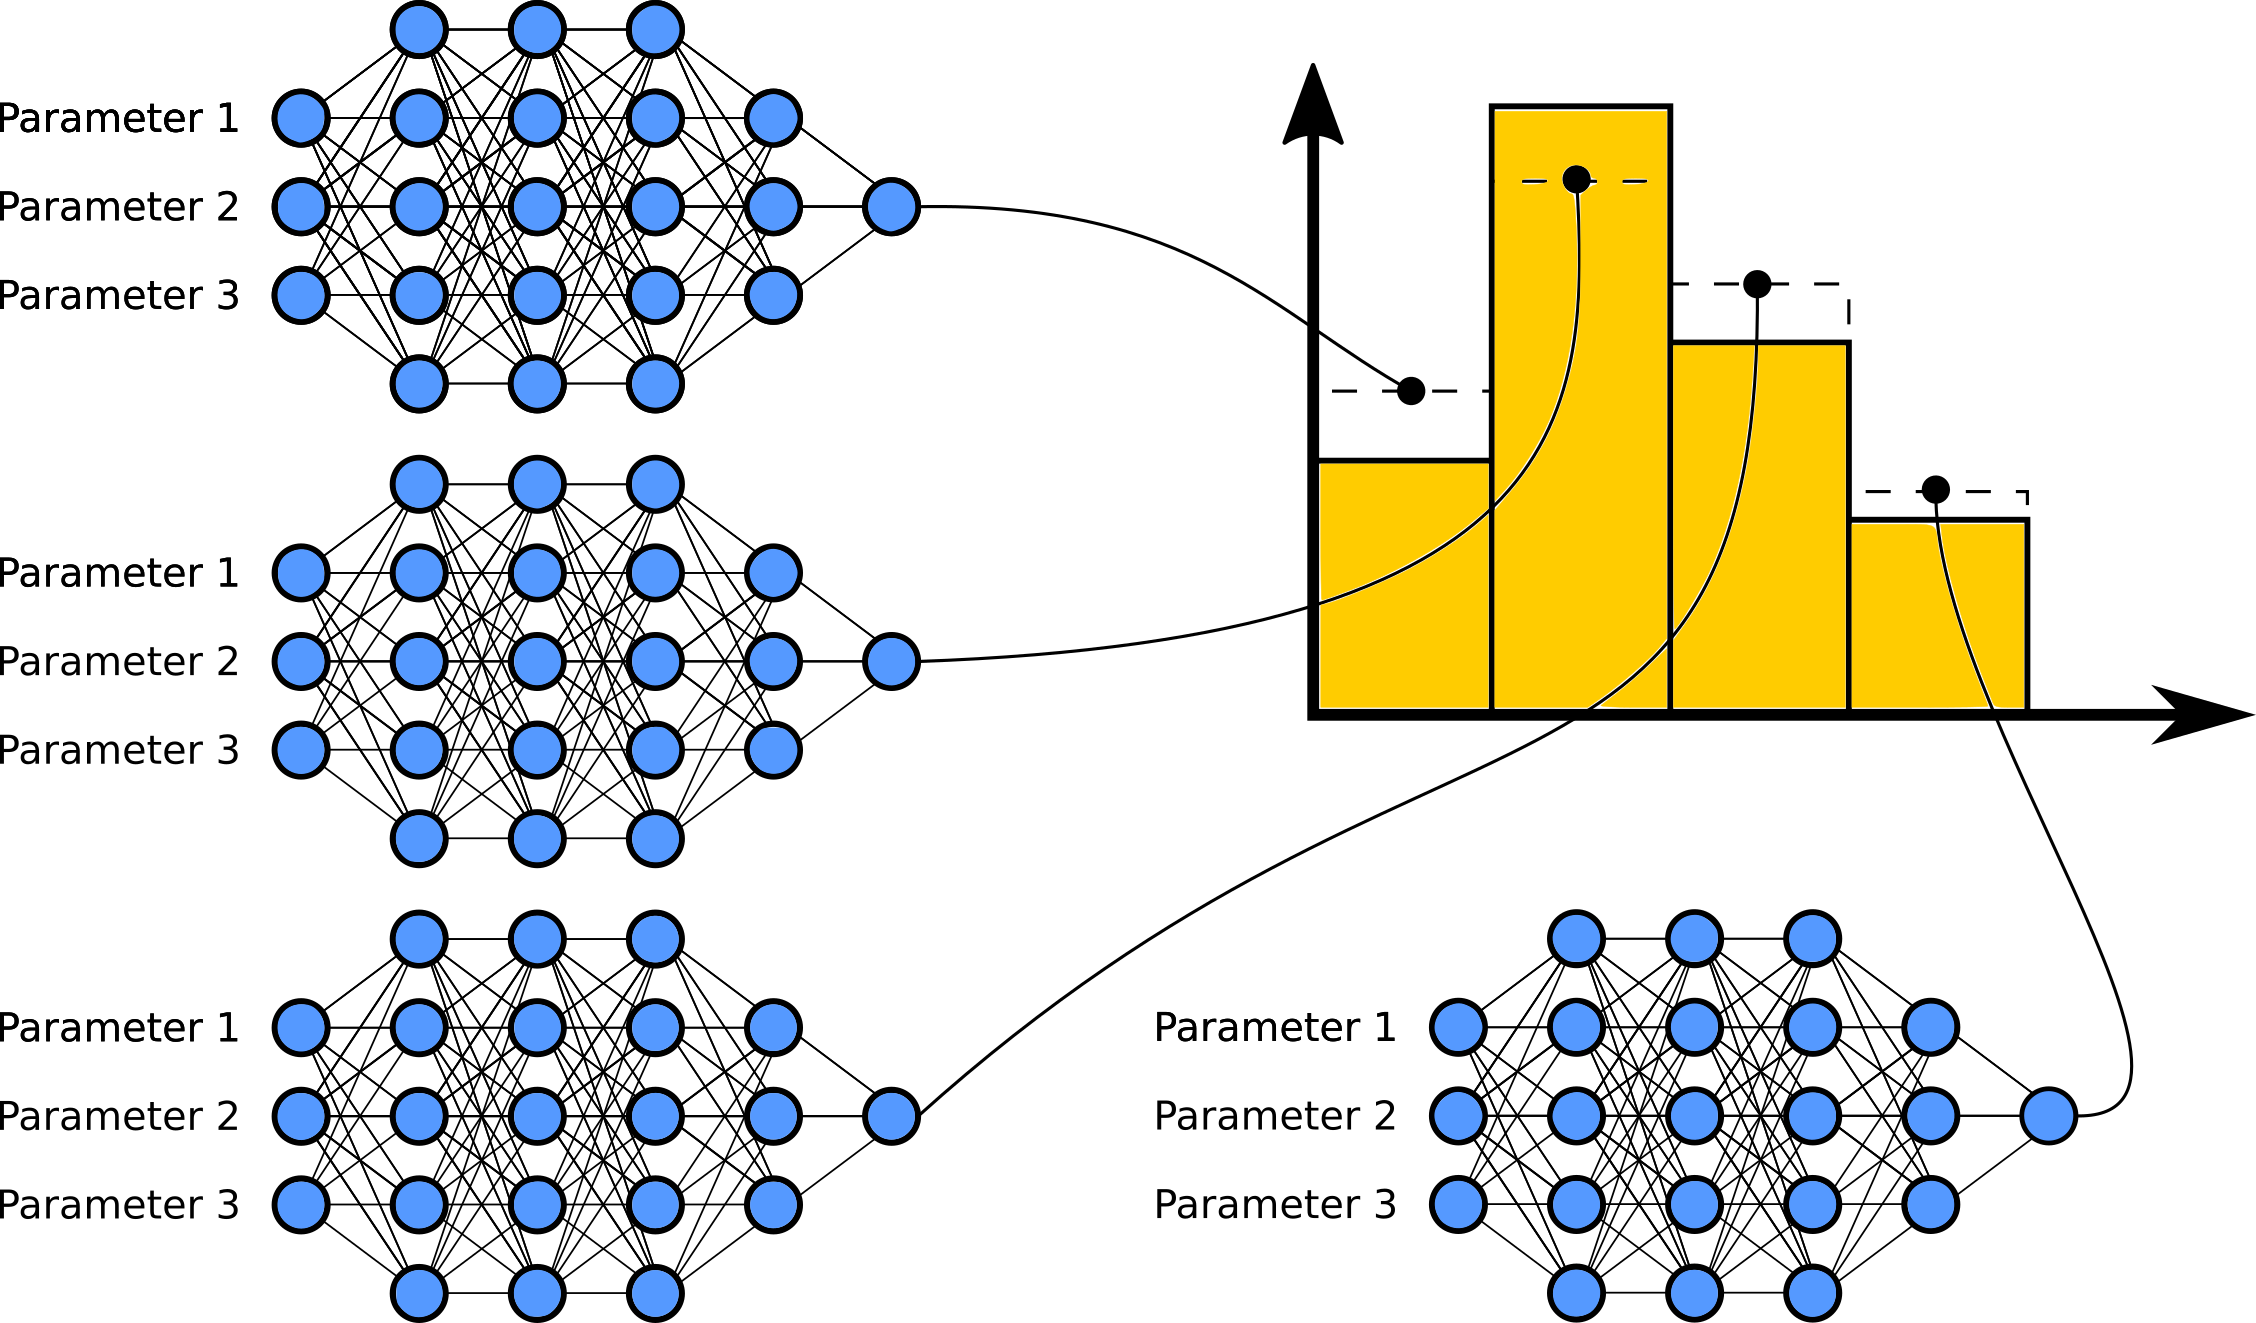
\includegraphics[width=0.8\textwidth]{{img/PerBinModel.png}}
	\caption{Figure from \cite{MCNNTUNESarticle}}
	\label{fig:PerBinModel_schematic}
\end{figure}

\subsubsection{Errors evaluation}

\textsc{mcnntunes} PerBin model as introduced in \cite{MCNNTUNESarticle} did not have a proper error evaluation. In fact it was using as error the final width of the distribution of sampled point in the CMA-ES algorithm. But, this was not working. Thanks to S. Carazza and with the help of M. Lazzarin we had the opportunity of handle the code and add a proper errors estimation.

Now, the errors evaluation for the PerBin Model is given by the definition of a confidence interval using the $\chi^2$ function.
In fact, as shown in section 9.6 and 9.7 of \cite{cowan}, for an estimators vector $\hat{h}(\mathbf{p})=(\hat{h}^{(1)}(\mathbf{p}),\hat{h}^{(2)}(\mathbf{p}),\dots,\hat{h}^{(n)}(\mathbf{p}))$ for the parameters $\mathbf{p}$ the probability distribution function and the likelihood (the $\chi^2$ in our case) in limit of a large sample\footnote{In other case this still a good approximation.} are Gaussian distributed. The probability distribution function for the estimators is than:
\begin{equation}
f(\hat{h}(\mathbf{p})|h(\mathbf{p})) = \frac{1}{(2\pi)^{n/2}|V|^{1/2}}\exp\left[ -\frac{1}{2}\left(\hat{h}(\mathbf{p}) - h(\mathbf{p})\right)^T V^{-1} \left(\hat{h}(\mathbf{p}) - h(\mathbf{p})\right) \right] \ ,
\end{equation}
where $T$ is the transpose vector and $V^{-1}$ is the inverse covariance matrix. 
Can be shown that also the likelihood is Gaussian as the probability distribution function. 
%So a changing in the parameter give a calculable variation in the $\chi^2$
So, we can define our confidence interval using the $\chi^2$ statistic as: 
\begin{equation}
	\frac{\chi^2(\text{c.i.})}{N_{dof}}= \frac{\chi^2_{min}}{N_{dof}}+\frac{Q_\gamma}{N_{dof}}
	\label{eq:chi2_variation}
\end{equation} 
The variation is dependent on the number of parameters and on the chosen confidence level ($1\sigma=0.683$ in our case) and a list of the values is reported in \tableRef{table:percentile}.

\begin{table}
	\centering
	\begin{tabular}{c | c c c c c}
		\multirow{ 2}{*}{percentile} & \multicolumn{5}{c}{$Q_\gamma$}\\\cline{2-6}
		& $n=1$ & $n=2$ & $n=3$ & $n=4$ & $n=5$ \\\hline\hline
		$0.683$& $ 1.00 $ & $ 2.30 $ & $ 3.53 $ & $ 4.72 $ & $ 5.89 $ \\
		$0.90$ &  $ 2.71 $ & $ 4.61 $ & $ 6.25 $ & $ 7.82 $ & $ 9.24 $ \\
		$0.95$ & $ 3.84 $ & $ 5.99 $ & $ 7.82 $ & $ 9.49 $ & $ 11.1 $ \\
		$0.99$ & $ 6.63 $ & $ 9.21 $ & $ 11.3 $ & $ 13.3 $ & $ 15.1 $ \\
	\end{tabular}
	\caption{The table report the values of the quantile $Q_\gamma$ for different confidence level $0.683$ is the row corresponding to the $1\sigma$ definition and is the one of our interest.}
	\label{table:percentile}
\end{table}

\noindent Then, the error is defined as the value of the parameters that give a deviation from the minimum value of the $\chi^2/N_{dof}$ equal to the $Q_\gamma/N_{dof}$ value for a confidence level of $0.683$, as defined in \eqRef{eq:chi2_variation}.
\\
An example for the evaluation in \texttt{mcnntunes} is shown in \figRef{fig:exampleChi2Variation} where the green line is the deviation from the minimum value of the $\chi^2$ defined in \eqRef{eq:chi2_variation} and the errors are given by the points where the $\chi^2/DoF$ reach these value. Therefore, the intersections between green and blue line that is the $\chi^2/N_{dof}$ for the different values of the parameter.

\begin{figure}[!htb]
	\centering
	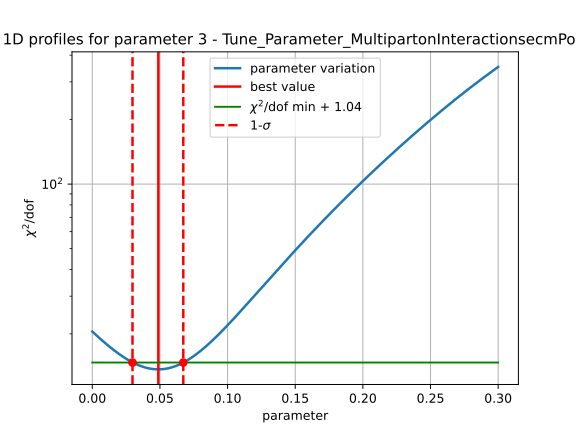
\includegraphics[width=0.6\textwidth]{{img/exampleChi2Variation.png}}
	\caption{This figure shows the error evaluation in \texttt{mcnntunes} for the \texttt{MultipartonInteractions:ecmPow} \texttt{Pythia8} parameter. The blue line is the value of the $\chi2/N_{dof}$ evaluated for different parameter values. The best estimation is indicated by the vertical red line, while the green line is the quantity in \eqRef{eq:chi2_variation}. The error is evaluated from the intersection of blue and green lines.
	}
	\label{fig:exampleChi2Variation}
\end{figure}

\subsection{Negative aspects}

One of the negative aspect is that this model is more computational expensive than the below discussed Inverse model. This is due to the large number of NNs built and trained from this model. 
The high cost in term of time required to get the model work do not give the possibility for a scan in the hyperparameters space in order to obtain the best configuration for the NN architecture. 
\\
This can impose some limitation on the model performance that cannot get its maximum  performance.

\subsection{Inverse Model}

The Inverse Model is the most innovative tuning procedure introduced by \texttt{mcnntunes}. This model contrarily to the PerBin Model takes the histograms bins as input and returns parameters values as output. For the Inverse Model the NN used is only one as shown schematically in \figRef{fig:InverseModel_schematic}. What the Inverse Model try to do is to learn the inverted model of the generator. So starting from the observed values the model try to reproduce the parameters values necessary to get the histograms we use as input.

The model is build and then trained with the training set introduced before. Once the model is trained feeding the experimental data to the NN this can try to infer the values of the parameters required to get the output. 

\begin{figure}[!htb]
	\centering
	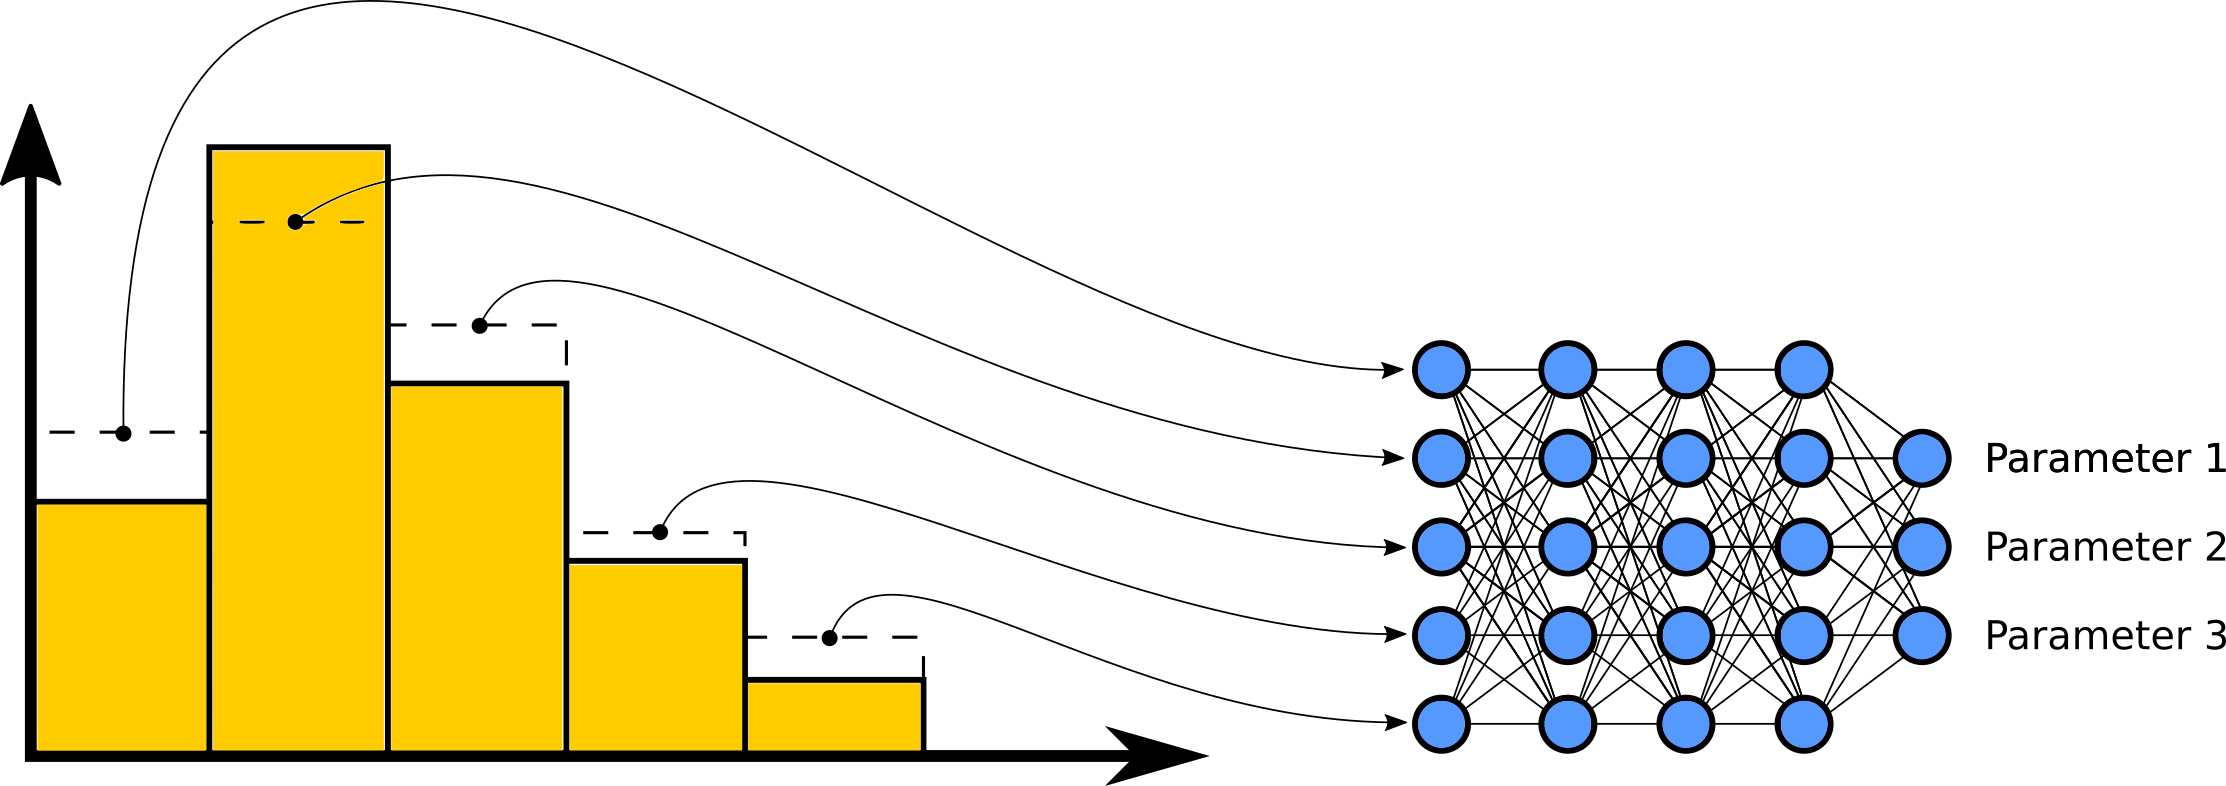
\includegraphics[width=0.8\textwidth]{{img/InverseModel.png}}
	\caption{Figure from \cite{MCNNTUNESarticle}}
	\label{fig:InverseModel_schematic}
\end{figure}

\subsubsection{Errors evaluation}

The errors are evaluated in a different way respect to PerBin Model in fact in the Inverse Model there is not a minimization step, and the error is evaluated by a re-sampling of the experimental data using a \textit{multivariate Gaussian Distribution}, as in \eqRef{eq:gaussianDristribution} with a diagonal covariance matrix that have experimental uncertainties on the main diagonal.
\begin{equation}
	f(x_i; h^{(i)}_{\text{exp}}, \sigma^{(i)}_{\text{exp}})\,=\,\mathcal{N}\cdot\exp\left[ 
	-\frac{1}{2}
	\displaystyle\sum_{j=1}^{N_{bins}}
	\frac{\left( 
	x_i - h^{(i)}_{\text{exp}} 
	\right)^2}{{\sigma^{(i)}_{\text{exp}}}^2} 
	\right]
	\label{eq:gaussianDristribution}
\end{equation}
So, a set of histograms is generated, then this is fed to the NN and a distribution of predictions is generated. An example is shown in \figRef{fig:InverseModel_predictionsSpread}, from this distribution one can compute the error by evaluating the standard deviation.

\begin{figure}[!htb]
	\centering
	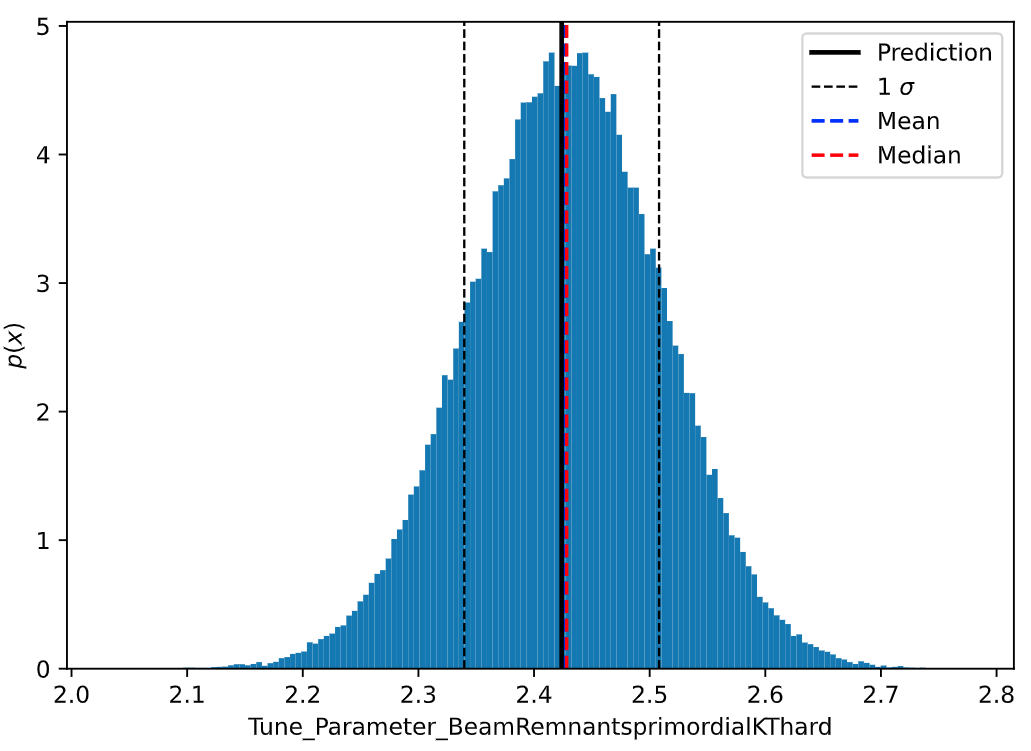
\includegraphics[width=0.6\textwidth]{{img/InverseModel_predictionsSpread.png}}
	\caption{Predictions spread for the inverse model after that a Gaussian resample is performed}
	\label{fig:InverseModel_predictionsSpread}
\end{figure}

Note that this is a new method for the tune. As we are going to see this method requires more attentions than the PerBin Model to get it working correctly in the case of an high number of parameters to tune.

Respect to the PerBin Model this method is faster. The NN trained is only one and is not needed a minimization so a scan in the hyperparameters can be performed in order to search for the best architecture. 

 
\subsubsection{Hyperparameters}

A really important step in the Inverse model is the \textit{hyperparameter optimization} it is required to get the method working. 

The procedure consist in build a \textit{validation set } containing some Monte Carlo simulations as the training set (e.g. $10\%$ of the simulations in the training set) and retrain the model with different choices for the NN architecture. Than a closure test is performed in order to estimate the performance of the NN and then the best model is retrained and the experimental data are fed to it in order to get the best estimation for the parameters to tune. This procedure is schematically summarized in \figRef{fig:HyperParams}.
\\
The hyperparameters scan is performed using the python package \texttt{hyperopt}.


\begin{figure}[!htb]
	\centering
	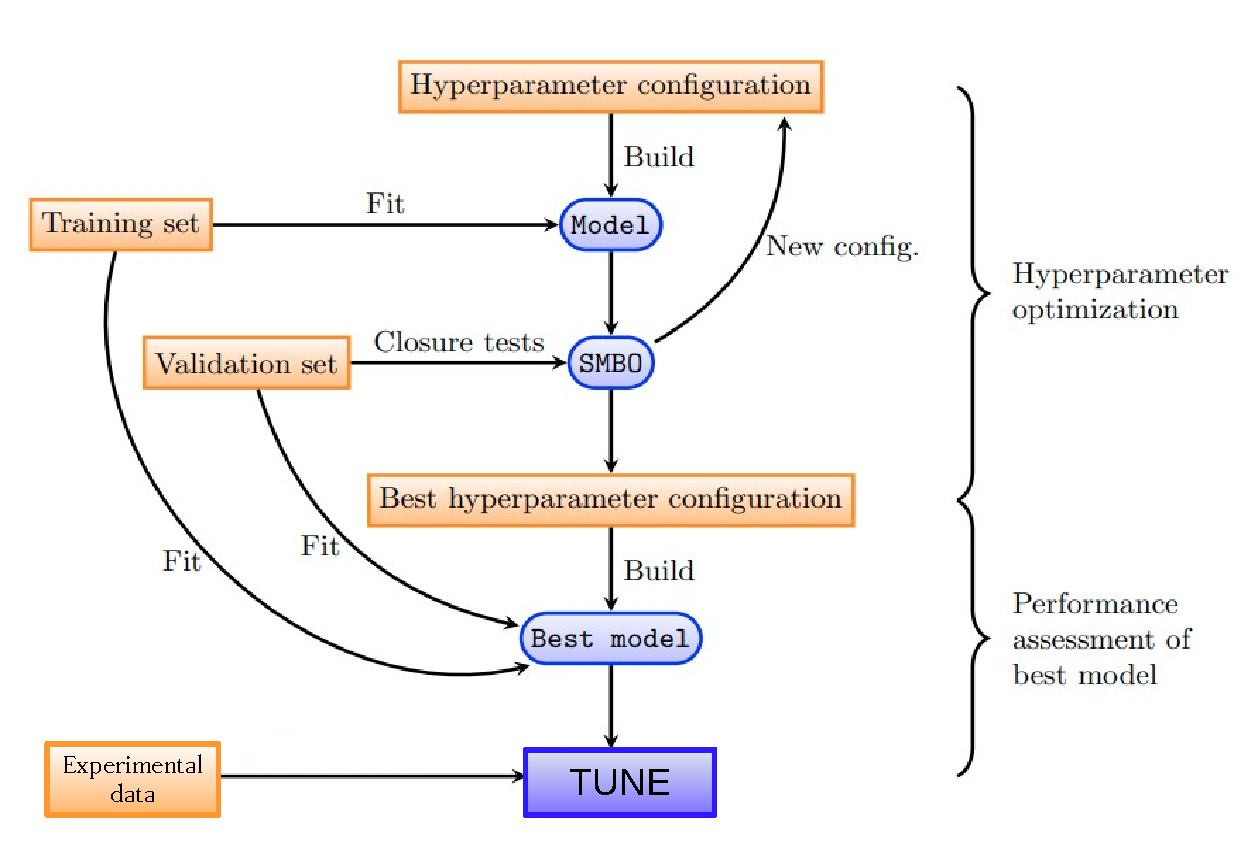
\includegraphics[width=0.9\textwidth]{{img/workflow.pdf}}
	\caption{The hyperparameter optimization procedure is schematically shown here. The model is trained using a training set than performing a closure test a scan on the hyperparameter is done. Once the best configuration is found the best model is retrained using both the runs in the training set and the runs in the validation set. Then the experimental data are fed the network and the best parameters are estimated. Figure from \cite{MCNNTUNESarticle}}.
	\label{fig:HyperParams}
\end{figure} 

\subsubsection{Problems}

As we are going to see the main problem for the Inverse model is the stability in the results. The operation that this model is trying to do is very hard, learn the inverse response of the generator is not an easy task. This difficulties in some case leads to a bad prediction. 
\\
As we are going to see in the chapter on our tune the inverse model requires some more attention than the PerBin model to get it work properly and in some case when the number of parameters became large and maybe the correlation between the parameters are important this model fails. 
\\
But if more care are given to this model this can become a very powerful method for future tunes.


\subsection{Weightrules in MCNNTUNES}

\textsc{mcnntunes} as \textsc{professor} implement the possibility of change the weight of the singles bins in the distributions. This is a really useful feature. As we will discuss later we use these weightrules to get a results more similar to CP5 in our tune. Increasing the weight of a bin this bin became more important in the overall $\chi^2$ evaluation and it is better described by the simulations. An example is shown in \figRef{fig:CMS_weightrules} where the application of the weightrules takes us to a better description of the experimental data.

\begin{figure}[!htb]
\centering
\noindent
	\includegraphics[width=0.85\textwidth]{{img/CMS2015_weightrules.jpg}}
	\caption{An example of weightrules application. Here the black point are the experimental data from the CMS analysis at $\sqrt{s}=13\ \mathrm{TeV}$ \cite{CMS:2015zrm} while the colored lines are the simulations, the vertical lines on MC points indicate the statistical uncertainties. It is easy to see that the distribution in the right panel is not well described from the tune, but thanks to the weightrules we can give to this distribution a greater importance in the tune and describes it better as shown in the left panel. This is better explained in the next chapter.}
	\label{fig:CMS_weightrules}
\end{figure}   


}	
	
\graphicspath{{OurTune/}}
\chapter{Our Tune for the Underlying Event}
\label{chap:OurTunefortheUnderlyingEvent}

This section focus on our work in order to reproduce a similar tune to CP5 one for the underlying event and minimum bias obseravbles. This is done to test the ability of \textsc{mcnntunes} of being one valid tool for the tuning of Monte Carlo generator with real data. 
\\
In order to validate \textsc{mcnntunes} as a good tool for the tuning we decide to firstly performer a simpler tune with only two free parameters and then try to reproduce CP5 \cite{CPtunes} with all the five parameters variation.


\section{Introduction}

We have performed a different tune for the underlying event and minimum bias observables using the same distributions, listed in \chapRef{sec:Thedistributionsused} and used in CP5 tune, so we expect to get a similar result from the tune using  \textsc{mcnntunes}.
\\
Just a quick reminder for the \textsc{pythia8} settings used in CP5 and in our tune:
\begin{itemize}
	\item The PDF set used is \textsc{nnpdf}3.1 calculated to the NNLO \cite{NNPDF:2017mvq}; 
	\item an $\alpha_s$ value equal for all the processes set to $0.118$ and running with a NLO evolution.
	\item The ISR is also ordered according to rapidity.
\end{itemize}
In the tuning procedure we employed both the \textsc{mcnntunes} operation modes described in the previous chapter: PerBin and Inverse models.

\section{First test: only two parameters variation}

The first simplified test we perform is the tuning varying of only two parameters. The parameter chosen are the \texttt{MultipartonInteractions:pT0Ref} and 
\\ 
\texttt{MultipartonInteractions:ecmPow}. These two parameters have been introduced in \secRef{sec:BasicConcepts}.
\\
The aim of this simplified test is to check the correct operation of \textsc{mcnntunes} in fact in a restricted parameters space it is simpler to learn the generator behavior and predict the corrects best values for the parameters. 
\\
\tableRef{table:variation_2params} shows the parameters space used in this first case. The other parameters are set to the CP5 values (also these are reported in the table as a reminder).

\begin{table}[!htb]
\centering
\begin{tabular}{l | c }
Parameter Name & Value \\ 
\hline \hline
\\[-0.85em]
	\texttt{MultipartonInteractions:pT0Ref} [$\mathrm{GeV}$] & $[1.0 - 3.0]$\\
	\texttt{MultipartonInteractions:ecmPow} & $[0.0 - 0.3]$\\
	\texttt{MultipartonInteractions:coreRadius} & $0.7634$\\
	\texttt{MultipartonInteractions:coreFraction} & $0.63$\\
	\texttt{ColorReconnection:range} & $5.176$
\end{tabular}
\caption{Parameters space for the two parameters test. The other parameters are set to the CP5 default values.}
\label{table:variation_2params}
\end{table}

\noindent Note: during this first part we don't use the two distributions related to the single diffractive and non single diffractive event selection for a bug on the routine of the analyses that have been fixed up before the real tune.  
\\
Let now discuss the results obtained for the test with the two models.

\subsection{Per Bin Model results}

The result we obtain for the PerBin model are reported in \tableRef{table:resultPerBin_2param}. The PerBin model estimation of the best parameters is performed by a loss function minimization. The output of the minimizer is reported in \figRef{fig:resultPerBin_2param}, the loss function ($\chi^2/\mathrm{dof}$) is the orange one, while the best parameter is marked by a solid red line.


\begin{figure}[!htb]
	\centering
	\noindent
	\begin{subfigure}{.45\textwidth}
		\centering
		\includegraphics[width=\textwidth]{{img/Plots_2params_Finale/chi2_0.jpg}}
	\end{subfigure}%
	\begin{subfigure}{.45\textwidth}
		\centering
		\includegraphics[width=\textwidth]{{img/Plots_2params_Finale/chi2_1.jpg}}
	\end{subfigure}
	\caption{The figure shows the output of the minimizer for each parameter. The right one refers to the \texttt{MPI:ecmPow} while the left one to the \texttt{MPI:pT0Ref}. The orange line is the $\chi^2/DoF$ as a function of the parameter values, the solid red line indicated the best estimation for the parameters.}
	\label{fig:resultPerBin_2param}
\end{figure}

\noindent The estimated parameters for the tune are also reported in \tableRef{table:resultPerBin_2param} with a comparison on CP5 boundary for each parameter. To be notice that the errors on the parameter estimated with PerBin model are not reported here because a correct error implementation, as the one described in \secRef{sec:PerBinModel}, was not yet implemented in the software at the moment of this test, but here we can see an example of the old error estimation. The old errors estimation process was not working in fact the errors lines (dashed red lines) are overlapped to the line of the parameter estimation in both the figures. The predicted errors were 3 or 4 orders of magnitude smaller then the parameter values. 
\\
But as we expected the results we get are similar to the ones obtained from the CP5 tune. The distributions obtained from the simulation using this parameters are shown below (\secRef{subsec:Overall2PARAMS}) together with results from Inverse model and CP5.

\begin{table}[!htb]
\centering
	\begin{tabular}{l | c | c}
		Parameter & Value & CP5 (down \& up) \\ \hline\hline
		\\[-0.85em]		
		\texttt{MultipartonInteractions:pT0Ref} & $ 1.46064$ & $1.41-1.46$\\
		\texttt{MultipartonInteractions:ecmPow} & $ 0.04771$ & $0.03$\\
	\end{tabular}
	\caption{Results for the PerBin model in two parameter variation test. The error evaluation was not correctly implemented yet and so the PerBin errors omitted in this table. The upper and lower limit for CP5 are also reported here for a direct comparison between the two tunes.}
	\label{table:resultPerBin_2param}
\end{table}

\medskip

An important observation is that our model is more sensible to some parameter respect to others.
\\
As an example, in \figRef{fig:param_vs_distributions} it is clear that our model is more sensible to the parameter \texttt{MultipartonInteractions:pT0Ref} (top) respect to 
\\
\texttt{MultipartonInteractions:ecmPow} (bottom). This is reflected in the output of the minimizer a greater sensibility gives a better defined minimum and vice versa. The top two panels show what happen when the distribution are very sensitive to the variation of the parameter as we can see on the left side the variation of the \texttt{pT0Ref} parameter leads to very different scenarios. This is reflected by the minimizer out in a well defined minimum and a smaller error on the parameter determination. A different scenario is displayed on the bottom panels of \figRef{fig:param_vs_distributions} where the distribution is less sensitive to the variation of the parameter \texttt{ecmPow} and so the minimum is less defined and so we are going to have a larger error on the estimation.

 
\begin{figure}[!htb]
\centering
\noindent
	\begin{subfigure}{.4\textwidth}
		\centering
		\includegraphics[width=\textwidth]{{img/Plots_2params_Finale/chi2_1.jpg}}
	\end{subfigure}%
	\begin{subfigure}{.07\textwidth}
		\centering
		\hspace{-4pt}\includegraphics[width=\textwidth]{{img/blueRightarrow.pdf}}
	\end{subfigure}%
	\begin{subfigure}{.4\textwidth}
		\centering
		\includegraphics[width=\textwidth]{{img/Plots_pTzero/CMS_2015_PAS_FSQ_15_007/d01-x01-y01.pdf}}
	\end{subfigure}\\
\centering
	\begin{subfigure}{.4\textwidth}
		\centering
		\includegraphics[width=\textwidth]{{img/Plots_2params_Finale/chi2_0.jpg}}
	\end{subfigure}%
	\begin{subfigure}{.07\textwidth}
		\centering
		\hspace{-4pt}\includegraphics[width=\textwidth]{{img/blueRightarrow.pdf}}
	\end{subfigure}%
	\begin{subfigure}{.4\textwidth}
		\centering
		\includegraphics[width=\textwidth]{{img/Plots_ecmPow/CMS_2015_PAS_FSQ_15_007/d01-x01-y01.pdf}}
	\end{subfigure}
	\caption{the sensibility of the tuned distributions respect to the variation of the parameters in related to the output of the minimizer. The top panels are related to \texttt{pT0Ref} while the bottom ones to \texttt{ecmPow}. The different colored lines in the 2 distributions (on the right) are the simulations with different values for the parameter. The black point are the data. }
	\label{fig:param_vs_distributions}
\end{figure}

\clearpage
\subsection{Inverse Model results}

The other operation mode offered by \textsc{mcnntunes} is the Inverse model. 
The results we get from the first test of the Inverse model are described here while the overall distribution are reported in next section together the ones from the PerBin Model. 
\\
As mentioned before to make this model work properly one have to perform a hyperparameters optimization. our hyperparameter optimization was a scan of the architecture parameters shown in \tableRef{table:hyperpar_MinBias_2par} the number of trials (combinations of these parameters) was $1000$. in this case the best model we found is the one reported in \tableRef{table:hyperpar_2parTEST}.
\begin{table}[!htb]
	\centering
	\begin{tabular}{| l | c |}
	\hline
	Hyperparameter & Variation Range\\[2pt]\hline
	Number of hidden layer & 2-5 \\[2pt]
	Units per layer & 2-20 \\[2pt]
	Activation function & tanh, relu, sigmoid \\[2pt]
	Optimizer & {\small sgd, rmsprop, adagrad, adadelta, adam, adamax, nadam}\\[2pt]
	Epochs & 250-15000 in discrete steps\\[2pt]
	Batch size & 64-5000 in discrete steps\\[2pt] \hline
	Number of trials & 1000\\[2pt]\hline
	\end{tabular}
	\caption{Hyperparameter space scanned for the optimization of the NN architecture.}
	\label{table:hyperpar_MinBias_2par}
\end{table}


\begin{table}[!htb]
	\centering
	\begin{tabular}{ l | c }
	Hyperparameter & Value\\[2pt]\hline\hline
	Number of hidden layer & 4 \\[2pt]
	Units layers & [2,\,14,\,9,\,18] \\[2pt]
	Activation function & tanh \\[2pt]
	Optimizer & nadam\\[2pt]
	Epochs & 1000\\[2pt]
	Batch size & 500\\[2pt]
	\end{tabular}
	\caption{Best hyperparameters model found for the test with 2 parameters variation.}
	\label{table:hyperpar_2parTEST}
\end{table}

\noindent Once the best model is trained the output we get from this model is the distribution of predictions obtained by the resampling phase of the experimental data then fed to the network. The prediction spread for the two parameters test is shown in \figRef{fig:ResultInverse_2params} these are obtained from the re-sampling phase using the multivariate Gaussian distribution described in \eqRef{eq:gaussianDristribution}. 

\begin{figure}[!htb]
	\centering
	\includegraphics[width=0.9\textwidth]{{img/Plots_2params_Finale/2params_prediction_spread.jpg}}
	\caption{The spread of predictions we get as output from the Inverse Model. the right one refers to the \texttt{ecmPow} parameter and the left one to \texttt{pT0Ref}. The parameters predicted are marked by the solid black line while the error is evaluated using the standard deviation indicated by the dashed black lines.}
	\label{fig:ResultInverse_2params}
\end{figure}

\noindent The estimated parameter are marked by the solid black line, while the dotted black lines are the error on the parameter.
The value we get from the tune are also reported in \tableRef{table:ResultInverse_2params} together with the CP5 values.
In this case the error estimation is correctly implemented and a direct comparison between the value is possible. Looking at the values reported in the table it is clear that the two tune are compatible. 



\begin{table}[!htb]
\centering
	\begin{tabular}{l | c | c}
		Parameter & Value & CP5 (down \& up)\\ \hline\hline
		\\[-0.85em]		
		\texttt{MultipartonInteractions:pT0Ref} & $ 1.43 \pm 0.14 $ & $1.41 - 1.46$ \\[2pt]
		\texttt{MultipartonInteractions:ecmPow} & $ 0.0298 \pm 0.0095 $ & $0.03$\\[2pt]
	\end{tabular}
	\caption{Results for the Inverse model in two parameter variation test. The upper and lower limit for CP5 are also reported here for a direct comparison between the two tunes. The two predicted parameters are compatible to the one in CP5.}
	\label{table:ResultInverse_2params}
\end{table}


\clearpage
\subsection{Overall results}
\label{subsec:Overall2PARAMS}

In this section we are going to show some overall results for the first test with only two free parameters. We are not going to show all the graphs here we list them all in the appendix \refApp{appendix:test}.
\\
From the graphs in \figRef{fig:result_2params_1} is clear that \textsc{mcnntunes} gives some good result for the test. 
\begin{figure}[!htb]
	\centering
	\noindent
	\begin{subfigure}{0.45\textwidth}
		\centering
		\includegraphics[width=\textwidth]{{img/Plots_2params_Finale/CMS_2015_PAS_FSQ_15_007/d01-x01-y01.pdf}}
	\end{subfigure}%
	\begin{subfigure}{0.45\textwidth}
		\centering
		\includegraphics[width=\textwidth]{{img/Plots_2params_Finale/CMS_2015_PAS_FSQ_15_007/d02-x01-y01.pdf}}
	\end{subfigure}\\
	\begin{subfigure}{0.45\textwidth}
		\centering
		\includegraphics[width=\textwidth]{{img/Plots_2params_Finale/CMS_2015_PAS_FSQ_15_007/d05-x01-y01.pdf}}
	\end{subfigure}%
	\begin{subfigure}{0.45\textwidth}
		\centering
		\includegraphics[width=\textwidth]{{img/Plots_2params_Finale/CMS_2015_PAS_FSQ_15_007/d06-x01-y01.pdf}}
	\end{subfigure}
	\caption{Results for the two parameters variation test. Here are reported the  distributions from the $\sqrt{s}=13\ \mathrm{TeV}$ CMS analysis \cite{CMS-PAS-FSQ-15-007} that show the transMAX charged particle density (upper left) and the charged $p_T$-sum density (upper right); the transMIN charged particle density (lower left) and the charged $p_T$-sum density (lower right) as a function of the transverse momentum of the leading charged particle. The black points are the experimental data and the black vertical lines the experimental uncertainties. The data are compared to the MC prediction from the result we get using PerBin Model (green line), Inverse Model (blue line) and the existing tune CP5 (red line). The data are well described by all the tunes. Our tune describe very well the low-$p_T$ region ($p_T\lesssim 5 \ \mathrm{GeV} $).}
	\label{fig:result_2params_1}
\end{figure}

\noindent The result we get from PerBin model (green line) and from Inverse model (blue line) are similar to the result obtained from CP5 tune (red line). our tune describe the low region ($p_T\lesssim 5\ \mathrm{GeV}$) very well this region is very important because is the region with lower error on the experimental data.

Overall, we can consider this test successfully passed from \textsc{mcnntunes}, it gives result similar to the standard tool \textsc{professor}. This was only a simplified test to check the correct operation for the tool. So, passed the test we decide to extend our analysis to a complete tune for the underlying event.


%%%%%%%%%%%%%%%%%%%%%%%%%%%%%%%%%%%%%%%%%%%%%%%%%%%%%%%%%%%%%%%%%%%%%%%%%%%%%%%%%%%%%%%%%%%%%%%%%%%%%%%%%%%%%%%%%%%%%%%%%%%%%%%%%%%%%%%%%%%%%%%%%%%%%%%%%%%%%%%%%%%%%%%%%%%%%%%%%%%%%%%%%%%%%%%%%%%%%%%%%%%%%%%%%%%%%%%%%%%%%%%%%%%%%%%%%%%%%%%%%%%%%%%%%%%%%%%%%%%%%%%%%%%%%%%%%%%%%%%%


\section{Our tune for the UE in Minimum Bias observations}

Given the good results for the test we extend our analysis to the variation of five parameters. The interested parameter are the ones related to the Multi Parton Interaction and to the Color Reconnection. The ranges of variation for these parameters are the same used for CP5 and summarized in \tableRef{table:ranges5params}.

\begin{table}[!htb]
\centering
\begin{tabular}{l | c }
Parameter Name & Value \\ 
\hline \hline
\\[-0.85em]
	\texttt{MultipartonInteractions:pT0Ref} [$\mathrm{GeV}$] & $[1.0 - 3.0]$\\[2pt]
	\texttt{MultipartonInteractions:ecmPow} & $[0.0 - 0.3]$\\[2pt]
	\texttt{MultipartonInteractions:coreRadius} & $[0.1 - 0.95 ]$\\[2pt]
	\texttt{MultipartonInteractions:coreFraction} & $[ 0.1 - 0.8 ]$\\[2pt]
	\texttt{ColorReconnection:range} & $[  1.0 - 9.0 ]$
\end{tabular}
\caption{The variation ranges for the five parameters that we want to tune. These are the same used in the CP5 tune in \cite{CPtunes}.}
\label{table:ranges5params}
\end{table}

\noindent As the parameters space increase we need to increase also the number of sample and then the size of the training set in order to have a sufficient granularity in the sampling. 
The training set we use for the PerBin model with five parameters variation is composed from approximately $2000$ MC runs for the Inverse model we try also larger training set. 

\subsection{Per Bin Model results}

The PerBin model is the model that give to us the best results, the parameters estimation we get from the PerBin model loss function minimization is reported in \figRef{fig:minimization_5_params_PerBin}. In the figure the five parameters $\chi^2/\mathrm{DoF}$ functions are reported with a blue line. The predicted value is indicated by the solid red line while the $1-\sigma$ range with the dotted lines. 
It is clear that also in this case the most sensible parameter is the \texttt{MultipartonInteractions:pT0Ref} (\ref{fig:minimization_5_params_PerBin}e) the minimum in that case is very well defined and the error small. The parameters in \figRef{fig:minimization_5_params_PerBin}c and \figRef{fig:minimization_5_params_PerBin}d are also well defined the error is not to big. The not so good defined parameters are  the \texttt{MultipartonInteractions:coreFraction}, that is in a minimum but with a larger error than the other parameters, and the \texttt{ColorReconnection:range}. This last one is not actually in a real minimum, in this case also the error evaluation, as a confidence interval is not possible. 
\begin{figure}[!htb]
	%\captionsetup[subfigure]{labelformat=empty}
	\centering
	\noindent
	\begin{subfigure}{0.48\textwidth}
		\centering
		\includegraphics[width=\textwidth]{{img/rivet-plots-MinBias_PerBin_vs_PerBinReweights_vs_CP5/chi2_0.png}}
		\caption{\texttt{ColorReconnection:range}}
	\end{subfigure}%
	\begin{subfigure}{0.48\textwidth}
		\centering
		\includegraphics[width=\textwidth]{{img/rivet-plots-MinBias_PerBin_vs_PerBinReweights_vs_CP5/chi2_1.png}}
		\caption{\texttt{MultipartonInteractions:coreFraction}}
	\end{subfigure}\\
	\noindent
	\begin{subfigure}{0.48\textwidth}
		\centering
		\includegraphics[width=\textwidth]{{img/rivet-plots-MinBias_PerBin_vs_PerBinReweights_vs_CP5/chi2_2.png}}
		\caption{\texttt{MultipartonInteractions:coreRadius}}
	\end{subfigure}%
	\begin{subfigure}{0.48\textwidth}
		\centering
		\includegraphics[width=\textwidth]{{img/rivet-plots-MinBias_PerBin_vs_PerBinReweights_vs_CP5/chi2_3.png}}
		\caption{\texttt{MultipartonInteractions:ecmPow}}
	\end{subfigure}\\
	\noindent
	\begin{subfigure}{0.48\textwidth}
		\centering
		\includegraphics[width=\textwidth]{{img/rivet-plots-MinBias_PerBin_vs_PerBinReweights_vs_CP5/chi2_4.png}}
		\caption{\texttt{MultipartonInteractions:pT0Ref}}
	\end{subfigure}
	\caption{The minimizer output for every tuned parameter. The blue line is the $\chi2/DoF$ as a function of the parameter value. The solid vertical line indicate the best estimation for the parameter value while the errors are indicated by the dashed red lines. In the graph (a) it is clear that a saturation in the parameter is reached after a certain value this lead to a small sensitivity to the parameter variation and so a non-well defined minimum. The upper limit in this case cannot be calculated. The other parameters are all in a real minimum and with a concrete error evaluation. }
	\label{fig:minimization_5_params_PerBin}
\end{figure}

\noindent The value we get for the parameter are reported also in \tableRef{table:result_PerBin_5params} and compared to the CP5 limits. 
It is easy to see that all the parameters are compatible with the CP5 except for the \texttt{ColorReconnection:range}. 
\begin{table}[!htb]
\centering
	\begin{tabular}{l | c | c}
		Parameter & Value & CP5 (down \& up)\\ \hline\hline
		\\[-0.85em]		
\texttt{MultipartonInteractions:pT0Ref} & $ 1.50^{+0.02}_{-0.02}$ & $1.41 - 1.46$\\[3pt]
\texttt{MultipartonInteractions:ecmPow} & $ 0.049_{-0.019}^{+0.018} $ & $0.03$\\[3pt]
\texttt{MultipartonInteractions:coreFraction} & $ 0.51_{-0.16}^{+0.17} $ & $0.43 - 0.73$\\[3pt]
\texttt{MultipartonInteractions:coreRadius} & $ 0.58_{-0.05}^{+0.06} $ & $0.67 - 0.69$\\[3pt]
\texttt{ColorReconnection:range} & $ 8.6 ^{-3.5}_{+null} $ & $4.88 - 4.69$\\[2pt]
\end{tabular}
\caption{The results of the tune using PerBin Model. All the values are compatible with the one with the CP5 using a $Z$ test with a significance level of $0.05$. But the value predicted for the Color Reconnection have a very large error and is not as similar to the one obtained from CP5. The $null$ subscript indicates that the definition of the confidence region exceed the scanned space for the parameters defined for each parameter in \tableRef{table:ranges5params}}
\label{table:result_PerBin_5params}
\end{table}

The distribution we get are reported in the \secRef{sec:result5params} as we can see in the \figRef{fig:result_5params_5} the PerBin model does not describe very well this distribution for the pseudorapidity of the inelastic production of hadrons. A possible explanation is that the experimental uncertainties on the bins of this distribution are higher than the ones in others and so this distribution be less important in the overall loss function.
\\
So, we decide to perform a second tune using PerBin Model. In the second tune we give to all \figRef{fig:result_5params_5} bins an higher weight using the weightrules implemented in \textsc{mcnntunes}, we give a weight of 5 to all bins of this distribution. In this way we are giving a greater importance to this distribution and so we are going to describe those data better.
\\
The output of the mimization step is reported in \figRef{fig:minimization_5_params_PerBinReweight}. 
The value we get from the weighted tune are also reported in \tableRef{table:result_PerBin_5params_rew}. The values we get are compatible also in this case with CP5 except for the \mbox{\texttt{MultipartonInteractions:coreRadius}} that is higher than the one predict from CP5.
\\
But if we look at the overall result in \secRef{sec:result5params}
the PerBin Model with different weights give a result more similar to CP5 in almost all the distributions. 

\begin{figure}[!htb]
%\captionsetup[subfigure]{labelformat=empty}
	\centering
	\noindent
	\begin{subfigure}{0.48\textwidth}
		\centering
		\includegraphics[width=\textwidth]{{img/rivet-plots-MinBias_PerBin_vs_PerBinReweights_vs_CP5/Rewchi2/chi2_0.png}}
		\caption{\texttt{ColorReconnection:range}}
	\end{subfigure}%
	\begin{subfigure}{0.48\textwidth}
		\centering
		\includegraphics[width=\textwidth]{{img/rivet-plots-MinBias_PerBin_vs_PerBinReweights_vs_CP5/Rewchi2/chi2_1.png}}
		\caption{\texttt{MultipartonInteractions:coreFraction}}
	\end{subfigure}\\
	\noindent
	\begin{subfigure}{0.48\textwidth}
		\centering
		\includegraphics[width=\textwidth]{{img/rivet-plots-MinBias_PerBin_vs_PerBinReweights_vs_CP5/Rewchi2/chi2_2.png}}
		\caption{\texttt{MultipartonInteractions:coreRadius}}
	\end{subfigure}%
	\begin{subfigure}{0.48\textwidth}
		\centering
		\includegraphics[width=\textwidth]{{img/rivet-plots-MinBias_PerBin_vs_PerBinReweights_vs_CP5/Rewchi2/chi2_3.png}}
		\caption{\texttt{MultipartonInteractions:ecmPow}}
	\end{subfigure}\\
	\noindent
	\begin{subfigure}{0.48\textwidth}
		\centering
		\includegraphics[width=\textwidth]{{img/rivet-plots-MinBias_PerBin_vs_PerBinReweights_vs_CP5/Rewchi2/chi2_4.png}}
		\caption{\texttt{MultipartonInteractions:pT0Ref}}
	\end{subfigure}
	\caption{The minimizer output for every tuned parameter using PerBin model with the re-weight. The blue line is the $\chi2/DoF$ as a function of the parameter value before the re-weight while the orange line indicate the same function but applying the re-weight. The solid vertical line indicate the best estimation for the parameter value while the errors are indicated by the dashed red lines. The parameter in figure (c) is predicted near the upper limit of the variation range.}
	\label{fig:minimization_5_params_PerBinReweight}
\end{figure}


\begin{table}[H]
\centering
	\begin{tabular}{l | c | c | c }
		Parameter & PerBin & PerBin + Re-weight & CP5 (down \& up)\\ \hline\hline
		\\[-0.85em]		
\texttt{MPI:pT0Ref} & $ 1.50^{+0.02}_{-0.02}$ & $ 1.42_{-0.01}^{+0.01} $ & $1.41 - 1.46$\\[3pt]
\texttt{MPI:ecmPow} & $ 0.049_{-0.019}^{+0.018} $ & $ 0.0342_{-0.014}^{+0.014} $ & $0.03$\\[3pt]
\texttt{MPI:coreFraction} & $ 0.51_{-0.16}^{+0.17} $ & $ 0.34_{-0.17}^{+0.14} $ & $0.43 - 0.73$\\[3pt]
\texttt{MPI:coreRadius} & $ 0.58_{-0.05}^{+0.06} $ & $ 0.9_{-0.1}^{+null} $ & $0.67 - 0.69$\\[3pt]
\texttt{CR:range} & $ 8.6 ^{-3.5}_{+null} $ & $ 5.6_{-0.9}^{+1.0} $ & $4.88 - 4.69$\\[2pt]
\end{tabular}
\caption{The results of the tune using PerBin model + re-weight are compared to the ones with PerBin model and CP5. except for the coreRadius parameter, all the predicted values are compatible with the one with the CP5 using a $Z$ test with a significance level of $0.05$. The PerBin + re-weight gives results more similar to the one obtained from CP5 this is also clear watching to the overall resulting distribution.}
\label{table:result_PerBin_5params_rew}
\end{table}

\clearpage
\subsection{Inverse Model results}

On the other hand if the PerBin model gives to us very good result, we cannot tell the same for the Inverse Model. In this case the Inverse Model gives very bad results. Also after the hyperparameters optimization the model fails.
\\
The predictions distribution is reported for each parameter in \figRef{fig:result_INV_5params} and the actual parameters in \tableRef{table:result_INV_5params} as we can see the predicted value are in most of the case out of the variation range set for the sampling and (also to the maximum possible value in \textsc{pythia}). 
Some other parameter are determined with a very large distribution and so very large errors. 


\begin{figure}[!htb]
		\centering
		\includegraphics[width=0.9\textwidth]{{img/Plots_Totali_ext/prediction_spread.jpg}}
\caption{The spread of prediction obtained from the Inverse model. It is clear that also after the hyperparameters optimization the inverse model is not working properly. The distribution have long tails out of the limits for the variation, the central one refered to the Color Reconnection is predicted completely out of the boundaries.}
\label{fig:result_INV_5params}	
	\end{figure}

\begin{table}[!htb]
	\begin{tabular}{l | c | c}
		Parameter & Value & CP5 (down \& up)\\ \hline\hline
		\\[-0.85em]		
\texttt{MultipartonInteractions:pT0Ref} & $ 1.65 \pm 0.20  $ & $1.41 - 1.46$\\
\texttt{MultipartonInteractions:ecmPow} & $ 0.066 \pm 0.026 $ & $0.03$\\
\texttt{MultipartonInteractions:coreFraction} & $ 0.20 \pm 0.12 $ & $0.43 - 0.73$\\
\texttt{MultipartonInteractions:coreRadius} & $ 1.1 \pm 0.2 $ & $0.67 - 0.69$\\
\texttt{ColorReconnection:range} & $ 19.2 \pm 1.3 $ & $4.88 - 4.69$\\
\end{tabular}
\caption{The predicted values using Inverse model are showed here, the model is not working in this case the predicted values for the core radius and for the color reconnection are out of the boundary while other parameter are predicted with a quite large error.}
\label{table:result_INV_5params}
\end{table}

\noindent As we can see from \figRef{fig:Inverse_not_working} the tune we get from the Inverse Model (blue line), as was expected, cannot describe the observables distributions.   The tune misses all the experimental data point approximately by a $50\%$ of the value. Se we have to exclude this model for this tune. Maybe the failure is related to the higher number of parameters respect to the first test, that leads to a more complex generator response and so a more difficult model to learn and invert.

\begin{figure}[H]
	\centering
	\noindent
	\begin{subfigure}{0.48\textwidth}
		\centering
		\includegraphics[width=\textwidth]{{img/Plots_Totali_ext/rivet-plots_5params/CMS_2015_PAS_FSQ_15_007/d01-x01-y01.pdf}}
	\end{subfigure}%
	\begin{subfigure}{0.48\textwidth}
		\centering
		\includegraphics[width=\textwidth]{{img/Plots_Totali_ext/rivet-plots_5params/CMS_2012_PAS_FSQ_12_020/d06-x01-y01.pdf}}
	\end{subfigure}%
	\caption{The Inverse model (blue line) is not working the bins are filled to only the $50\%$ of the expected value in almost all the bins.}
	\label{fig:Inverse_not_working}
\end{figure}


\subsection{Overall results}
\label{sec:result5params}

Overall, what we have is two tune performed with the PerBin Model that are quite good tunes in this section all the fitted distribution are shown. The PerBin Model describe very well the data in particular in all the low-$p_T$ regions  where the experimental uncertainties are smaller and so more important in the $chi^2$ evaluation.
\\
The first distributions showed in \figRef{fig:result_5params_1} are referred to the charged particle multiplicity and the charged particle scalar $p_T$ sum in the two transverse regions (TransMAX and TransMIN) as a function of the leading object transverse momentum. The black points are the experimental data taken from the CMS experiment at the center of mass energy of $13\ \mathrm{TeV}$. They are compared to the CP5 tune, red line, and the two tune we get from the PerBin Model and PerBin Model with different weights, respectively blue and green lines. It is easy to see that all the three tunes describe the distribution very well, in particular our tunes describe very well the low-$p_T$ regions ($p_T<5 \ \mathrm{GeV}$).

%%%% 13TEV
\begin{figure}[!htb]
	\centering
	\noindent
	\begin{subfigure}{0.48\textwidth}
		\centering
		\includegraphics[width=\textwidth]{{img/rivet-plots-MinBias_PerBin_vs_PerBinReweights_vs_CP5/CMS_2015_PAS_FSQ_15_007/d01-x01-y01.pdf}}
	\end{subfigure}%
	\begin{subfigure}{0.48\textwidth}
		\centering
		\includegraphics[width=\textwidth]{{img/rivet-plots-MinBias_PerBin_vs_PerBinReweights_vs_CP5/CMS_2015_PAS_FSQ_15_007/d02-x01-y01.pdf}}
	\end{subfigure}\\
	\begin{subfigure}{0.48\textwidth}
		\centering
		\includegraphics[width=\textwidth]{{img/rivet-plots-MinBias_PerBin_vs_PerBinReweights_vs_CP5/CMS_2015_PAS_FSQ_15_007/d05-x01-y01.pdf}}
	\end{subfigure}%
	\begin{subfigure}{0.48\textwidth}
		\centering
		\includegraphics[width=\textwidth]{{img/rivet-plots-MinBias_PerBin_vs_PerBinReweights_vs_CP5/CMS_2015_PAS_FSQ_15_007/d06-x01-y01.pdf}}
	\end{subfigure}
	\caption{In this figure the data from the $\sqrt{s}=13\ \mathrm{TeV}$ CMS analysis \cite{CMS-PAS-FSQ-15-007} that show the transMAX charged particle density (upper left) and the charged $p_T$-sum density (upper right); the transMIN charged particle density (lower left) and the charged $p_T$-sum density (lower right) as a function of the transverse momentum of the leading charged particle. The CP5 tune is compared to our tune using the PerBin Model. Our tune (red line) is good as the CP5 (blue line) in describing the data. The first bins are the most important they have a smaller experimental error than the higher $p_T$  data. Also the PerBin model with re-weight (green line) seems really good in the description of the data. Also the ratio between MC and data points is reported and the green band represent the experimental uncertainties, while the vertical lines on the MC points are the statistical uncertainties. }
	\label{fig:result_5params_1}
\end{figure}



Instead, in \figRef{fig:result_5params_2} are reported the same distribution but at $\sqrt{s}=7\ \mathrm{TeV}$ also in this case our tunes are good in describing the distribution, they seam to be also better than CP5.

%%%% 7TEV
\begin{figure}[!htb]
	\centering
	\noindent
	\begin{subfigure}{0.48\textwidth}
		\centering
		\includegraphics[width=\textwidth]{{img/rivet-plots-MinBias_PerBin_vs_PerBinReweights_vs_CP5/CMS_2012_PAS_FSQ_12_020/d05-x01-y01.pdf}}
	\end{subfigure}%
	\begin{subfigure}{0.48\textwidth}
		\centering
		\includegraphics[width=\textwidth]{{img/rivet-plots-MinBias_PerBin_vs_PerBinReweights_vs_CP5/CMS_2012_PAS_FSQ_12_020/d08-x01-y01.pdf}}
	\end{subfigure}\\
	\begin{subfigure}{0.48\textwidth}
		\centering
		\includegraphics[width=\textwidth]{{img/rivet-plots-MinBias_PerBin_vs_PerBinReweights_vs_CP5/CMS_2012_PAS_FSQ_12_020/d06-x01-y01.pdf}}
	\end{subfigure}%
	\begin{subfigure}{0.48\textwidth}
		\centering
		\includegraphics[width=\textwidth]{{img/rivet-plots-MinBias_PerBin_vs_PerBinReweights_vs_CP5/CMS_2012_PAS_FSQ_12_020/d09-x01-y01.pdf}}
	\end{subfigure}
	\caption{Here the data at $\sqrt{s}=7\ \mathrm{TeV}$ from the CMS analysis \cite{CMS-PAS-FSQ-12-020} for the transMAX charged particle density (upper left) and the charged $p_T$-sum (upper left); the transMIN charged particle density (lower left) and the charged $p-T$-sum are displayed as a function of the transverse momentum of the leading object. The three tune describe the data (black point) very well. The low $p-T$ regions are described better from our tune respect to the CP5 tune. As was expected the result from the PerBin model with the re-weights (green line) are more similar to the CP5 result. Also the ratio between MC and data points is reported and the green band represent the experimental uncertainties, while the vertical lines on the MC points are the statistical uncertainties.}
	\label{fig:result_5params_2}
\end{figure}


Also the data at the center-of-mass energy of $1.96\ \mathrm{TeV}$ are well described. These data had been collected by the CDF experiment in proton-antiproton collisions.

%%%% 1.96TEV
\begin{figure}[!htb]
	\centering
	\noindent
	\begin{subfigure}{0.48\textwidth}
		\centering
		\includegraphics[width=\textwidth]{{img/rivet-plots-MinBias_PerBin_vs_PerBinReweights_vs_CP5/CDF_2015_I1388868/d01-x01-y01.pdf}}
	\end{subfigure}%
	\begin{subfigure}{0.48\textwidth}
		\centering
		\includegraphics[width=\textwidth]{{img/rivet-plots-MinBias_PerBin_vs_PerBinReweights_vs_CP5/CDF_2015_I1388868/d05-x01-y01.pdf}}
	\end{subfigure}\\
	\begin{subfigure}{0.48\textwidth}
		\centering
		\includegraphics[width=\textwidth]{{img/rivet-plots-MinBias_PerBin_vs_PerBinReweights_vs_CP5/CDF_2015_I1388868/d02-x01-y01.pdf}}
	\end{subfigure}%
	\begin{subfigure}{0.48\textwidth}
		\centering
		\includegraphics[width=\textwidth]{{img/rivet-plots-MinBias_PerBin_vs_PerBinReweights_vs_CP5/CDF_2015_I1388868/d06-x01-y01.pdf}}
	\end{subfigure}
	\caption{The transMAX charged particle density (upper left) and the charged $p_T$-sum (upper left); the transMIN charged particle density (lower left) and the charged $p-T$-sum from the CDF analysis at $\sqrt{s}=1.96\ \mathrm{TeV}$ in proton-antiproton collisions \cite{CDF:2015txs}. These data have larger experimental uncertainties but still described very well from the CP5, PerBin, PerBin + re-weights tunes. Also the ratio between MC and data points is reported and the green band represent the experimental uncertainties, while the vertical lines on the MC points are the statistical uncertainties.}
	\label{fig:result_5params_3}
\end{figure}

\figRef{fig:result_5params_4} and \figRef{fig:result_5params_5} represent the pseudorapidity distribution for diffractive events and for inelstaic charged hadrons production.
The left distribution of \figRef{fig:result_5params_4} and the distribution in \figRef{fig:result_5params_5} are not well described by the PerBin Model (blue line) but are better described by the PerBin Model with a different weight for these bins. So also in this case we have a good result from \textsc{mcnntunes}

%%%% DIFFRACTIVE
\begin{figure}[!htb]
	\centering
	\noindent
	\begin{subfigure}{0.48\textwidth}
		\centering
		\includegraphics[width=\textwidth]{{img/rivet-plots-MinBias_PerBin_vs_PerBinReweights_vs_CP5/CMS_2018_I1680318/d01-x02-y01.pdf}}
	\end{subfigure}%
	\begin{subfigure}{0.48\textwidth}
		\centering
		\includegraphics[width=\textwidth]{{img/rivet-plots-MinBias_PerBin_vs_PerBinReweights_vs_CP5/CMS_2018_I1680318/d01-x03-y01.pdf}}
	\end{subfigure}
	\caption{Here are reported the pseudorapidity distributions ($p_T > 0.5 \ \mathrm{GeV}$, $|\eta| < 2.4$) for charged particle multiplicity in single diffractive events selection (right) and non-single diffractive events (right). The black point are the data from the CMS analysis at $\sqrt{s}=13\ \mathrm{TeV}$ \cite{CMS:2018nhd}. The data from the \textsc{nsd} events are not so well described from the PerBin model (blue line) but with the re-weight we can describes these data points better. Instead, for the \textsc{sd} events we get a result equal to the one of CP5. Also the ratio between MC and data points is reported and the green band represent the experimental uncertainties, while the vertical lines on the MC points are the statistical uncertainties.}
	\label{fig:result_5params_4}
\end{figure}

\begin{figure}[!htb]
	\centering
	\includegraphics[width=0.48\textwidth]{{img/rivet-plots-MinBias_PerBin_vs_PerBinReweights_vs_CP5/CMS_2015_I1384119/d01-x01-y01.pdf}}
	\caption{In this figure is shown the last distribution we use for the tune from the CMS analysis at $\sqrt{s}=13\ \mathrm{TeV}$ \cite{CMS:2015zrm}. The pseudorapidity distribution ($|\eta|<2$) for the charged hadron density in an inelastic proton-proton scattering selection. Also here the PerBin model (blue line) give a different result from the CP5 and the PerBin + re-weights tunes. Also the ratio between MC and data points is reported and the green band represent the experimental uncertainties, while the vertical lines on the MC points are the statistical uncertainties.}
	\label{fig:result_5params_5}
\end{figure}

The overall difference between MC points and experimental points can be evaluated for all three using the $chi^2/\mathrm{DoF}$ definition:
\begin{equation}
	\chi^2=\displaystyle\sum_i\frac{(\text{MC}_i-\text{exp}_i)^2}{\sigma_i^2}\quad.
\end{equation}
The results we get are reported here in \tableRef{table:chi2_MinBias}. 
\begin{table}[!htb]
	\centering
	\begin{tabular}{l  c }
		Tune & $\chi^2/\mathrm{DoF}$\\[2pt]\hline\hline
		\\[-0.85em]
		CP5: & 23.9\\[2pt]
		PerBin: & 13.7\\[2pt]
		PerBin + re-weights: & 19.4\\[2pt]
	\end{tabular}
	\caption{$\chi^2$ evaluation for the three tunes.}
	\label{table:chi2_MinBias}
\end{table}
From this is clear that from this evaluation the better tune overall is the PerBin model tune. In fact, the PerBin Model describes very well the distributions were the experimental uncertainties are smaller but don't describe very well the last distributions in the left pannel of \figRef{fig:result_5params_4} and in \figRef{fig:result_5params_5}. A very good result is also the one obtained from the PerBin Model with the different weights for the bins in the distribution in \figRef{fig:result_5params_5}. This tune in the idea of having a more general tune that describe better all the distribution can be considered a better tune.
\\
Given this result we can conclude that \textsc{mcnntunes} is valid tool for the tune of the parameters in high energy collision. We obtain two valid tunes for the underlying event of minimum bias observation in proton-proton collisions.
\\
The activity observed in the two transverse regions and the pseudorapidity distributions for different events selections are well described after the tune of the parameters that control the multi parton interactions and the color reconnection. 
\\
The output we got from the minimizer in \figRef{fig:minimization_5_params_PerBin} tell to us that the most important parameter for the description of this distributions is the threshold value $p_{T0}^{ref}$, all the distributions have a large sensitivity on the variation of this parameter and this is related to the well defined minimum we got.
\\ 
On the other hand the small dependence on the variation of the \texttt{ColorReconnection:range} parameter over a certain threshold indicate a saturation, in fact over some value almost all the possible color reconnection have taken place and so the model is less sensitive to this parameter.   
\\
The Inverse model instead in this case don't give us a good result but maybe further tests can take to some good results. Maybe increasing even more the training set size but with careful, \textsc{mcnntunes} does not present any control on the NNs typical over-fitting problem. Even if the Inverse Model don't give us a complete tune for the underlying events it perform very well in the first test. So, we cannot exclude it as a valid tool. 
\\
Now, that the tool is validated we are going to extend the tune procedure to some new distribution and parameter. In the next chapter we focus on the tune of the \textit{Primordial $k_T$}.




}

\graphicspath{{PrimordialkT_tune/}}
\chapter{Tune for the primordial $k_T$ events}
\label{chap:primordialkTtune}

The primordial $k_T$ is another important parameter in the description of the proton-proton collisions with Monte Carlo simulations. The primordial $k_T$ description in \textsc{pythia8} was introduced in \secRef{sec:Beam Beam Remnants and primordial kT}.
\\
The main unresolved problem for the primordial $k_T$ tune is the unexpectedly high value required for the description of the observed $Z$ boson $p_T$ spectrum.
\\
In fact, the primordial $k_T$ is derived by the Fermi Motion of partons inside the hadrons. So when the parton undergoes the hard scattering it can already have an initial no zero transverse momentum.
The value of the primordial $k_T$ can be estimated as reported in \eqRef{eq:PrimordialKT}, but experimental data for the $Z$ boson $p_T$ spectrum show that this estimation is not sufficient for the required value observed in order to reproduce the experimental data are in the order of $2\ \mathrm{GeV}$.
\\
%The introduction of the primordial $k_T$ is really important in the description of the $Z$ boson $p_T$ spectrum. At the LO calculation there is nothing that can recoil against the $Z$ boson so it can only be produced with zero $p_T$. With the introduction of the primordial $k_T$ one have that the already at the LO the $Z$ can have a non zero primordial $k_T$.
%
The primordial $k_T$ was tuned in the Monash tune \cite{Monash} and the following tunes, as CP5, inherited the values of the parameters from there.
\\
So the introduction of a new tune for the primordial $k_T$ is needed. In fact the CP5 tune it is known that does not describe well the $Z$ spectrum in the low-$p_T$ region \cite{CPtunes}. This is shown in \figRef{fig:CP5_notdescribeZjet} for the production cross-section in $Z$ plus jets events and in the figure \figRef{fig:CP5_notdescribeZ} for $Z$ boson production in DY observations. As we can see the CP5 tune is very far from experimental data values in the low regions. 
\\
The distribution for $Z+$jets events as a function of the variable $p_T^{bal}=\big|p_T^Z-\sum_{\text{jets}}p_T^{j}\big|$ is not well described in the first bin. While the one as a function of the $p_T^Z$ misses the description in the region $p_T^Z \lesssim 40\ \mathrm{GeV}$. These two observables as described in \cite{CPtunes} are very sensitive to the parton shower process and so to the UE.
\\
For the tune we focus on the distributions in \figRef{fig:CP5_notdescribeZ} where the effects of MPI are expected to be less important\footnote{below it is preliminarily investigate the effect of the MPI on these distributions. This aspect is never been investigated in detail and requires further studies maybe also the inclusion of data from \textsc{lhc} \textsc{run3} can improve the description of these observables.}, also here we can see that CP5 tune does not describe very well the low regions for these two observables.  


\begin{figure}[!htb]
	\centering
	\noindent
	\begin{subfigure}{0.5\textwidth}
		\centering
		\includegraphics[width=0.985\textwidth]{{img/CPpaper_zjet1.png}}
	\end{subfigure}%
	\begin{subfigure}{0.5\textwidth}
		\centering
		\includegraphics[width=\textwidth]{{img/CPpaper_zjet2.png}}
	\end{subfigure}%
	\caption{Figure from CP tunes presentation paper \cite{CPtunes}. These two images show the $Z$ boson production cross-section in $Z$ plus jets (with at least one jet) at $\sqrt{s}=13\ \mathrm{TeV}$ as a function of the imbalance of the transverse momentum between the jet and the $Z$ boson (left) and of the $Z$ boson transverse momentum (right) \cite{CMS:2018mdf}. The first bin in the left distribution and the region $p_T^Z \lesssim 40\ \mathrm{GeV}$, in the right one, is not well described by the CP5 tune (yellow line).}
	\label{fig:CP5_notdescribeZjet}
\end{figure}

\begin{figure}[!htb]
	\centering
	\noindent
	\begin{subfigure}{0.5\textwidth}
		\centering
		\includegraphics[width=\textwidth]{{img/rivet-plots-PrimordialkT_only_CP5default/CMS_2019_I1753680/d27-x01-y03.pdf}}
	\end{subfigure}%
	\begin{subfigure}{0.5\textwidth}
		\centering
		\includegraphics[width=\textwidth]{{img/rivet-plots-PrimordialkT_only_CP5default/CMS_2019_I1753680/d28-x01-y03.pdf}}
	\end{subfigure}
	\caption{The CP5 tune is not good in the description of the low region of the $Z$ boson production cross-section of the $Z$ boson transverse momentum (left) or of the $\phi_\eta^*$ angle. This distributions showed here are from the CMS analysis \cite{ZpT_distributions} at the center-of-mass energy of $13\ \mathrm{TeV}$.}
	\label{fig:CP5_notdescribeZ}
\end{figure}

\section{Primordial $k_T$ and ISR effect on $p_T^Z$}

The parameters on which we focus in order to tune data and explain the $Z$ boson $p_T$ spectrum are:
\begin{itemize}
\item \texttt{BeamRemnants:primordialKThard} that set the width of the Gaussian distribution for the primordial $k_T$ sample;
\item \texttt{SpaceShower:pT0Ref} that set the threshold for the initial state radiation to take place.
\end{itemize}
Now, it is discussed discuss how this parameter impact the $Z$ boson production transverse momentum spectrum. If we consider only the LO diagram for the $Z$ production (\figRef{fig:feynamn_primkT_Zboson}a) we can have only a production with zero transverse momentum. So the $Z$ spectrum we expect at LO is a $\delta$-distribution function centered on zero.  

\begin{figure}[!htb]
	\centering
	\includegraphics[width=0.8\textwidth]{{img/feynman_ZpT_2_blue.pdf}}
	\caption{$Z$ boson production diagrams: a) shows the LO diagram; b) is the LO diagram whit a high threshold for the ISR so we have a small amount; c) is the same but with a lower threshold for the ISR and a larger amount, in b) and c) cases the $Z$ boson can be produced with a non-zero transverse momentum, balanced by the ISR.}
	\label{fig:feynamn_primkT_Zboson}
\end{figure}

\noindent With the addition of the primordial $k_T$ we get a Gaussian distribution whose width is set by \texttt{BeamRemnants:primordialKThard}.
If we move to higher-order diagrams the $Z$ boson can be produced with a non zero $p_T$ that is balanced by the various jets, then the primordial $k_T$ is added to the already non-zero $Z$ boson transverse momentum. 
\\
A large contribution come also from the amount of ISR that is emitted from the incoming partons, in fact, each split can give to the incoming parton a non-zero initial value of $p_T$ and so the $Z$ boson is created with a non-zero $p_T$ before the introduction of the primordial $k_T$. 
\\
A higher amount of ISR, so a lower value for the threshold, can lead to a larger $p_T$ taken from the parton that then can generate the $Z$ boson with a higher $p_T$ and vice versa.

\section{Primordial $k_T$ tune}

The primordial $k_T$ was not investigated by CP5 so it is important to include that in the analysis in order to describe better the low $p_T$ region. 

The parameters variation ranges we use are the ones reported in the \tableRef{table:primordialkT_variations} while other parameters are set to CP5 values.



\begin{table}[!htb]
\centering
\begin{tabular}{l | c }
Parameter Name & Value \\ 
\hline \hline
\\[-0.85em]
	\texttt{BeamRemnants:primordialKThard} & $[0.5 - 5.0]$\\[2pt]
	\texttt{SpaceShower:pT0Ref} & $[0.5 - 5.0]$\\
\end{tabular}
\caption{Variation ranges for the sampling used in the primordial $k_T$ tune.}
\label{table:primordialkT_variations}
\end{table} 

The number of samples is lower than the one used for the Underlying Event in fact the training set we use for the PerBin Model contains more or less $160$ MC runs and a little more for the Inverse Model, $\sim 200$, this is related to the lower number of parameters to tune. So, the operation of the tune was computationally faster: less Monte Carlo jobs to run.
\\
\figRef{fig:CP5_notdescribeZ} shows the distributions used to perform the tune. The distributions  are from the \cite{ZpT_distributions} analysis at $\sqrt{s}=13\ \mathrm{TeV}$:
\begin{itemize}
	\item The $Z$ boson production cross-section in DY observation as a function of $p_T^Z$;
	\item The $Z$ boson production cross-section in DY observation as a function of $\phi_\eta^*$.
\end{itemize}

\noindent Note that: the region of interest is the low $p_T$ region. The simulation of the whole spectrum requires the adoption of a higher-order merging scheme between the higher-order matrix element calculations and parton shower, as FxFx, which is computationally expensive. So the strategy followed was the tuning of the low region, the one of interest, taking only the first five bins from each distribution.  


\medskip

\noindent The PerBin Model minimization results are displayed in \figRef{fig:result_PerBin_PrimordialkT_1}. The blue line indicates the value of the $\chi^2/DoF$ as a function of the parameter value. The best estimation is marked by a solid red line while the dashed red lines indicate the errors, these results are reported in \tableRef{table:Primordial_kT_results}. Both the parameters are in a well-defined minimum so the minimization phase seems to work properly. 

\begin{figure}[!htb]
	\centering
	\noindent 
	\begin{subfigure}{0.48\textwidth}
	\centering
		\includegraphics[width=\textwidth]{{img/chi2_0.png}}
	\end{subfigure}%
	\begin{subfigure}{0.48\textwidth}
	\centering
		\includegraphics[width=\textwidth]{{img/chi2_1.png}}
	\end{subfigure}
	\caption{The output of the minimizer for the PerBin model in the primordial $k_T$ tune. The left panel shows the result of the minimization for the \texttt{SpaceShower:pT0Ref} parameter while the right one \texttt{BeamRemnants:primordialKThard}. The blue line is the $\chi^2/\mathrm{DoF}$ the best value is indicated by the solid red line while the errors are the ones indicated by the dashed red lines.}
	\label{fig:result_PerBin_PrimordialkT_1}
\end{figure}

\medskip

The Inverse model distribution of prediction for the best model is reported in \figRef{fig:PrimordialkT_InverseModel_results} the best estimation for the parameter is indicated by the solid black line while the dashed black lines are the errors computed using the standard deviation. The hyperparameter space scanned to search for these best model is the same used above and reported in \tableRef{table:hyperpar_MinBias_2par}. AT the end of the scanning, the best hyperparameters we found are the ones reported in the \tableRef{table:hyperpar_PrimkT}.


\begin{figure}[!htb]
	\centering
	\includegraphics[width=0.95\textwidth]{{img/prediction_spread.png}}
	\caption{The prediction spread for the Inverse model in the primordial $k_T$ tune. The left histogram refers to the \texttt{BeamRemnants:primordialKThard} parameter while the right one to the \texttt{SpaceShower:pT0Ref}. The predictions are indicated by the solid black vertical lines and the errors by the dashed black lines. }
	\label{fig:PrimordialkT_InverseModel_results}
\end{figure}

\begin{table}[!htb]
	\centering
	\begin{tabular}{ l | c }
	Hyperparameter & Value\\[2pt]\hline\hline
	Number of hidden layer & 2 \\[2pt]
	Units layers & [15,\,17] \\[2pt]
	Activation function & sigmoid \\[2pt]
	Optimizer & rmsprop\\[2pt]
	Epochs & 2000\\[2pt]
	Batch size & 64\\[2pt]
	\end{tabular}
	\caption{Best hyperparameters model found for the primordial $k_T$ tune with Inverse model.}
	\label{table:hyperpar_PrimkT}
\end{table}


\noindent The PerBin Model gives us very stable results the value and the errors we got from the tune are reported in \tableRef{table:Primordial_kT_results}.  
These are also compared to the ones obtained from the Inverse model. The value obtained from the two \textsc{mcnntunes} models are compatible with each other. The default values for CP5 are also reported and they are the ones inherited by the Monash tune \cite{Monash}. As we can see the value we get are quite different to the ones in CP5.  

\begin{table}
	\centering
\begin{tabular}{l | c | c | c}
Parameter Name & PerBin & Inverse & Default CP5\\ 
\hline \hline
\\[-0.85em]
	\texttt{BeamRemnants:primordialKThard} & $ 2.5^{+0.2}_{-0.2} $ & $ 2.42\pm0.08 $ & $1.8$\\
	\texttt{SpaceShower:pT0Ref} & $ 1.6^{+0.5}_{-0.5} $ & $ 1.21\pm0.02  $ & $2.0$
\end{tabular}
\caption{Results obtained from the PerBin and the Inverse model in the tuning of the low region of $Z$ boson production spectra. They are compared to the default for CP5 (inherited from Monash tune.)}
\label{table:Primordial_kT_results}
\end{table}	

\medskip

The overall results are displayed in \figRef{fig:result_primKT_FXFX}. Our tunes describe better the low regions of the two spectra. These low regions are the ones we actually tune the higher $p_T$ region is only simulated using the value obtained from the tune of the first 5 bins in each distribution of  \figRef{fig:result_primKT_FXFX}. To simulate all the spectrum we have to use FxFx margin scheme in order to avoid double-counting and get a correct result from the simulation.

 

 
%\begin{figure}[!htb]
%	\centering
%	\noindent
%	\begin{subfigure}{0.48\textwidth}
%	\centering
%	\includegraphics[width=\textwidth]{{img/rivet-plots-PrimordialkT_PerBin_vs_Inverse_vs_CP5_FxFx_weights/CMS_2019_I1753680/d27-x01-y03.pdf}}	
%	\end{subfigure}%
%	\begin{subfigure}{0.48\textwidth}
%	\centering
%	\includegraphics[width=\textwidth]{{img/rivet-plots-PrimordialkT_PerBin_vs_Inverse_vs_CP5_FxFx_weights/CMS_2019_I1753680/d28-x01-y03.pdf}}	
%	\end{subfigure}
%	\label{fig:result_primKT_FXFX}
%\end{figure}

\begin{figure}[!htb]
	\centering
	\noindent
	\begin{subfigure}{0.48\textwidth}
	\centering
	\includegraphics[width=\textwidth]{{img/rivet-plots-PrimordialkT_PerBin_vs_Inverse_vs_CP5_FxFx_noWeights/CMS_2019_I1753680/d27-x01-y03.pdf}}	
	\end{subfigure}%
	\begin{subfigure}{0.48\textwidth}
	\centering
	\includegraphics[width=\textwidth]{{img/rivet-plots-PrimordialkT_PerBin_vs_Inverse_vs_CP5_FxFx_noWeights/CMS_2019_I1753680/d28-x01-y03.pdf}}	
	\end{subfigure}
	\caption{The results we get from the tune of the primordial $k_T$. The left figure shows the $Z$ boson production cross-section as a function of the $p_T^Z$.  
The red line refers to the PerBin model tune, the blue line to the Inverse Model and the green line is the CP5 default tune. The black points are the experimental data. The colored vertical lines the statistical uncertainties.
	It is clear that our two tunes better describe the low region with respect to the original CP5. }
	\label{fig:result_primKT_FXFX}
\end{figure}

\section{Primordial $k_T$ tune vs MPI}

As discussed above primordial $k_T$ is not the only source of non zero transverse momentum in LO $Z$ boson production.
This is the reason why we are tuning also the parameter that controls the amount of Initial State Radiation. As described above, the ISR can leads to a non zero initial transverse momentum a larger amount of ISR (low \texttt{SpaceShower:pT0Ref}) is related to more splitting occurring in the evolution of the incoming partons before these partons undergo the hard scattering in which the $Z$ boson is produced. But this is not the only process that can lead to a non-zero initial transverse momentum, there are also the MPI that can contribute to this initial transverse momentum. It is not an easy task to understand the effect of MPI on the $p_T$ of the produced $Z$ boson. 

\figRef{fig:result_primKT_MPI1} shows the effect of the MPI on the distributions we use for the tune. The blue line is obtained setting \texttt{PartonLevel:MPI=off} in \textsc{Phytia8} configuration.

\begin{figure}[!htb]
	\centering
	\noindent
	\begin{subfigure}{0.48\textwidth}
	\centering
	\includegraphics[width=\textwidth]{{img/rivet-plots-PrimordialkT_with_without_MPI_yellowBand/CMS_2019_I1753680/d27-x01-y03.pdf}}	
	\end{subfigure}%
	\begin{subfigure}{0.48\textwidth}
	\centering
	\includegraphics[width=\textwidth]{{img/rivet-plots-PrimordialkT_with_without_MPI_yellowBand/CMS_2019_I1753680/d28-x01-y03.pdf}}	
	\end{subfigure}
	\caption{The image shows that MPI have an effect on the two distribution. The blue line is the result without the MPI  (\texttt{PartonLevel:MPI=off}) and the red line with MPI.}
	\label{fig:result_primKT_MPI1}
\end{figure}

The main parameter that controls the number of parton interactions in a single hadron-hadron collision is the \texttt{MultipartonInteractions:}\-\texttt{pT0Ref} parameter. It is clear that the first $2$ or $3$ bins of the left distribution of \figRef{fig:result_primKT_MPI1_pt0} are sensitive to the variation of this parameter. A future thing to do is to investigate the effects of these MPI in more detail and perform a more general tune including them in this description.


\begin{figure}[!htb]
	\centering
	\noindent
	\begin{subfigure}{0.48\textwidth}
	\centering
	\includegraphics[width=\textwidth]{{img/rivet-plots-primordialkT_vs_MPI_finale/CMS_2019_I1753680/d27-x01-y03.pdf}}	
	\end{subfigure}%
	\begin{subfigure}{0.48\textwidth}
	\centering
	\includegraphics[width=\textwidth]{{img/rivet-plots-primordialkT_vs_MPI_finale/CMS_2019_I1753680/d28-x01-y03.pdf}}	
	\end{subfigure}
	\caption{The image shows that MPI have an effect on the two distribution. The blue line is the result without the MPI and the red line with MPI.}
	\label{fig:result_primKT_MPI1_pt0}
\end{figure}


}

\graphicspath{{Conclusions/}}
\chapter{Conclusions}}

\appendix 
\chapter{Test with two free parameters for the Underlying Events}

%\bibliographystyle{plainnat}
\bibliographystyle{unsrtnat} % citations ordered by appearance
\bibliography{{/home/michael/Scrivania/MasterThesis/ElaboratoFinale/capitoli/Bibliography/biblio.bib}}



\end{document}